% !TeX root = stable-vnmm2d-longversion.tex
%% 
%% Copyright 2007-2025 Elsevier Ltd
%% 
%% This file is part of the 'Elsarticle Bundle'.
%% ---------------------------------------------
%% 
%% It may be distributed under the conditions of the LaTeX Project Public
%% License, either version 1.3 of this license or (at your option) any
%% later version.  The latest version of this license is in
%%    http://www.latex-project.org/lppl.txt
%% and version 1.3 or later is part of all distributions of LaTeX
%% version 1999/12/01 or later.
%% 
%% The list of all files belonging to the 'Elsarticle Bundle' is
%% given in the file `manifest.txt'.
%% 
%% Template article for Elsevier's document class `elsarticle'
%% with numbered style bibliographic references
%% SP 2008/03/01
%% $Id: elsarticle-template-num.tex 272 2025-01-09 17:36:26Z rishi $
%%
\documentclass[preprint,12pt]{elsarticle}

%% Use the option review to obtain double line spacing
%% \documentclass[authoryear,preprint,review,12pt]{elsarticle}

%% Use the options 1p,twocolumn; 3p; 3p,twocolumn; 5p; or 5p,twocolumn
%% for a journal layout:
%% \documentclass[final,1p,times]{elsarticle}
%% \documentclass[final,1p,times,twocolumn]{elsarticle}
%% \documentclass[final,3p,times]{elsarticle}
%% \documentclass[final,3p,times,twocolumn]{elsarticle}
%% \documentclass[final,5p,times]{elsarticle}
%% \documentclass[final,5p,times,twocolumn]{elsarticle}

%% For including figures, graphicx.sty has been loaded in
%% elsarticle.cls. If you prefer to use the old commands
%% please give \usepackage{epsfig}

%% The amssymb package provides various useful mathematical symbols
\usepackage{amssymb}
%% The amsmath package provides various useful equation environments.
\usepackage{amsmath}
%% The amsthm package provides extended theorem environments
%% \usepackage{amsthm}
\usepackage{amsfonts}
%% The lineno packages adds line numbers. Start line numbering with
%% \begin{linenumbers}, end it with \end{linenumbers}. Or switch it on
%% for the whole article with \linenumbers.
\usepackage{lineno}
% --- Pacotes e Definição do Ambiente de Teoremas ---
\usepackage{amsthm}
\newtheorem{theorem}{Theorem}
\newtheorem{proposition}{Proposition}
\newtheorem{remark}{Remark}
\usepackage{graphicx}                 % Para inclusão de figuras
% Parâmetros para harmonizar posicionamento de figuras e evitar páginas exclusivas de flutuantes
\renewcommand{\topfraction}{0.85}
\renewcommand{\bottomfraction}{0.80}
\renewcommand{\textfraction}{0.15}
\renewcommand{\floatpagefraction}{0.75}
\usepackage{tabularx}
\usepackage{booktabs}                 % Para tabelas elegantes no padrão IEEE/Elsevier
\usepackage{bm}                       % Para notação de vetores em negrito
\usepackage{microtype}                % Melhora o espaçamento de palavras
\usepackage{float}                    % Controle preciso de posicionamento de figuras e tabelas [H], [!htbp]
\usepackage[pdfpagelabels=false]{hyperref} % Cria links ativos para equações e referências
\hypersetup{
    colorlinks=true,
    linkcolor=blue,
    citecolor=blue,
    urlcolor=blue,
    pdfencoding=auto,
    hypertexnames=false
}
\pdfstringdefDisableCommands{%
  \def\corref#1{}%
  \def\cnotenum#1{}%
}
\setlength{\emergencystretch}{2em}
\hbadness=3000

\journal{Engineering Analysis with Boundary Elements}

\begin{document}

\begin{frontmatter}

    %% Title, authors and addresses

    %% use the tnoteref command within \title for footnotes;
    %% use the tnotetext command for theassociated footnote;
    %% use the fnref command within \author or \affiliation for footnotes;
    %% use the fntext command for theassociated footnote;
    %% use the corref command within \author for corresponding author footnotes;
    %% use the cortext command for theassociated footnote;
    %% use the ead command for the email address,
    %% and the form \ead[url] for the home page:
    %% \title{Title\tnoteref{label1}}
    %% \tnotetext[label1]{}
    %% \author{Name\corref{cor1}\fnref{label2}}
    %% \ead{email address}
    %% \ead[url]{home page}
    %% \fntext[label2]{}
    %% \cortext[cor1]{}
    %% \affiliation{organization={},
    %%             addressline={},
    %%             city={},
    %%             postcode={},
    %%             state={},
    %%             country={}}
    %% \fntext[label3]{}

    % --- TÍTULO DO ARTIGO ---
    \title{A Stabilized Vector Nodal Meshless Method for \texorpdfstring{$H(\mathbf{curl})$}{H(curl)} 2D Electromagnetic Problems on Irregular Point Clouds}


    %% use optional labels to link authors explicitly to addresses:
    %% \author[label1,label2]{}
    %% \affiliation[label1]{organization={},
    %%             addressline={},
    %%             city={},
    %%             postcode={},
    %%             state={},
    %%             country={}}
    %%
    %% \affiliation[label2]{organization={},
    %%             addressline={},
    %%             city={},
    %%             postcode={},
    %%             state={},
    %%             country={}}

    \author[ufmg]{Renato C. Mesquita\corref{cor1}}
    \ead{renato@ufmg.br}
    \author[ufmg]{Elson J. da Silva}
    \author[ifetcongonhas]{Bárbara M. F. Gonçalves}
    \author[ifmgsabara]{Luilly A. G. Ortiz}

    \affiliation[ufmg]{organization={Department of Electrical Engineering, Universidade Federal de Minas Gerais},
        addressline={Av. Antônio Carlos, 6627},
        city={Belo Horizonte},
        postcode={31270-901},
        state={MG},
        country={Brazil}}

    \affiliation[ifetcongonhas]{organization={Mechanical Department, Instituto Federal de Educação, Ciência e Tecnologia de Minas Gerais, Campus Congonhas},
        addressline={Av. Michael Pereira de Souza, 3007},
        city={Congonhas},
        postcode={36417-050},
        state={MG},
        country={Brazil}}

    \affiliation[ifmgsabara]{organization={Industrial Control and Processes Department, Instituto Federal de Educação, Ciência e Tecnologia de Minas Gerais, Campus Sabará},
        addressline={Rodovia MGC-262, s/n, km 10},
        city={Sabará},
        postcode={34590-390},
        state={MG},
        country={Brazil}}

    \cortext[cor1]{Corresponding author}

    %% Abstract
    \begin{abstract}
        The Vector Nodal Meshless Method (VNMM) provides a meshless framework for $H(\mathbf{curl})$ vector-field approximation on unstructured point clouds. However, the conventional formulation based on N\'ed\'elec's incomplete solenoidal polynomial space ($\mathcal{L}^1$) exhibits a persistent $\mathcal{O}(1)$ error plateau in curl approximation when applied to arbitrary node distributions. This work resolves this limitation through a two-level framework addressing both local polynomial consistency and global variational stability. Locally, the incomplete $\mathcal{L}^1$ basis is replaced by the complete linear vector space $\mathcal{P}_1 \times \mathcal{P}_1$, capturing all components of the first-order field Jacobian, removing derivative aliasing, and restoring first-order ($\mathcal{O}(h)$) curl convergence. Degenerate local stencils are rejected through scale-aware determinant qualification on a dimensionless placement matrix $\widehat{\mathbf{A}}$ combined with $k$-d tree searches. Globally, we demonstrate that while VNMM exhibits an exact constructive equivalence to lowest-order Whitney edge elements on conforming simplices, dynamic support selection on unconstrained point clouds produces a globally non-conforming approximation. Consequently, the approximation does not inherit the exactness of the discrete de Rham sequence, allowing discrete gradient fields to produce non-zero numerical curl residues and cause gradient nullspace leakage in eigenvalue problems. We resolve this by incorporating a div-curl regularized Ritz-Galerkin formulation that shifts spurious modes away from the operational spectrum, with no spurious modes detected in the tested operational bandwidth. The findings establish that integrating complete local vector polynomials, scale-invariant automated support selection, and variational div-curl regularization provides a stabilized meshless framework for electromagnetic analysis, as demonstrated across the investigated regular and irregular point-cloud sequences.
    \end{abstract}

    %% Graphical abstract (submitted separately as standalone image file to EABE)
    % \begin{graphicalabstract}
    % %\includegraphics{grabs}
    % \end{graphicalabstract}

    %% Research highlights (submitted separately as standalone file to EABE)
    % \begin{highlights}
    % \item Complete $\mathcal{P}^1$ basis overcomes curl stagnation of $\mathcal{L}^1$ VNMM.
    % \item Dimensionless matrix $\widehat{\mathbf{A}}$ prevents support dilation as $h \to 0$.
    % \item Local equivalence to Whitney 1-forms proved on conforming simplices.
    % \item Dynamic meshless supports induce global non-conformity in $H(\mathbf{curl})$.
    % \item Div-curl regularized weak form suppresses gradient leakage and spurious modes.
    % \end{highlights}

    %% Keywords
    \begin{keyword}
        %% keywords here, in the form: keyword \sep keyword
        Meshless methods \sep Vector Nodal Meshless Method (VNMM) \sep $H(\mathbf{curl})$ approximation \sep Spurious modes \sep Resonant cavities \sep Electromagnetics
        %% PACS codes here, in the form: \PACS code \sep code

        %% MSC codes here, in the form: \MSC code \sep code
        %% or \MSC[2008] code \sep code (2000 is the default)

    \end{keyword}

\end{frontmatter}

%% Add \usepackage{lineno} before \begin{document} and uncomment 
%% following line to enable line numbers
\linenumbers

%% main text
%%
% --- SEÇÃO 1: INTRODUÇÃO ---
\section{Introduction}
\label{sec:intro}

This section provides the contextual framework, fundamental motivations, and key scientific challenges that drive the development of advanced meshless methods for computational electromagnetics. First, the historical evolution and practical advantages of meshless paradigms over traditional grid-based methods are outlined. Subsequently, the mathematical bottlenecks of earlier vector meshless formulations---specifically derivative stagnation and support instability---are detailed, highlighting the necessity for the stabilized Vector Nodal Meshless Method (VNMM) proposed in this work.

% ---------------------------------------------------------
% SUBSECTION 1.1: CONTEXT AND MOTIVATION
% ---------------------------------------------------------
\subsection{Context and Motivation}
\label{subsec:context_motivation}

The mathematical modeling of electromagnetic phenomena governed by Maxwell's partial differential equations plays a pivotal role in modern science and engineering applications \cite{jin2014finite, harrington2001time}. Because exact analytical solutions are strictly restricted to canonical geometries and homogeneous media, numerical discretization methods have become indispensable tools for simulating complex electromagnetic devices, waveguiding structures, and resonant cavities \cite{jin2014finite, monk2003finite}.

Historically, spatial discretization in computational electromagnetics (CEM) originated with finite difference techniques, notably Yee's staggered Finite-Difference Time-Domain (FDTD) grid \cite{yee1966numerical}, and the conventional node-based scalar Finite Element Method (FEM) \cite{jin2014finite}. In node-based FEM formulations, vector field variables (such as the electric field $\vec{E}$ or magnetic field $\vec{H}$) are discretized by assigning independent scalar degrees of freedom (DoFs) to each Cartesian component ($E_x, E_y, E_z$) at shared mesh vertices \cite{jin2014finite, bossavit1998computational}. While highly successful for scalar Helmholtz and Poisson problems, applying node-based scalar approximations directly to vector Maxwell equations leads to fundamental mathematical pathologies \cite{bossavit1998computational, boffi1999computational}:
\begin{enumerate}
    \item \textbf{Violation of Tangential Interface Continuity:} Physical vector fields across dielectric or magnetic material boundaries require continuous tangential components ($\mathbf{n} \times [\vec{E}] = \mathbf{0}$) while allowing normal components to exhibit a discontinuity \cite{jin2014finite, monk2003finite}. Node-based scalar shape functions enforce $C^0$ continuity across all vector components simultaneously, artificially locking normal jumps or under-specifying tangential continuity \cite{bossavit1998computational}.
    \item \textbf{Field Singularities at Sharp Edges:} Node-based approximations fail to correctly capture singular field behavior near sharp conducting re-entrant corners and edges \cite{monk2003finite, boffi1999computational}.
    \item \textbf{Spectral Contamination by Spurious Modes:} Continuous scalar approximations do not satisfy the exact discrete de Rham complex property ($\operatorname{Im}(\nabla) \subset \ker(\nabla \times)$) \cite{monk2003finite, bossavit1998computational}. Consequently, the infinite-dimensional nullspace of irrotational gradient fields ($\vec{E} = \nabla \phi$) leaks into the physical discrete spectrum, generating non-physical, highly oscillatory \emph{spurious modes} interspersed among true physical resonances \cite{bossavit1990spurious, boffi1999computational, boffi2013mixed}.
\end{enumerate}

To overcome these severe flaws, N\'ed\'elec \cite{nedelec1980mixed} introduced mixed vector finite elements---commonly designated as Whitney 1-forms or Edge Finite Element Methods (EFEM) \cite{monk2003finite, bossavit1998computational, boffi2013mixed}. As extensively detailed by Bossavit \cite{bossavit1998computational}, by associating degrees of freedom with line integrals of field circulation $e_k = \int_{E_k} \vec{E} \cdot d\boldsymbol{\ell}$ along element edges rather than scalar nodal points, EFEM constructs vector shape functions natively conforming in the Sobolev space $H(\mathbf{curl}; \Omega)$. EFEM naturally satisfies tangential interface continuity, models edge field singularities, and preserves the discrete de Rham sequence, completely eliminating spurious modes from electromagnetic spectrum calculations \cite{monk2003finite, bossavit1998computational, boffi2013mixed}.

Despite the undeniable success of EFEM, all mesh-based formulations remain heavily burdened by the pre-requisite of generating high-quality 3D conformal meshes \cite{idelsohn2006mesh, liu2009mesh}. For problems involving complex CAD geometries, moving interfaces (such as in rotating electrical machinery), severe spatial deformations, or adaptive mesh refinement, the computational overhead of mesh generation, remeshing, and element distortion repair represents a major bottleneck \cite{idelsohn2006mesh, liu2009mesh, slak2018refined}.

To liberate numerical solvers from topological mesh constraints, \emph{Meshless (or Meshfree) Methods} emerged as a powerful computational paradigm in solid mechanics, fluid dynamics, and thermodynamics \cite{liu2009mesh, liu2005introduction, atluri2002meshless}. By constructing field approximations directly over arbitrary clouds of points without pre-arranged element connectivity, meshless methods eliminate mesh generation costs and facilitate seamless adaptive node insertion \cite{liu2009mesh, belytschko1994element}. Prominent weak-form meshless paradigms include the Element-Free Galerkin (EFG) method \cite{belytschko1994element}, based on Moving Least Squares (MLS) approximations over background quadrature cells; the Meshless Local Petrov-Galerkin (MLPG) method \cite{atluri1998new, atluri2002meshless}, utilizing local quadrature subdomains to achieve a ``truly meshless'' formulation; the Point Interpolation Method (PIM) and Radial Point Interpolation Method (RPIM) \cite{liu2001point, liu2005introduction}; and the Reproducing Kernel Particle Method (RKPM) \cite{liu2009mesh}.

Meshless formulations have demonstrated significant advantages over traditional grid-based methods in low-frequency electromagnetics, particularly for modeling deforming domains, moving boundaries, and transient phenomena in electrical machines without requiring complex remeshing procedures \cite{viana1999moving, parreira2006element, coppoli2012induction}. Early attempts to adapt meshless techniques to computational electromagnetics---such as MLS-RKPM formulations \cite{viana1999moving}, EFG schemes \cite{cingoski1998element, parreira2006element}, and MLPG vector formulations \cite{atluri2002meshless,fonseca2008imposing, nicomedes2012meshless}---primarily constructed scalar meshless shape functions for individual vector components ($E_x, E_y, E_z$). However, treating vector components independently inherited all the historical pathologies of scalar node-based FEM: appearance of non-physical spurious modes, difficult imposition of tangential interface conditions across material discontinuities, and inflated system matrix dimensions requiring auxiliary divergence-free constraints or Lagrange multipliers \cite{nicomedes2015mixed, lima2016metodos, ortiz2023tese}.

To establish a truly $H(\mathbf{curl})$-conforming meshless vector framework, Lima and Mesquita \cite{lima2017edge} developed the \emph{Edge Meshless Method} (EMM). The EMM distributes directed spatial line segments (edges) throughout the domain and constructs vector shape functions based on $H(\mathbf{curl})$ space properties \cite{lima2017edge, lima2016metodos}.

Serving as a crucial bridge toward higher-order vector meshless representations, Silva, Mesquita, and Lima \cite{silva2018new} introduced $H(\mathbf{curl})$-conforming vector shape functions for the EMM based on N\'ed\'elec's incomplete solenoidal $\mathcal{L}^1$ polynomial space \cite{nedelec1980mixed}. By refining local circulation projections along support edges, their formulation ensured exact tangential field continuity across material interfaces, divergence-free behavior, and complete suppression of spurious modes. Building upon these vectorial shape function concepts, Ortiz et al. \cite{ortiz2021creating, ortiz2021nodal, ortiz2023tese} established higher-order expansions and investigated the asymptotic limit as physical edge lengths shrink to zero ($L_k \to 0$), giving rise to the Vector Nodal Meshless Method (VNMM). Subsequent developments also extended the VNMM framework to three-dimensional vector problems \cite{goncalves2023vector, goncalves2025tese} and periodic electromagnetic structures \cite{goncalves2026periodic}.

In VNMM, the 1D continuous edge degenerates into a point-collocated vector node $(P_i, \vec{t}_i)$, where each node $P_i$ is assigned a unit vector director $\vec{t}_i$ \cite{ortiz2021nodal, ortiz2023tese}. On physical boundaries and material interfaces, $\vec{t}_i$ is aligned strictly tangent to the boundary, enabling direct, unconstrained nodal collocation of essential PEC conditions ($e_i = \vec{E}(P_i) \cdot \vec{t}_i = 0$) and interface field continuity \cite{ortiz2021nodal, goncalves2025tese}. By associating a single scalar directional projection DoF ($e_i = \vec{E}(P_i) \cdot \vec{t}_i$) with each node, VNMM combines the lightweight single-DoF-per-node efficiency of scalar meshless methods with the local $H(\mathbf{curl})$ vector regularity inspired by Whitney edge elements \cite{ortiz2021nodal, goncalves2023vector, goncalves2025tese}. When nodes and directors align with the midpoints and edges of a conforming simplicial triangulation, the VNMM reproduces Whitney 1-forms exactly, inheriting global $H(\mathbf{curl})$ conformity. On arbitrary, unconstrained point clouds, however, the formulation operates as a non-conforming approximation composed of locally regular vector polynomials across dynamically chosen supports.

Table~\ref{tab:meshless_comparison} summarizes the structural distinctions across prominent grid-based and meshless paradigms in computational electromagnetics. Compared to traditional scalar-component meshless schemes (such as EFG, MLPG, RPIM, and RBF-FD) that require auxiliary constraints or divergence cleaning to manage vector interfaces, the VNMM retains the intrinsic efficiency of a single scalar DoF per node while enforcing tangential continuity and PEC conditions directly at nodal boundaries through its director kinematics. Furthermore, by transitioning from the incomplete solenoidal $\mathcal{L}^1$ space to the complete affine vector space $\mathcal{P}^1 = \mathcal{P}_1 \times \mathcal{P}_1$, the formulation proposed in this paper resolves the full local Jacobian, eliminating the $\mathcal{O}(1)$ derivative aliasing of earlier vector meshless implementations.

\begin{table}[!htbp]
    \centering
    \footnotesize
    \setlength{\tabcolsep}{3pt}
    \caption{Conceptual comparison of some spatial discretization paradigms in computational electromagnetics.}
    \label{tab:meshless_comparison}
    \begin{tabularx}{\linewidth}{@{}
        >{\raggedright\arraybackslash}p{0.18\linewidth}
        >{\centering\arraybackslash}p{0.12\linewidth}
        >{\centering\arraybackslash}p{0.15\linewidth}
        >{\centering\arraybackslash}p{0.15\linewidth}
        >{\centering\arraybackslash}p{0.18\linewidth}
        >{\centering\arraybackslash}X
        @{}}
        \toprule
        \textbf{Discretization Method}                                                   &
        \textbf{Mesh Connectivity}                                                       &
        \textbf{Field Variable Representation}                                           &
        \textbf{$H(\mathbf{curl})$ Interface Continuity}                                 &
        \textbf{Spurious-Mode Control Mechanism}                                         &
        \textbf{Curl Operator Convergence on Point Clouds}                                 \\
        \midrule
        \textbf{Edge FEM (EFEM)} \cite{nedelec1980mixed, monk2003finite, boffi2013mixed} &
        Conformal mesh                                                                   &
        Edge circulation $e_k = \int_{E_k} \vec{E} \cdot d\boldsymbol{\ell}$             &
        Natively conforming ($\mathbf{n} \times [\vec{E}] = \mathbf{0}$)                 &
        Exact discrete de Rham complex                                                   &
        $\mathcal{O}(h^1)$ (simplex-based)                                                 \\
        \addlinespace
        \textbf{Scalar EFG / MLS} \cite{belytschko1994element, cingoski1998element}      &
        None (Point cloud)                                                               &
        Component splitting ($E_x, E_y$)                                                 &
        Artificial ($C^0$ normal locking / penalty)                                      &
        Auxiliary divergence penalty or projection                                       &
        $\mathcal{O}(h^p)$ (high-order scalar MLS)                                         \\
        \addlinespace
        \textbf{Vector MLPG} \cite{atluri2002meshless, nicomedes2012meshless}            &
        None (Local subdomains)                                                          &
        Component splitting ($E_x, E_y$)                                                 &
        Lagrange multipliers / penalty                                                   &
        Divergence-free projection / penalty                                             &
        $\mathcal{O}(h^p)$ (local MLS integration)                                         \\
        \addlinespace
        \textbf{RBF-FD / RPIM} \cite{liu2005introduction, slak2018refined}               &
        None (Point cloud)                                                               &
        Component splitting ($E_x, E_y$)                                                 &
        Collocation / ghost node penalty                                                 &
        Divergence cleaning / penalty                                                    &
        $\mathcal{O}(h^p)$ (radial basis differentiation)                                  \\
        \addlinespace
        \textbf{Original VNMM ($\mathcal{L}^1$)} \cite{ortiz2021nodal, ortiz2023tese}    &
        Planar / Delaunay subdivision                                                    &
        Pointwise projection $e_k = \vec{E}(P_k) \cdot \vec{t}_k$                        &
        Natural tangential director alignment                                            &
        Conditional (restricted to structured supports)                                  &
        $\mathcal{O}(1)$ stagnation on arbitrary clouds                                    \\
        \addlinespace
        \textbf{Proposed VNMM ($\mathcal{P}^1$)}                                         &
        None (Arbitrary point clouds)                                                    &
        Pointwise projection $e_k = \vec{E}(P_k) \cdot \vec{t}_k$                        &
        Natural tangential director alignment                                            &
        Div-curl Ritz-Galerkin penalty ($s_{\mathrm{div}} \in [4.0, 10.0]$)              &
        Consistent $\mathcal{O}(h^1)$ via full Jacobian space                              \\
        \bottomrule
    \end{tabularx}
\end{table}

% ---------------------------------------------------------
% SUBSECTION 1.2: THE CURL STAGNATION BOTTLENECK IN ARBITRARY SUPPORTS
% ---------------------------------------------------------
\subsection{The Curl Stagnation Bottleneck in Arbitrary Supports}
\label{subsec:curl_stagnation_bottleneck}

Despite the mathematical elegance of the original VNMM \cite{ortiz2021nodal, ortiz2023tese}, early formulations were fundamentally tied to structured support selection strategies. In foundational studies \cite{ortiz2021nodal, ortiz2023tese, goncalves2023vector}, candidate support triads $\{P_i, \vec{t}_i\}_{i=1}^3$ were constructed by referencing background spatial structures, such as macro-element planar subdivisions or Delaunay triangulations. While effective for canonical geometries, reliance on underlying meshes undermines the core principle of meshless methods: unconstrained point-cloud discretization \cite{liu2009mesh, goncalves2025tese}.

When attempting to extend the VNMM to arbitrary unstructured point clouds via automated nearest-neighbor queries, a severe mathematical limitation emerges: \textbf{for the unconstrained collocation setting investigated here, the numerical approximation of the curl operator $(\nabla \times \vec{E}^h)_z$ fails to converge, exhibiting an $\mathcal{O}(1)$ relative error plateau under spatial refinement} (theoretically derived in Section~\ref{subsec:L1_aliasing_analysis} and empirically demonstrated in Section~\ref{subsubsec:curl_stagnation_L1}).

While conforming edge elements enforce circulation cancellation along cell boundaries via Stokes' theorem \cite{nedelec1980mixed, monk2003finite}, point-collocated meshless schemes evaluate fields through pointwise projections without closed-contour integrals. In the incomplete 3-node solenoidal space $\mathcal{L}^1$, omitting dilatational gradient components ($\partial E_x/\partial x$, $\partial E_y/\partial y$) prevents local shape functions from capturing the complete first-order variation; under unstructured collocation, these unrepresented modes contaminate the rotational degree of freedom through the inverted placement matrix, producing a persistent $\mathcal{O}(1)$ modal aliasing noise floor.

Transitioning to fully mesh-free point clouds also reveals a fundamental distinction in vector electromagnetics:
\begin{equation}
    \boxed{\text{local } H(\mathbf{curl}) \text{ regularity} \neq \text{global } H(\mathbf{curl}) \text{ conformity}.}
    \label{eq:local_reg_vs_global_conf}
\end{equation}
Although locally assembled vector shape functions are $H(\mathbf{curl})$-conforming over their support domains, active stencils must be queried dynamically across evaluation points. Consequently, tangential traces across adjacent support boundaries do not cancel exactly on arbitrary point clouds, rendering the global approximation space non-conforming ($V_h \not\subset H(\mathbf{curl}; \Omega)$). In electromagnetic eigenvalue problems, this loss of global conformity implies that the approximation does not inherit the exactness of the discrete de Rham sequence; discrete gradient fields fail to maintain an identically vanishing curl under numerical quadrature ($\nabla_h \times \nabla_h \phi_h \neq \mathbf{0}$), allowing irrotational gradient modes to leak into the physical spectrum (gradient leakage) and generate non-physical spurious modes. Overcoming both challenges therefore requires an integrated two-level methodology: completing the local polynomial space ($\mathcal{L}^1 \to \mathcal{P}^1$) to resolve the local Jacobian and eliminate derivative aliasing, coupled with a div-curl regularized Ritz-Galerkin weak formulation to control global gradient leakage.

% ---------------------------------------------------------
% SUBSECTION 1.3: SCOPE AND MAIN CONTRIBUTIONS
% ---------------------------------------------------------
\subsection{Scope and Main Contributions of the Paper}
\label{subsec:scope_contributions}
This paper presents a stabilized Vector Nodal Meshless Method (VNMM) designed for stable vector field approximations on unconstrained point clouds without mesh connectivity. The core methodological contributions of this work are fourfold:

\begin{enumerate}
    \item \textbf{Elimination of Modal Aliasing via Complete $\mathcal{P}^1$ Vector Basis:}
          Adopting the complete linear vector space $\mathcal{P}^1 = \mathcal{P}_1 \times \mathcal{P}_1$ resolves all four independent components of the local field Jacobian $\mathbf{J}^h = \nabla \vec{E}^h$ (Section~\ref{subsec:complete_P1_basis}), eliminating the truncation mechanism responsible for curl stagnation in unconstrained point clouds.

    \item \textbf{Scale-Invariant Support Selection via Dimensionless Placement Matrix $\widehat{\mathbf{A}}$:}
          To enable stable, mesh-free operation on unstructured node distributions, we classify local geometric singularities in $\mathbb{R}^{6\times6}$ (Sections~\ref{subsec:singularities_L1} and \ref{subsec:singularities_P1}) and eliminate the quartic spatial scaling dependence $\det(\mathbf{A}) \sim \mathcal{O}(h^4)$ by introducing a dimensionless placement matrix $\widehat{\mathbf{A}}$. Normalizing local stencils by the characteristic spacing $h_{\mathrm{local}}$ decouples algebraic qualification ($|\det(\widehat{\mathbf{A}})| \ge \widehat{\mathrm{Tol}} > 0$) from physical mesh dimensions, unifying regular and irregular clouds under a scale-invariant criterion that preserves compact nearest-neighbor locality as $h \to 0$ (Section~\ref{sec:conditioning}).

    \item \textbf{Rigorous Local Constructive Equivalence Proof:}
          We establish the Local Dual Equivalence Theorem (Section~\ref{subsubsec:formal_proof_dual_whitney}), formally proving the local constructive equivalence under conforming midpoint/tangent placement between the local VNMM $\mathcal{L}^1$ shape functions and lowest-order Whitney 1-forms. This rigorously delineates the exact boundary where mesh-conforming topology ensures global $H(\mathbf{curl})$ conformity versus arbitrary point clouds where dynamic stencils induce global non-conformity.

    \item \textbf{Variational Div-Curl Regularization for Non-Conforming Meshless Discretizations:}
          To address the gradient leakage stemming from global non-conformity ($V_h \not\subset H(\mathbf{curl}; \Omega)$) on arbitrary point clouds, we incorporate a div-curl regularized Ritz-Galerkin weak formulation ($\mathbf{K} = \mathbf{K}_{\mathrm{curl}} + s_{\mathrm{div}} \mathbf{K}_{\mathrm{div}}$, Section~\ref{sec:variational_formulation}), providing reliable spectral stabilization and spurious-mode suppression without introducing auxiliary Lagrange multipliers or saddle-point indefiniteness.
\end{enumerate}

To rigorously assess these contributions and delineate the operational performance of the stabilized VNMM, the numerical campaign in Section~\ref{sec:numerical_results} is structured into three complementary stages:
\begin{itemize}
    \item \textbf{Numerical Verification Stage (Sections~\ref{subsec:conforming_dual_equivalence}--\ref{subsec:stochastic_perturbations}):}
          First, single-simplex tests verify the constructive Whitney equivalence down to machine precision ($\approx 10^{-16}$). Second, vector field interpolation on arbitrary point clouds confirms that completing the linear basis ($\mathcal{P}^1$) eliminates derivative aliasing, restoring asymptotic first-order curl convergence ($\mathcal{O}(h^1)$) alongside second-order electric field accuracy. Third, stochastic stress tests under $25\%$ spatial jitter and arbitrary director orientations demonstrate that scale-invariant thresholding successfully bounds local conditioning and preserves monotonic convergence under spatial disorder.

    \item \textbf{Physics-Based Spectral Validation Stage (Sections~\ref{subsec:cavity_eigenvalues}--\ref{subsec:spectral_irregular_clouds}):}
          First, resonant cavity benchmarks verify that div-curl regularization shifts non-physical gradient modes outside the operational bandwidth ($\lambda \le 10$), recovering analytical modal ordering without spurious infiltration. Second, systematic refinement comparisons against canonical Edge FEM under node-conforming Gauss quadrature show that the formulation achieves competitive accuracy without volumetric connectivity. Third, spectral convergence is demonstrated directly on unconstrained, irregular point clouds, achieving strictly monotonic error reduction along the evaluated refinement sequence with an empirical rate near $\mathcal{O}(h_{\mathrm{DoF}}^2)$.

    \item \textbf{Methodological Scope and Limitations (Section~\ref{subsec:limitations_scope}):}
          To establish transparent methodological boundaries, we analyze background quadrature dependencies, local stencil combinatorial complexity, point-cloud anisotropy, and penalty parameter sensitivity.
\end{itemize}

The remainder of this paper is organized as follows: Section~\ref{sec:formulations} details the 2D VNMM vector shape function construction for $\mathcal{L}^1$ and $\mathcal{P}^1$ spaces and proves the Local Dual Equivalence Theorem; Section~\ref{sec:conditioning} analyzes local placement matrix singularities and formulates the support selection algorithm; Section~\ref{sec:variational_formulation} presents the div-curl regularized weak form and point-based EFG Gauss quadrature; Section~\ref{sec:numerical_results} presents the numerical verification, spectral validation, and operational scope; and Section~\ref{sec:conclusion} concludes the paper with future research perspectives.

% --- SEÇÃO 2: FORMULAÇÃO MATEMÁTICA ---
\section{Mathematical Formulations of the 2D VNMM}
\label{sec:formulations}

This section establishes the functional framework of the two-dimensional Vector Nodal Meshless Method (VNMM 2D). We define the single-DoF nodal projection scheme and pointwise boundary conditions, analyze the topological equivalence between the classical $\mathcal{L}^1$ basis and Whitney 1-forms on conforming simplices, and formulate the complete linear vector space $\mathcal{P}^1$ to resolve the local field Jacobian and eliminate derivative aliasing.

\subsection{Nodal Projection and Tangential Continuity}
\label{subsec:nodal_projection}

The VNMM \cite{ortiz2021nodal, ortiz2023tese} constructs local $H(\mathbf{curl})$-regular vector approximations by distributing a set of $M$ nodes throughout the computational domain $\Omega$ and its boundaries $\partial\Omega$. Unlike traditional scalar meshless formulations that assign separate degrees of freedom to individual spatial components (e.g., $E_x$ and $E_y$), the VNMM associates a single physical unit vector director $\vec{t}_i = [t_{ix}, t_{iy}]^T$ with each node $i$.

The approximate vector field $\vec{E}^h(\mathbf{x})$ at any spatial location $\mathbf{x} = (x, y) \in \Omega$ is expressed as a linear combination of vector nodal shape functions $\vec{N}_i(\mathbf{x})$:
\begin{equation}
    \vec{E}^h(x, y) = \sum_{i=1}^{M_{\text{supp}}} \vec{N}_i(x, y) e_i
    \label{eq:field_approx_vnmm}
\end{equation}
where $M_{\text{supp}}$ is the number of active support nodes in the local influence domain, and $e_i$ represents the discrete scalar degree of freedom (DoF) associated with the $i$-th node. Physically, $e_i$ corresponds to the pointwise directional projection of the electric field vector along the unit vector director $\vec{t}_i$ at the node coordinate $\mathbf{x}_i = (x_i, y_i)$:
\begin{equation}
    e_i = \vec{E}(\mathbf{x}_i) \cdot \vec{t}_i \quad [\text{Volts/meter}]
    \label{eq:dof_projection_definition}
\end{equation}

To ensure physical consistency, local curl regularity, and direct enforcement of boundary conditions, the vector shape functions $\vec{N}_i(\mathbf{x})$ are required to satisfy the vector Kronecker delta projection property \cite{lima2017edge, ortiz2021nodal}:
\begin{equation}
    \vec{N}_i(\mathbf{x}_k) \cdot \vec{t}_k = \delta_{ik} = \begin{cases} 1, & \text{if } k = i \\ 0, & \text{if } k \neq i \end{cases}
    \label{eq:vector_kronecker_delta}
\end{equation}
for all nodes $k$ belonging to the local support domain. Property~\eqref{eq:vector_kronecker_delta} dictates that the shape function $\vec{N}_i$ exhibits a unit projection along its own nodal director $\vec{t}_i$ at position $\mathbf{x}_i$, while maintaining zero projection along the directors of all other surrounding support nodes.

\subsubsection{Enforcement of PEC Boundary Conditions and Remarks on Material Interfaces}
The vector Kronecker delta property~\eqref{eq:vector_kronecker_delta} enables a direct, unconstrained nodal collocation of essential Dirichlet boundary conditions and tangential field continuity without requiring background auxiliary meshes, penalty parameters, or Lagrange multipliers \cite{goncalves2023vector, ortiz2021nodal}.

For nodes lying on Perfect Electric Conductor (PEC) boundaries $\Gamma_{\text{PEC}}$, where the physical boundary condition requires $\hat{n} \times \vec{E} = \mathbf{0}$ ($\hat{n}$ being the outward unit normal to $\partial\Omega$), the associated vector director $\vec{t}_k$ is aligned strictly tangent to the boundary contour:
\begin{equation}
    \vec{t}_k \parallel \partial\Omega \implies \hat{n}(\mathbf{x}_k) \cdot \vec{t}_k = 0.
\end{equation}
Consequently, setting the scalar nodal degree of freedom directly to zero:
\begin{equation}
    e_k = 0 \quad \forall \mathbf{x}_k \in \Gamma_{\text{PEC}}
    \label{eq:pec_dirichlet_homog}
\end{equation}
enforces the PEC requirement pointwise at every boundary node:
\begin{equation}
    \vec{E}^h(\mathbf{x}_k) \cdot \vec{t}_k = 0 \quad \forall \mathbf{x}_k \in \Gamma_{\text{PEC}},
    \label{eq:pec_nodal_collocation}
\end{equation}
by virtue of the vector Kronecker delta property~\eqref{eq:vector_kronecker_delta}.

\paragraph{Nodal Collocation versus Continuous Boundary Trace}
From a functional analysis viewpoint, it is essential to distinguish the pointwise nodal collocation condition~\eqref{eq:pec_nodal_collocation} from the continuous functional trace condition:
\begin{equation}
    \hat{n} \times \vec{E}^h = \mathbf{0} \quad \text{everywhere on } \Gamma_{\text{PEC}}.
    \label{eq:pec_continuous_trace}
\end{equation}
When the node cloud coincides with the edge midpoints of a conforming simplicial triangulation (as established by the Local Dual Equivalence Theorem in Section~\ref{subsubsec:formal_proof_dual_whitney}), the VNMM shape functions reproduce classical Whitney 1-forms identically. In that conforming simplicial configuration, internal degrees of freedom have identically vanishing tangential traces along boundary edges; thus, the nodal constraint~\eqref{eq:pec_nodal_collocation} guarantees that the continuous trace condition~\eqref{eq:pec_continuous_trace} holds everywhere along $\Gamma_{\text{PEC}}$.

On arbitrary unconstrained point clouds, however, the assembled global approximation is non-conforming ($V_h \not\subset H(\mathbf{curl}; \Omega)$). For an evaluation point $\mathbf{x} \in \Gamma_{\text{PEC}}$ located between discrete boundary nodes, the dynamically queried local support stencil $\mathcal{S}(\mathbf{x})$ generally includes neighboring interior nodes whose degrees of freedom $e_i \neq 0$. Because the vector shape functions $\vec{N}_i(\mathbf{x})$ of interior nodes do not necessarily exhibit vanishing tangential components along the continuous boundary segment, setting $e_k = 0$ guarantees exact satisfaction of the tangential condition \emph{strictly at the nodal coordinates} $\mathbf{x}_k$, while its continuous trace over the boundary is not guaranteed for arbitrary non-conforming point clouds.

This distinction becomes particularly prominent for curved or non-axis-aligned boundaries (such as circular cavities or cylindrical PEC shells). By assigning the unit director as the local unit tangent vector, $\vec{t}_k = \hat{\tau}(\mathbf{x}_k)$, the nodal condition $\vec{E}^h(\mathbf{x}_k) \cdot \hat{\tau}(\mathbf{x}_k) = 0$ is collocated directly on the smooth physical boundary without requiring geometric polygonization. Nevertheless, between discrete boundary nodes, the unit tangent vector $\hat{\tau}(\mathbf{x})$ rotates continuously along the curve, and active stencils can include internal nodes. Hence, the boundary condition is enforced exactly at boundary nodes, while the continuous trace condition~\eqref{eq:pec_continuous_trace} over the entire boundary is not guaranteed for arbitrary non-conforming point clouds.

\paragraph{Extensions to Material Interfaces}
For applications involving material interfaces $\Gamma_{\text{int}}$ separating subdomains with distinct constitutive parameters ($\epsilon_{r1} \neq \epsilon_{r2}$ or $\mu_{r1} \neq \mu_{r2}$), assigning unit vector directors $\vec{t}_i$ oriented tangentially to $\Gamma_{\text{int}}$ ($\vec{t}_i = \hat{\tau}(\mathbf{x}_i)$) enables direct nodal collocation of tangential continuity ($\vec{E}^h_1(\mathbf{x}_i) \cdot \vec{t}_i = \vec{E}^h_2(\mathbf{x}_i) \cdot \vec{t}_i = e_i$) without auxiliary Lagrange multipliers. Because degrees of freedom are associated solely with tangential projections, the normal component of the electric field is unconstrained across the interface, thereby allowing the normal field to undergo a step discontinuity ($E_{n1} \neq E_{n2}$) and avoiding the artificial normal locking characteristic of scalar $C^0$ meshless schemes.

It is important to emphasize, however, that while assigning tangential directors permits the normal field $E_n$ to be discontinuous, it does \emph{not} algebraically guarantee the physical continuity of the normal electric flux density:
\begin{equation}
    D_{n1} = D_{n2} \iff \epsilon_{r1} E_{n1} = \epsilon_{r2} E_{n2}.
\end{equation}
The continuity of normal induction is a natural interface condition governed variationally by the weak form and the divergence penalty constraint, rather than an automatic kinematic identity of the single-DoF vector shape functions. Furthermore, on arbitrary point clouds, support stencils that indiscriminately cross material boundaries would tend to unphysically smear out sharp constitutive parameter jumps across subdomains. A rigorous treatment of heterogeneous media therefore requires partitioned support stencils (restricting $k$-d tree candidate searches to individual homogeneous subdomains, following the multi-tree spatial data structure framework developed by Parreira et al.~\cite{parreira2006efficient} where dedicated, separate $k$-d trees are constructed for each distinct material region) or domain-decomposition interface coupling along $\Gamma_{\text{int}}$. Because the present work focuses on validating the stabilized VNMM on homogeneous resonant cavity benchmarks ($\epsilon_r = 1, \mu_r = 1$), systematic implementation and benchmark validation of heterogeneous material interfaces are formally deferred to future works (Section~\ref{subsec:future_works}).

\subsection{The Incomplete \texorpdfstring{$\mathcal{L}^1$}{L1} Basis (3 Support Nodes)}
\label{subsec:incomplete_l1_basis}
The construction of vector shape functions in the 2D VNMM directly inherits the mathematical foundations of $H(\mathbf{curl})$-conforming edge-based meshless approximations \cite{lima2017edge, silva2018new}. The incomplete 3-term solenoidal polynomial space
\begin{equation}
    \mathcal{L}^1 = \operatorname{span}\{ \begin{bmatrix}1\\0\end{bmatrix}, \begin{bmatrix}0\\1\end{bmatrix}, \begin{bmatrix}y\\-x\end{bmatrix} \}
\end{equation}
corresponds to the local two-dimensional reduction of Nédélec's first-type space \cite{nedelec1980mixed}, whose vector projection mechanisms were established for edge meshless line segments by Silva et al. \cite{silva2018new} and later adapted to point-collocated nodes \cite{ortiz2021nodal, ortiz2023tese}.

Consequently, the local vector shape function $\vec{N}_i$ associated with the $i$-th support node in a 3-node local domain is defined as a linear combination of these basis vectors:
\begin{equation}
    \vec{N}_i(x, y) = \beta_{1i} \begin{bmatrix} 1 \\ 0 \end{bmatrix} + \beta_{2i} \begin{bmatrix} 0 \\ 1 \end{bmatrix} + \beta_{3i} \begin{bmatrix} y \\ -x \end{bmatrix}
    \label{eq:N_i_L1}
\end{equation}
where $\boldsymbol{\beta}_i = [\beta_{1i}, \beta_{2i}, \beta_{3i}]^T \in \mathbb{R}^3$ represents the unknown local interpolation coefficient vector.

To determine these coefficients, the vector shape functions are constrained to satisfy the vector Kronecker delta projection property~\eqref{eq:vector_kronecker_delta} for $i,k=1,2,3$,

Applying constraint~\eqref{eq:vector_kronecker_delta} to all three support nodes leads to the local $3 \times 3$ linear placement system:
\begin{equation}
    \mathbf{A} \boldsymbol{\beta}_i = \mathbf{L}_i
    \label{eq:linear_placement_system}
\end{equation}
where the local moment placement matrix $\mathbf{A} \in \mathbb{R}^{3 \times 3}$ is explicitly given by:
\begin{equation}
    \mathbf{A} = \begin{bmatrix}
        t_{1x} & t_{1y} & y_1 t_{1x} - x_1 t_{1y} \\
        t_{2x} & t_{2y} & y_2 t_{2x} - x_2 t_{2y} \\
        t_{3x} & t_{3y} & y_3 t_{3x} - x_3 t_{3y}
    \end{bmatrix}
    \label{eq:matrix_A_L1}
\end{equation}
and the canonical load vectors are $\mathbf{L}_1 = [1, 0, 0]^T$, $\mathbf{L}_2 = [0,1,0]^T$, and $\mathbf{L}_3 = [0,0,1]^T$.

Once the coefficients $\boldsymbol{\beta}_i = \mathbf{A}^{-1} \mathbf{L}_i$ are evaluated, the approximated electric field vector $\vec{E}^h(x, y)$ is constructed via nodal projection superposition:
\begin{equation}
    \vec{E}^h(x, y) = \sum_{i=1}^3 \vec{N}_i(x, y) e_i
\end{equation}
where $e_i = \vec{E}(\mathbf{x}_i) \cdot \vec{t}_i$ represent the discrete scalar projection DoFs.

\subsubsection{Mathematical Properties}
The shape functions $\vec{N}_i$ of the $\mathcal{L}^1$ basis possess two distinct mathematical characteristics:

1. \textbf{Identical Solenoidal Property ($\nabla \cdot \vec{N}_i \equiv 0$):} Taking the divergence of Eq.~\eqref{eq:N_i_L1} yields:
\begin{equation}
    \nabla \cdot \vec{N}_i = \frac{\partial}{\partial x}(\beta_{1i} + \beta_{3i} y) + \frac{\partial}{\partial y}(\beta_{2i} - \beta_{3i} x) \equiv 0
\end{equation}

2. \textbf{Univariate Curl Representation:} Evaluating the scalar $z$-directed curl operator on $\vec{N}_i$ yields:
\begin{equation}
    (\nabla \times \vec{N}_i)_z = \frac{\partial N_{iy}}{\partial x} - \frac{\partial N_{ix}}{\partial y} = \frac{\partial (-\beta_{3i} x)}{\partial x} - \frac{\partial (\beta_{3i} y)}{\partial y} = -2\beta_{3i}
\end{equation}
Therefore, the approximated $z$-directed scalar curl field $(\nabla \times \vec{E}^h)_z$ is spatially constant across the 3-node support domain and depends exclusively on the third coefficient $\beta_{3i}$:
\begin{equation}
    (\nabla \times \vec{E}^h)_z = -2 \sum_{i=1}^3 \beta_{3i} e_i
\end{equation}

\subsubsection{Local Constructive Equivalence under Conforming Midpoint/Tangent Placement}
\label{subsubsec:dual_whitney}
The VNMM 2D was originally conceptualized as the zero-edge-length asymptotic limit of the Edge Meshless Method (EMM) \cite{lima2017edge, ortiz2021nodal}. By examining this heritage, a fundamental local constructive equivalence under conforming midpoint/tangent placement between the VNMM point-collocation formulation and classic lowest-order Whitney edge finite elements (N\'ed\'elec 1-forms on triangular simplices \cite{nedelec1980mixed, monk2003finite, boffi2013mixed}) is formally established, as detailed in Fig.~\ref{fig:whitney_vnmm_dual_equivalence}.

\begin{figure*}[!t]
    \centering
    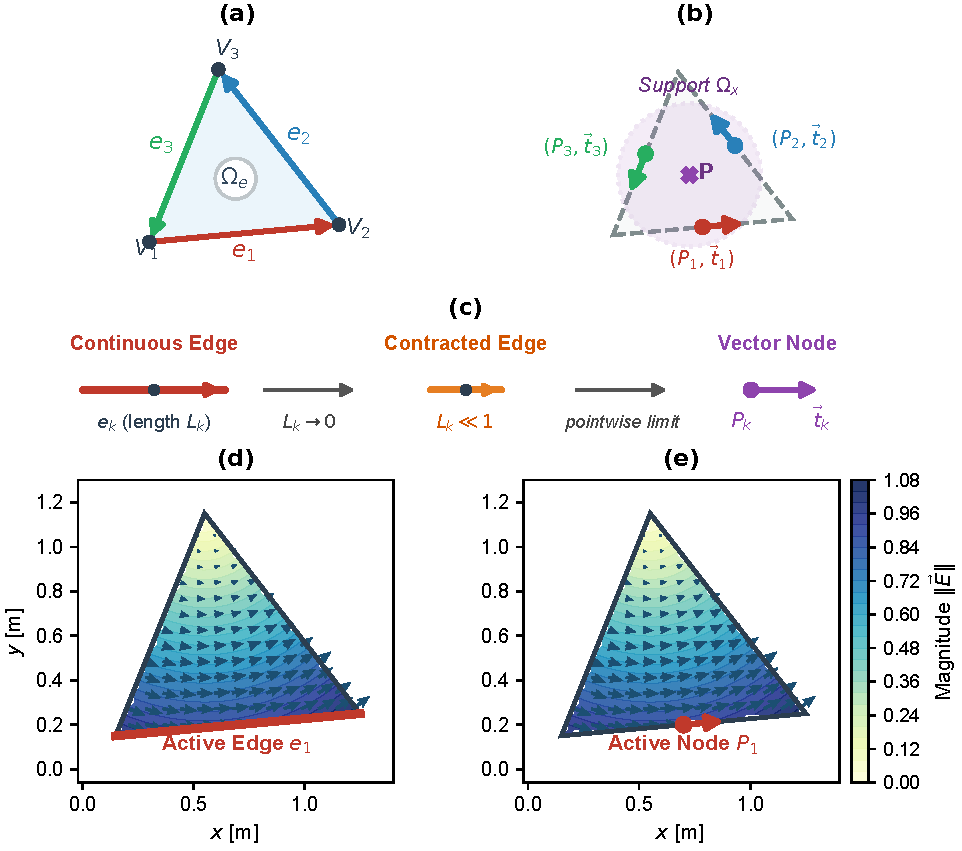
\includegraphics[width=\textwidth]{figura_equivalencia_dual_whitney_vnmm.pdf}
    \caption{Local equivalence between Whitney edge elements and the VNMM $\mathcal{L}^1$ basis.
        (a) Triangular cell $\Omega_e$ with vertices $V_i$ and oriented edges $e_k$;
        (b) VNMM support stencil with vector nodes $(P_k, \vec{t}_k)$ placed at edge midpoints;
        (c) Asymptotic collapse ($L_k \to 0$) mapping edge circulations to directional projections $e_k$;
        (d) Whitney 1-form $\vec{w}_1$ for edge $e_1$;
        (e) Normalized VNMM basis $\vec{N}_1/L_1$ for node $(P_1, \vec{t}_1)$, displaying identical vector fields over $\Omega_e$.}
    \label{fig:whitney_vnmm_dual_equivalence}
\end{figure*}


In conventional FEM (Fig.~\ref{fig:whitney_vnmm_dual_equivalence}a), the degrees of freedom associated with the triangular cell $\Omega_e$ are line integrals of circulation $\alpha_k = \oint_{e_k} \vec{E} \cdot d\boldsymbol{\ell}$ along continuous 1D edges of finite physical length $L_k$. As demonstrated in the asymptotic collapse limit (Fig.~\ref{fig:whitney_vnmm_dual_equivalence}c), when the physical edge length shrinks to zero ($L_k \to 0$), the 1D continuous edge degenerates into a point-collocated vector node $(P_k, \vec{t}_k)$, where the circulation DoF $\alpha_k$ naturally scales into a pointwise directional field projection $e_k = \vec{E}(P_k) \cdot \vec{t}_k$ [Volts/meter].

\subsubsection{Formal Proof of the Local Dual Equivalence Theorem}
\label{subsubsec:formal_proof_dual_whitney}
Let $T \subset \mathbb{R}^2$ be an arbitrary non-degenerate triangular simplex with vertices $V_1, V_2, V_3$ ordered counter-clockwise and non-zero area $|T| > 0$. Let $e_k = (V_k, V_{k+1})$ be the directed boundary edges of length $L_k = \|V_{k+1} - V_k\| > 0$, with unit tangent vectors $\vec{t}_k = (V_{k+1} - V_k)/L_k$ and midpoints $M_k = \frac{1}{2}(V_k + V_{k+1})$ for $k \in \{1, 2, 3\}$ (with index wrap-around $V_4 \equiv V_1$).

\begin{theorem}[Local Constructive Equivalence under Conforming Midpoint/Tangent Placement]
    \label{thm:dual_equivalence}
    Consider the support triad of vector nodes $\{P_k, \vec{t}_k\}_{k=1}^3$ defined at the edge midpoints $P_k = M_k$ with directors $\vec{t}_k$. The VNMM 2D $\mathcal{L}^1$ shape functions $\vec{N}_k(\mathbf{x})$ and the Whitney 1-forms $\vec{w}_k(\mathbf{x}) = \lambda_i(\mathbf{x})\nabla\lambda_j - \lambda_j(\mathbf{x})\nabla\lambda_i$ (with $(i,j)=(k,k+1)$) satisfy:
    \begin{equation}
        \vec{N}_k(\mathbf{x}) \equiv L_k \, \vec{w}_k(\mathbf{x}) \quad \Longleftrightarrow \quad \vec{w}_k(\mathbf{x}) \equiv \frac{1}{L_k} \vec{N}_k(\mathbf{x}), \quad \forall \mathbf{x} \in \mathbb{R}^2, \ \forall k \in \{1, 2, 3\}
        \label{eq:dual_equivalence_scaling}
    \end{equation}
\end{theorem}

\begin{proof}
    The proof proceeds in five constructive steps:

    \textbf{Step 1: Identity of Local Vector Polynomial Spaces.}
    The lowest-order Whitney space $\mathcal{W}(T)$ on $T$ is spanned by $\vec{w}_k(\mathbf{x}) = [a_1 + \alpha y, a_2 - \alpha x]^T$. By inspection of the spanning vectors, $\mathcal{W}(T) = \operatorname{span}\{[1,0]^T$, $[0,1]^T$, $[y,-x]^T\} \equiv \mathcal{L}^1$. Thus, both approximation spaces share identical 3-dimensional vector polynomial spaces.

    \textbf{Step 2: Constancy of Tangential Field Projection Along Simplex Edges.}
    Let $\vec{u}(\mathbf{x}) = [a_1 + \alpha y, a_2 - \alpha x]^T \in \mathcal{L}^1$. The directional projection of $\vec{u}(\mathbf{x})$ along unit director $\vec{t}_k = [\Delta x_k / L_k, \Delta y_k / L_k]^T$ is:
    \begin{equation}
        \vec{u}(\mathbf{x}) \cdot \vec{t}_k = \frac{1}{L_k} \left[ a_1 \Delta x_k + a_2 \Delta y_k + \alpha (y \Delta x_k - x \Delta y_k) \right]
    \end{equation}
    Since any point $\mathbf{x} = (x,y)$ on edge $e_k$ satisfies $(x - x_k)\Delta y_k - (y - y_k)\Delta x_k = 0$, the rotational term $y \Delta x_k - x \Delta y_k = y_k \Delta x_k - x_k \Delta y_k$ is strictly constant along the entire edge length. Therefore, the tangential projection is invariant along $e_k$:
    \begin{equation}
        \vec{u}(\mathbf{x}) \cdot \vec{t}_k = \vec{u}(M_k) \cdot \vec{t}_k, \quad \forall \mathbf{x} \in e_k
        \label{eq:edge_constancy}
    \end{equation}

    \textbf{Step 3: Reduction of Edge Circulation to Pointwise Midpoint Value.}
    Using Eq.~\eqref{eq:edge_constancy}, the line integral defining the FEM circulation degree of freedom along edge $e_j$ simplifies to:
    \begin{equation}
        \oint_{e_j} \vec{u} \cdot d\boldsymbol{\ell} = \int_{-L_j/2}^{L_j/2} \left( \vec{u}(\mathbf{x}(s)) \cdot \vec{t}_j \right) ds = \left( \vec{u}(M_j) \cdot \vec{t}_j \right) \int_{-L_j/2}^{L_j/2} ds = L_j \left( \vec{u}(M_j) \cdot \vec{t}_j \right)
    \end{equation}
    Substituting the $k$-th Whitney basis function $\vec{w}_k \in \mathcal{W}(T)$, which satisfies $\oint_{e_j} \vec{w}_k \cdot d\boldsymbol{\ell} = \delta_{jk}$ by construction, yields:
    \begin{equation}
        L_j \left( \vec{w}_k(M_j) \cdot \vec{t}_j \right) = \delta_{jk} \quad \implies \quad \left( L_k \vec{w}_k(M_j) \right) \cdot \vec{t}_j = \delta_{jk}
        \label{eq:whitney_midpoint_proj}
    \end{equation}

    \textbf{Step 4: Uniqueness and Exact Identification with VNMM Shape Functions.}
    By definition of the VNMM 2D $\mathcal{L}^1$ interpolation problem on the support triad $\{M_j, \vec{t}_j\}_{j=1}^3$, the shape functions satisfy $\vec{N}_k(M_j) \cdot \vec{t}_j = \delta_{jk}$. Consider the difference field:
    \begin{equation}
        \vec{d}_k(\mathbf{x}) = \vec{N}_k(\mathbf{x}) - L_k \vec{w}_k(\mathbf{x}) \in \mathcal{L}^1
    \end{equation}
    Evaluating its projection at each midpoint $M_j$:
    \begin{equation}
        \vec{d}_k(M_j) \cdot \vec{t}_j = \vec{N}_k(M_j) \cdot \vec{t}_j - L_k \left( \vec{w}_k(M_j) \cdot \vec{t}_j \right) = \delta_{jk} - \delta_{jk} = 0, \quad \forall j \in \{1, 2, 3\}
    \end{equation}
    By Steps 2--3, $\vec{d}_k$ has zero circulation along every edge, and edge circulations are unisolvent on $\mathcal{W}(T)=\mathcal{L}^1$ for non-degenerate $T$; hence $\vec{d}_k \equiv \mathbf{0}$ (equivalently, the local moment placement matrix $\mathbf{A} \in \mathbb{R}^{3 \times 3}$ is non-singular with $\det \mathbf{A} \neq 0$), which proves the exact identity $\vec{N}_k(\mathbf{x}) \equiv L_k \vec{w}_k(\mathbf{x})$ everywhere in $\mathbb{R}^2$.

    \textbf{Step 5: Verification of Differential Invariants.}
    1. \textit{Divergence:} For any field $\vec{u} = [a_1 + \alpha y, a_2 - \alpha x]^T \in \mathcal{L}^1$, we have $\nabla \cdot \vec{u} = \partial(a_1 + \alpha y)/\partial x + \partial(a_2 - \alpha x)/\partial y \equiv 0$. Thus, $\nabla \cdot \vec{w}_k \equiv 0$ and $\nabla \cdot \vec{N}_k \equiv 0$ everywhere.
    2. \textit{Curl:} Applying Stokes' theorem over triangle $T$ for Whitney 1-form $\vec{w}_k$:
    \begin{equation}
        \int_T (\nabla \times \vec{w}_k)_z d\Omega = \oint_{\partial T} \vec{w}_k \cdot d\boldsymbol{\ell} = \sum_{j=1}^3 \delta_{jk} = 1 \implies (\nabla \times \vec{w}_k)_z = \frac{1}{|T|}
    \end{equation}
    By the identity proved in step 4, $(\nabla \times \vec{N}_k)_z = L_k (\nabla \times \vec{w}_k)_z = L_k / |T|$.
\end{proof}

As graphically illustrated in Fig.~\ref{fig:whitney_vnmm_dual_equivalence}d and~\ref{fig:whitney_vnmm_dual_equivalence}e (and verified numerically in Section~\ref{subsec:conforming_dual_equivalence}), the normalized VNMM $\mathcal{L}^1$ shape functions $\frac{1}{L_k}\vec{N}_k$ and canonical Whitney 1-forms $\vec{w}_k$ match identically across the simplex $T$ down to floating-point machine precision ($\approx 10^{-16}$).

\subsubsection{Local \texorpdfstring{$H(\mathbf{curl})$}{H(curl)} Regularity versus Global \texorpdfstring{$H(\mathbf{curl})$}{H(curl)} Conformity}
Beyond establishing the mathematical connection to edge finite elements, this constructive identity clarifies a fundamental structural distinction in vector meshless approximations:
\begin{enumerate}
    \item \textbf{Local $H(\mathbf{curl})$ Regularity on Virtual Simplices:} In conventional scalar meshless methods (e.g., Moving Least Squares or Element-Free Galerkin), evaluating field approximations outside the physical convex hull enclosed by the node coordinates $\mathbf{x}_k$ constitutes an unconstrained extrapolation, leading to rapid truncation error growth \cite{lima2017edge}. In contrast, because the VNMM vector basis reproduces the complete polynomial space of Whitney edge elements over the virtual macro-triangle $\Omega_{x}$ defined by the intersecting lines of action of vector directors $\vec{t}_k$ (Fig.~\ref{fig:whitney_vnmm_dual_equivalence}b), the valid domain for local $H(\mathbf{curl})$ field approximation is not geographically restricted to the small physical convex hull of $\mathbf{x}_k$ \cite{nedelec1980mixed, monk2003finite}. Under regular-support assumptions (well-conditioned local placement matrix $\mathbf{A}$ and non-degenerate intersection vertices), any field evaluation at $P \in \Omega_{x}$ preserves local $H(\mathbf{curl})$ regularity.
    \item \textbf{Loss of Global $H(\mathbf{curl})$ Conformity on Unconstrained Point Clouds:} When nodes and directors form a conforming simplicial mesh (Section~\ref{subsubsec:formal_proof_dual_whitney}), tangential traces across adjacent element facets match identically, yielding global conformity $V_h \subset H(\mathbf{curl}; \Omega)$. On arbitrary, unconstrained point clouds, however, support stencils are selected dynamically as the evaluation point $P$ moves across the domain. Because adjacent stencils differ in node composition and orientation, tangential traces do not cancel continuously across internal support boundaries. Consequently, the global approximation space is non-conforming ($V_h \not\subset H(\mathbf{curl}; \Omega)$). As developed later in Section~\ref{sec:variational_formulation}, this distinction is essential: while local polynomial completeness (via $\mathcal{P}^1$, Section~\ref{subsec:complete_P1_basis}) restores local Jacobian and curl consistency, global non-conformity impacts the discrete de Rham complex and requires variational stabilization in boundary-value and eigenvalue problems.
\end{enumerate}

\subsubsection{Mathematical Origin of Modal Aliasing and Curl Stagnation}
\label{subsec:L1_aliasing_analysis}

While the incomplete solenoidal basis $\mathcal{L}^1$ exhibits exact dual equivalence to Whitney elements on conforming meshes (Section~\ref{subsubsec:dual_whitney}), its behavior diverges sharply on unconstrained point clouds, where curl approximations stagnate at an $\mathcal{O}(1)$ relative error plateau under spatial refinement (as numerically confirmed in Section~\ref{subsubsec:curl_stagnation_L1} and Fig.~\ref{fig:convergencia_interpolacao_L1_vs_P1}b). To uncover the algebraic origin of this derivative stagnation, we examine the local Taylor series expansion of the exact electric field $\vec{E}$ centered at an evaluation point $P(x_P, y_P)$ \cite{li2007meshfree, liu2009mesh}:
\begin{equation}
    \vec{E}(\mathbf{x}) = \vec{E}(P) + \mathbf{J}(P) \begin{bmatrix} \Delta x \\[2pt] \Delta y \end{bmatrix} + \mathcal{O}(h^2)
    \label{eq:taylor_vector_expansion}
\end{equation}
where $\mathbf{J}(P) = \nabla \vec{E}$ represents the complete first-order field Jacobian tensor \cite{liu2009mesh}:
\begin{equation}
    \mathbf{J} = \begin{bmatrix}
        \frac{\partial E_x}{\partial x} & \frac{\partial E_x}{\partial y} \\[4pt]
        \frac{\partial E_y}{\partial x} & \frac{\partial E_y}{\partial y}
    \end{bmatrix}
    \label{eq:jacobian_tensor_raw}
\end{equation}

By expressing individual spatial derivatives in terms of fundamental vector calculus operators---namely, the field divergence $\nabla \cdot \vec{E} = \partial E_x/\partial x + \partial E_y/\partial y$ and the z-directed field curl $(\nabla \times \vec{E})_z = \partial E_y/\partial x - \partial E_x/\partial y$---the field Jacobian tensor is decomposed as:
\begin{equation}
    \mathbf{J} = \frac{1}{2}(\nabla \cdot \vec{E}) \mathbf{I} + \frac{1}{2}(\nabla \times \vec{E})_z \begin{bmatrix} 0 & -1 \\ 1 & 0 \end{bmatrix} + \begin{bmatrix} \delta_{\mathrm{norm}} & \delta_{\mathrm{trans}} \\ \delta_{\mathrm{trans}} & -\delta_{\mathrm{norm}} \end{bmatrix}
    \label{eq:jacobian_tensor_EM_decomposition}
\end{equation}
where $\delta_{\mathrm{norm}} = \frac{1}{2}(\partial E_x/\partial x - \partial E_y/\partial y)$ denotes the normal (longitudinal) field derivative difference, and $\delta_{\mathrm{trans}} = \frac{1}{2}(\partial E_y/\partial x + \partial E_x/\partial y)$ represents the symmetric transverse (shear) field derivative component.

In the incomplete $\mathcal{L}^1$ basis, local shape functions provide only 3 degrees of freedom. As a result, normal field derivatives are artificially forced to vanish identically ($\partial E_x^h/\partial x \equiv 0$ and $\partial E_y^h/\partial y \equiv 0$), imposing $\nabla \cdot \vec{E}^h \equiv 0$, $\delta_{\mathrm{norm}} \equiv 0$, and $\delta_{\mathrm{trans}} \equiv 0$ simultaneously.

This fundamental limitation is formalized in the following proposition:

\begin{proposition}[Jacobian Incompleteness and Derivative Modal Aliasing Scaling]
    \label{prop:L1_aliasing}
    Let $\vec{E} \in [C^2(\Omega)]^2$ be an arbitrary twice continuously differentiable 2D vector field. The incomplete solenoidal space $\mathcal{L}^1 = \operatorname{span}\{[1, 0]^T, [0, 1]^T, [y, -x]^T\} \subset \mathcal{P}_1 \times \mathcal{P}_1$ cannot reproduce the complete first-order Taylor expansion of $\vec{E}$. Specifically, while the complete space $\mathcal{P}^1 = \mathcal{P}_1 \times \mathcal{P}_1$ possesses $\dim(\mathcal{P}^1) = 6$ degrees of freedom to reconstruct the 2 translation components and all 4 independent entries of the Jacobian tensor $\mathbf{J} = \nabla\vec{E}$, $\mathcal{L}^1$ possesses only $\dim(\mathcal{L}^1) = 3$ degrees of freedom, enforcing the artificial linear constraints:
    \begin{equation}
        \frac{\partial E_x^h}{\partial x} = 0, \quad \frac{\partial E_y^h}{\partial y} = 0, \quad \text{and} \quad \frac{\partial E_x^h}{\partial y} + \frac{\partial E_y^h}{\partial x} = 0.
        \label{eq:L1_derivative_constraints}
    \end{equation}
    Under point-collocated projection on unstructured node clouds, unrepresented normal gradients ($\partial E_x/\partial x, \partial E_y/\partial y \neq 0$) generate a local projection remainder $\mathbf{r} \sim \mathcal{O}(h)$ that couples into the rotational coefficient through the inverted moment placement matrix row $\operatorname{Row}_3(\mathbf{A}^{-1}) \sim \mathcal{O}(h^{-1})$. In an asymptotic order-of-magnitude scaling sense, this generically induces an $\mathcal{O}(1)$ derivative aliasing error in the pointwise reconstructed curl under refinement ($h \to 0$) in the collocated setting:
    \begin{equation}
        |(\nabla \times \vec{E})_z - (\nabla \times \vec{E}^h)_z| \sim \|\operatorname{Row}_3(\mathbf{A}^{-1})\| \|\mathbf{r}\| = \mathcal{O}(h^{-1}) \cdot \mathcal{O}(h) = \mathcal{O}(1).
        \label{eq:aliasing_order_proof}
    \end{equation}
\end{proposition}

\begin{proof}
    Let any discrete vector field $\vec{E}^h \in \mathcal{L}^1$ be expanded in terms of the solenoidal basis:
    \begin{equation}
        \vec{E}^h(x, y) = a \begin{bmatrix} 1 \\ 0 \end{bmatrix} + b \begin{bmatrix} 0 \\ 1 \end{bmatrix} + c \begin{bmatrix} y \\ -x \end{bmatrix}, \quad a, b, c \in \mathbb{R}.
        \label{eq:proof_L1_expansion}
    \end{equation}
    Direct differentiation with respect to spatial coordinates yields the discrete Jacobian tensor:
    \begin{equation}
        \mathbf{J}^h = \begin{bmatrix}
            \frac{\partial E_x^h}{\partial x} & \frac{\partial E_x^h}{\partial y} \\[4pt]
            \frac{\partial E_y^h}{\partial x} & \frac{\partial E_y^h}{\partial y}
        \end{bmatrix} = \begin{bmatrix}
            0  & c \\
            -c & 0
        \end{bmatrix}.
        \label{eq:proof_discrete_jacobian}
    \end{equation}
    Inspect Eq.~\eqref{eq:proof_discrete_jacobian} establishes that $\partial E_x^h/\partial x \equiv 0$, $\partial E_y^h/\partial y \equiv 0$, and $\partial E_x^h/\partial y + \partial E_y^h/\partial x = c - c \equiv 0$, identically satisfying the linear constraints in Eq.~\eqref{eq:L1_derivative_constraints}.

    Now consider a general smooth physical field $\vec{E} \in [C^2(\Omega)]^2$. Its Taylor expansion centered at evaluation point $P$ is $\vec{E}(\mathbf{x}) = \vec{E}(P) + \mathbf{J}(P) \Delta\mathbf{x} + \mathcal{O}(h^2)$, where $\mathbf{J}(P)$ has non-zero diagonal entries ($\partial E_x/\partial x \neq 0$ or $\partial E_y/\partial y \neq 0$). Collocating $\vec{E}^h$ at support nodes $\mathbf{x}_k$ ($k=1,2,3$) along unit directors $\vec{t}_k$ defines the linear placement system $\mathbf{A} [a, b, c]^T = \mathbf{e}$, where $e_k = \vec{E}(\mathbf{x}_k) \cdot \vec{t}_k$.

    Subtracting the projection of the unrepresented linear components $(\mathbf{J}(P) - \mathbf{J}^h) \Delta\mathbf{x}_k \cdot \vec{t}_k$ yields a nodal projection residual $\mathbf{r} \in \mathbb{R}^3$ with asymptotic magnitude $\|\mathbf{r}\| \sim \mathcal{O}(h)$. In the $3 \times 3$ moment placement matrix $\mathbf{A}$ (Eq.~\eqref{eq:matrix_A_L1}), translation columns 1--2 scale as $\mathcal{O}(1)$, while the rotational moment column 3 scales as $(\Delta y_k t_{kx} - \Delta x_k t_{ky}) \sim \mathcal{O}(h)$. Consequently, by Cramer's rule or Neumann inversion, the third row of $\mathbf{A}^{-1}$ (which maps nodal data to the rotational DoF $c = -\frac{1}{2}(\nabla \times \vec{E}^h)_z$) scales strictly as $\|\operatorname{Row}_3(\mathbf{A}^{-1})\| \sim \mathcal{O}(h^{-1})$.

    The numerical error in the reconstructed curl at evaluation point $P$ is therefore governed by the propagation of the projection remainder:
    \begin{equation}
        \begin{aligned}
            |(\nabla \times \vec{E})_z - (\nabla \times \vec{E}^h)_z| & = 2 |c_{\mathrm{exact}} - c|                                                                                               \\
                                                                      & \sim \|\operatorname{Row}_3(\mathbf{A}^{-1})\| \|\mathbf{r}\| = \mathcal{O}(h^{-1}) \cdot \mathcal{O}(h) = \mathcal{O}(1),
        \end{aligned}
    \end{equation}
    which is asymptotically independent of $h$ and generates an $\mathcal{O}(1)$ error plateau under spatial refinement ($h \to 0$) in the collocated setting for generic node/director placements (see Remark~\ref{rem:prop1_scope}).
\end{proof}

\begin{remark}[Scope of Proposition~\ref{prop:L1_aliasing} and the Conforming Case]
    \label{rem:prop1_scope}
    The estimate is an order-of-magnitude bound, attained only when the weights of $\operatorname{Row}_3(\mathbf{A}^{-1})$ fail to annihilate the unrepresented symmetric part $\mathbf{S}$ of $\mathbf{J}$. In the conforming midpoint/tangent configuration of Theorem~\ref{thm:dual_equivalence}, $\operatorname{Row}_3(\mathbf{A}^{-1})_k \propto L_k/|T|$ and the residual satisfies $\sum_k L_k r_k = \oint_{\partial T}(\mathbf{S}\mathbf{x})\cdot d\boldsymbol{\ell} = \int_T \nabla\times(\mathbf{S}\mathbf{x})\,d\Omega = 0$, since $\sum_k L_k \vec{t}_k=\mathbf{0}$, the midpoint rule is exact for linear integrands, and $\nabla\times(\mathbf{S}\mathbf{x})=0$ for symmetric $\mathbf{S}$. The residual therefore does not reach the curl degree of freedom, consistently with the $\mathcal{O}(h)$ curl error of Whitney elements. The $\mathcal{O}(1)$ plateau should thus be read as the generic behaviour on arbitrary node/director placements, where this closed-contour cancellation is not satisfied; it is confirmed numerically (Section~\ref{subsec:arbitrary_meshless_interpolation}) rather than proved for all clouds.
\end{remark}

In Edge Finite Element Methods (EFEM), this lack of explicit normal derivative representation does not cause stagnation because continuous line circulation integrals along element edges enforce closed-contour flux cancellation via Stokes' theorem \cite{nedelec1980mixed, monk2003finite}. On arbitrary clouds, however, the weights of $\operatorname{Row}_3(\mathbf{A}^{-1})$ are no longer the closed-contour circulation weights $L_k/|T|$ of Whitney elements, so this cancellation is not guaranteed. Consequently, the $\mathcal{O}(1)$ derivative noise floor established in Proposition~\ref{prop:L1_aliasing} cannot be eliminated by spatial mesh refinement alone ($h \to 0$). Adopting the complete linear polynomial vector space $\mathcal{P}^1 = \mathcal{P}_1 \times \mathcal{P}_1$, as formulated in Section~\ref{subsec:complete_P1_basis}, provides a direct and sufficient remedy by resolving the complete local Jacobian and eliminating this specific derivative-aliasing mechanism on unconstrained point clouds.


% ---------------------------------------------------------
% SUBSECTION 2.3: THE COMPLETE P1 VECTOR POLYNOMIAL BASIS
% ---------------------------------------------------------
\subsection{The Complete \texorpdfstring{$\mathcal{P}^1$}{P1} Vector Polynomial Basis}
\label{subsec:complete_P1_basis}

To eliminate the derivative modal aliasing and curl stagnation inherent to the incomplete $\mathcal{L}^1$ space, we reformulate local vector interpolation using the complete linear polynomial vector space $\mathcal{P}^1 = \mathcal{P}_1 \times \mathcal{P}_1$. This transition draws a direct mathematical analogy to Nédélec's second family of mixed finite elements \cite{nedelec1986new}, in which vector field approximations are constructed over complete polynomial spaces $(\mathbb{P}_k)^d$ rather than solenoidal-restricted subspaces.

In two dimensions ($d=2$), a complete first-order vector polynomial basis $\mathcal{P}^1$ provides 6 independent degrees of freedom ($M_{\mathrm{supp}} = 6$ support nodes per evaluation point):
\begin{equation}
    \mathcal{P}^1 = \operatorname{span} \left\{
    \begin{bmatrix} 1 \\ 0 \end{bmatrix},
    \begin{bmatrix} 0 \\ 1 \end{bmatrix},
    \begin{bmatrix} x \\ 0 \end{bmatrix},
    \begin{bmatrix} y \\ 0 \end{bmatrix},
    \begin{bmatrix} 0 \\ x \end{bmatrix},
    \begin{bmatrix} 0 \\ y \end{bmatrix}
    \right\}
    \label{eq:complete_P1_basis_vectors}
\end{equation}

Using this complete basis, the local vector shape function $\vec{N}_i(\mathbf{x})$ associated with the $i$-th support node is expressed as a linear combination of its six constituent terms:
\begin{equation}
    \vec{N}_i(x, y) = \beta_{1i} \begin{bmatrix} 1 \\ 0 \end{bmatrix} + \beta_{2i} \begin{bmatrix} 0 \\ 1 \end{bmatrix} + \beta_{3i} \begin{bmatrix} x \\ 0 \end{bmatrix} + \beta_{4i} \begin{bmatrix} y \\ 0 \end{bmatrix} + \beta_{5i} \begin{bmatrix} 0 \\ x \end{bmatrix} + \beta_{6i} \begin{bmatrix} 0 \\ y \end{bmatrix}
    \label{eq:P1_shape_function_expansion}
\end{equation}
where $\beta_{ji}$ (for $j=1, \dots, 6$) represent the local interpolation coefficients to be determined.

Enforcing the vector Kronecker delta projection property \cite{ortiz2021nodal}:
\begin{equation}
    \vec{N}_i(\mathbf{x}_k) \cdot \vec{t}_k = \delta_{ik}, \quad \text{for } k = 1, \dots, 6
    \label{eq:kronecker_projection_P1}
\end{equation}
across all six support nodes yields the local linear placement system
\begin{equation}
    \mathbf{A} \boldsymbol{\beta}_i = \mathbf{L}_i.
    \label{eq:linear_system_P1}
\end{equation}
Evaluated in local translated coordinates centered at the evaluation point $P(x_P, y_P)$ (defined as $\Delta x_k = x_k - x_P$ and $\Delta y_k = y_k - y_P$), the local moment placement matrix $\mathbf{A} \in \mathbb{R}^{6 \times 6}$ is explicitly given by:
\begin{equation}
    \mathbf{A} = \begin{bmatrix}
        t_{1x} & t_{1y} & \Delta x_1 t_{1x} & \Delta y_1 t_{1x} & \Delta x_1 t_{1y} & \Delta y_1 t_{1y} \\[4pt]
        t_{2x} & t_{2y} & \Delta x_2 t_{2x} & \Delta y_2 t_{2x} & \Delta x_2 t_{2y} & \Delta y_2 t_{2y} \\[4pt]
        t_{3x} & t_{3y} & \Delta x_3 t_{3x} & \Delta y_3 t_{3x} & \Delta x_3 t_{3y} & \Delta y_3 t_{3y} \\[4pt]
        t_{4x} & t_{4y} & \Delta x_4 t_{4x} & \Delta y_4 t_{4x} & \Delta x_4 t_{4y} & \Delta y_4 t_{4y} \\[4pt]
        t_{5x} & t_{5y} & \Delta x_5 t_{5x} & \Delta y_5 t_{5x} & \Delta x_5 t_{5y} & \Delta y_5 t_{5y} \\[4pt]
        t_{6x} & t_{6y} & \Delta x_6 t_{6x} & \Delta y_6 t_{6x} & \Delta x_6 t_{6y} & \Delta y_6 t_{6y}
    \end{bmatrix}
    \label{eq:matrix_A_6x6}
\end{equation}

The corresponding coefficient vector $\boldsymbol{\beta}_i$ and canonical right-hand side vector $\mathbf{L}_i$ are structured as:
\begin{equation}
    \boldsymbol{\beta}_i = \begin{bmatrix} \beta_{1i} \\[2pt] \beta_{2i} \\[2pt] \beta_{3i} \\[2pt] \beta_{4i} \\[2pt] \beta_{5i} \\[2pt] \beta_{6i} \end{bmatrix}, \qquad
    \mathbf{L}_i = \begin{bmatrix} \delta_{1i} \\[2pt] \delta_{2i} \\[2pt] \delta_{3i} \\[2pt] \delta_{4i} \\[2pt] \delta_{5i} \\[2pt] \delta_{6i} \end{bmatrix}
    \label{eq:beta_and_L_vectors_P1}
\end{equation}

Solving the linear system~\eqref{eq:linear_system_P1} via $\boldsymbol{\beta}_i = \mathbf{A}^{-1} \mathbf{L}_i$ completely defines the vector shape functions $\vec{N}_i(\mathbf{x})$. Consequently, the approximated electric field $\vec{E}^h(\mathbf{x})$ and its z-directed curl $(\nabla \times \vec{E}^h)_z$ within the support domain are expressed analytically as:
\begin{align}
    \vec{E}^h(x, y)                   & = \sum_{i=1}^6 \vec{N}_i(x, y) e_i \label{eq:field_approximation_P1}                                                                                  \\[4pt]
    (\nabla \times \vec{E}^h)_z(x, y) & = \frac{\partial E_y^h}{\partial x} - \frac{\partial E_x^h}{\partial y} = \sum_{i=1}^6 (\beta_{5i} - \beta_{4i}) e_i \label{eq:curl_approximation_P1}
\end{align}
where $e_i = \vec{E}(P_i) \cdot \vec{t}_i$ denotes the scalar directional projection degree of freedom associated with the $i$-th node.

By providing 6 independent degrees of freedom, the complete $\mathcal{P}^1$ space resolves all four spatial derivative components of the local Jacobian tensor $\mathbf{J}^h = \nabla \vec{E}^h$ simultaneously:
\begin{equation}
    \mathbf{J}^h = \begin{bmatrix}
        \frac{\partial E_x^h}{\partial x} & \frac{\partial E_x^h}{\partial y} \\[4pt]
        \frac{\partial E_y^h}{\partial x} & \frac{\partial E_y^h}{\partial y}
    \end{bmatrix} = \sum_{i=1}^6 \begin{bmatrix}
        \beta_{3i} & \beta_{4i} \\[4pt]
        \beta_{5i} & \beta_{6i}
    \end{bmatrix} e_i
    \label{eq:full_jacobian_tensor_P1}
\end{equation}

Unlike the incomplete $\mathcal{L}^1$ space, which artificially forces longitudinal (normal) field derivatives ($\partial E_x/\partial x$, $\partial E_y/\partial y$) to vanish, the complete $\mathcal{P}^1$ basis resolves both rotational and irrotational (longitudinal flux variation) components simultaneously. This shields the field curl calculation from longitudinal derivative truncation residues, removing the derivative modal aliasing mechanism and providing the polynomial consistency required for first-order curl convergence, while yielding an observed convergence rate of $\mathcal{O}(h^{2.17})$ for electric field interpolation in the investigated benchmark (Section~\ref{subsec:arbitrary_meshless_interpolation}).

% =========================================================
% SECTION 3: ALGEBRAIC CONDITIONING AND SUPPORT SELECTION
% =========================================================
\section{Algebraic Conditioning and Support Selection}
\label{sec:conditioning}

The construction of vector nodal shape functions $\vec{N}_i$ in the Vector Nodal Meshless Method (VNMM) relies on solving the local linear placement system $\mathbf{A} \boldsymbol{\beta}_i = \mathbf{L}_i$ (Eq.~\eqref{eq:linear_system_P1}). A fundamental prerequisite for the existence, uniqueness, and numerical stability of these vector shape functions is that the local moment placement matrix $\mathbf{A}$ remains strictly non-singular ($|\det(\mathbf{A})| > 0$).

Unlike scalar meshless formulations where matrix singularity is dictated purely by spatial nodal distributions (e.g., node co-location or spatial co-linearity), the conditioning of $\mathbf{A}$ in the VNMM is intrinsically coupled to both the spatial coordinates $\mathbf{x}_k = (x_k, y_k)$ and the orientation of the unit vector directors $\vec{t}_k = [t_{kx}, t_{ky}]^T$ assigned to each support node. In the following subsections, a detailed algebraic singularity analysis is conducted for both the incomplete $\mathcal{L}^1$ basis (Section~\ref{subsec:singularities_L1}) and the complete $\mathcal{P}^1$ basis (Section~\ref{subsec:singularities_P1}), establishing the mathematical foundation for the automated support selection strategy developed in Section~\ref{subsec:scale_invariant_criterion}.


% ---------------------------------------------------------
% SUBSECTION 3.1: L1 BASIS SINGULARITIES (3x3 MATRIX)
% ---------------------------------------------------------
\subsection{Singularities and Geometric Constraints in the Incomplete \texorpdfstring{$\mathcal{L}^1$}{L1} Basis (\texorpdfstring{$3 \times 3$}{3x3} Matrix)}
\label{subsec:singularities_L1}

To establish a systematic classification of algebraic singularities in the original VNMM 2D formulation \cite{ortiz2021nodal, ortiz2023tese}, we revisit the $3 \times 3$ local moment placement matrix $\mathbf{A}$ generated by the 3-node solenoidal basis $\mathcal{L}^1$. Originally derived in Eq.~\eqref{eq:matrix_A_L1}, $\mathbf{A}$ is restated below to facilitate the singularity analysis:
\begin{equation}
    \mathbf{A} = \begin{bmatrix}
        t_{1x} & t_{1y} & y_1 t_{1x} - x_1 t_{1y} \\[4pt]
        t_{2x} & t_{2y} & y_2 t_{2x} - x_2 t_{2y} \\[4pt]
        t_{3x} & t_{3y} & y_3 t_{3x} - x_3 t_{3y}
    \end{bmatrix}
    \label{eq:matrix_A_L1_revisited}
\end{equation}

For this matrix, algebraic singularity ($\det(\mathbf{A}) = 0$) occurs when the spatial-directional equations contributed by the candidate triad become linearly dependent. As classified visually in Figs.~\ref{fig:vnmm_singularities_matrix_A}a--\ref{fig:vnmm_singularities_matrix_A}d, these mathematical failures fall into four distinct pathological configurations:

\begin{figure*}[!t]
    \centering
    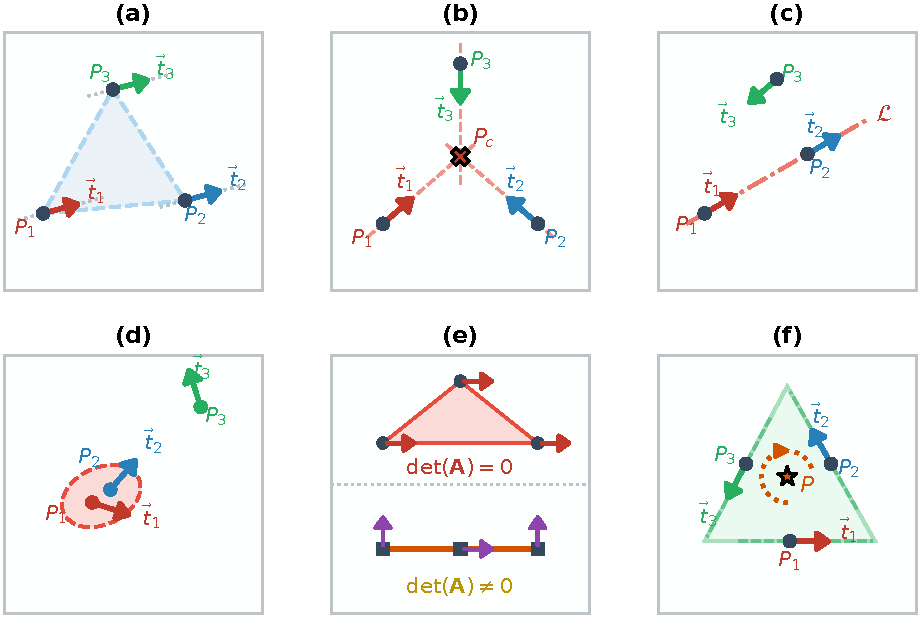
\includegraphics[width=\textwidth]{figura_singularidades_matriz_A.pdf}
    \caption{Singularity configurations and support qualification for the VNMM $\mathcal{L}^1$ placement matrix $\mathbf{A}$.
        (a) Global vector parallelism ($\vec{t}_1 \parallel \vec{t}_2 \parallel \vec{t}_3$);
        (b) Concurrent lines of action intersecting at focal point $P_c$;
        (c) Collinear nodes sharing a common line of action;
        (d) Nodal coincidence ($\|P_1 - P_2\| \to 0$);
        (e) Decoupling of nodal geometry and director alignment: spatially non-collinear nodes with parallel directors yield $\det(\mathbf{A}) = 0$ (top), whereas collinear nodes with non-parallel directors fail to span 2D derivatives (bottom);
        (f) Admissible support: non-collinear distribution ($\operatorname{Area}(T) > 0$) with non-vanishing circulation around evaluation point $P$.}
    \label{fig:vnmm_singularities_matrix_A}
\end{figure*}

\begin{enumerate}
    \item \textbf{Global Vector Parallelism (Fig.~\ref{fig:vnmm_singularities_matrix_A}a):} If all three unit directors are parallel or anti-parallel ($\vec{t}_1 \parallel \vec{t}_2 \parallel \vec{t}_3$), director components satisfy $t_{kx} = c \cdot t_{ky}$ for a constant scalar $c$. Thus, $\operatorname{Col}_1(\mathbf{A}) = c \cdot \operatorname{Col}_2(\mathbf{A})$, yielding $\det(\mathbf{A}) \equiv 0$ regardless of nodal spatial distribution.

    \item \textbf{Concurrency of Lines of Action (Fig.~\ref{fig:vnmm_singularities_matrix_A}b):} If the infinite lines of action passing through $\mathbf{x}_k$ along $\vec{t}_k$ intersect at a single common point $P_c(x_c, y_c)$, every node satisfies $t_{kx}(y_k - y_c) - t_{ky}(x_k - x_c) = 0$. This forces column $\operatorname{Col}_3$ to become a linear combination of the other two columns, $\operatorname{Col}_3 = y_c \operatorname{Col}_1 - x_c \operatorname{Col}_2$, causing $\det(\mathbf{A}) = 0$.

    \item \textbf{Overlapping Lines of Action (Fig.~\ref{fig:vnmm_singularities_matrix_A}c):} If two support nodes lie on a common line $\mathcal{L}$ with directors aligned parallel to $\mathcal{L}$, the second row becomes identical to the first ($\operatorname{Row}_2 = \operatorname{Row}_1$), causing rank deficiency ($\operatorname{rank}(\mathbf{A}) \le 2$).

    \item \textbf{Nodal Coincidence / Spatial Collapse (Fig.~\ref{fig:vnmm_singularities_matrix_A}d):} Shared spatial coordinates ($\mathbf{x}_i \approx \mathbf{x}_j$) collapse spatial moment sampling, preventing 2D vector interpolation span.
\end{enumerate}

\subsubsection{Decoupling of Spatial Geometry and Vector Alignment}
\label{subsubsec:decoupling_L1}

A crucial theoretical insight governing vector meshless approximations is the formal decoupling between spatial sampling quality and vector algebraic independence, as explicitly highlighted in Fig.~\ref{fig:vnmm_singularities_matrix_A}e:

\begin{itemize}
    \item \textbf{Spatially Ideal but Algebraically Singular (Fig.~\ref{fig:vnmm_singularities_matrix_A}e, top):} A candidate triad can form an optimal 2D spatial distribution (e.g., an equilateral triangle enclosing a large physical area $|T| > 0$). A purely spatial geometric filter or distance-based $k$-d tree query would readily accept this support. However, if the assigned vector directors are globally parallel ($\vec{t}_1 \parallel \vec{t}_2 \parallel \vec{t}_3$), matrix $\mathbf{A}$ is strictly singular ($\det(\mathbf{A}) = 0$), rendering shape function construction impossible.

    \item \textbf{Algebraically Solvable but Spatially Degenerate (Fig.~\ref{fig:vnmm_singularities_matrix_A}e, bottom):} Conversely, if three support nodes lie on a perfectly collinear 1D line in space (zero triangle area $|T| = 0$) but possess non-parallel directors, matrix $\mathbf{A}$ in the $\mathcal{L}^1$ basis can yield a non-zero determinant ($\det(\mathbf{A}) \neq 0$). While algebraically solvable, this configuration lacks 2D spatial sampling normal to the line of nodes, leading to unconstrained polynomial extrapolation and catastrophic derivative errors in field operators.

\end{itemize}
In contrast to the pathological or decoupled configurations depicted in Figs.~\ref{fig:vnmm_singularities_matrix_A}(a)--(e), an admissible support---designated as an ideal support triad in Fig.~\ref{fig:vnmm_singularities_matrix_A}(f)---requires a dual geometric-directional qualification. Geometrically, the candidate support nodes must form a non-degenerate 2D spatial distribution ($|T| > 0$), shielding the local domain from nodal collapse or spatial collinearity. Directionally, the assigned vector directors $\vec{t}_k$ must provide coherent tangential circulation around the evaluation point $P(x_P, y_P)$, maximizing the directional moment $M_k = (\Delta\mathbf{x}_k \times \vec{t}_k)_z \gg 0$.

% ---------------------------------------------------------
% SUBSECTION 3.2: SINGULARITY ANALYSIS IN THE COMPLETE P1 BASIS (6x6 MATRIX)
% ---------------------------------------------------------
\subsection{Singularity Analysis in the Complete \texorpdfstring{$\mathcal{P}^1$}{P1} Vector Basis (\texorpdfstring{$6 \times 6$}{6x6} Matrix)}
\label{subsec:singularities_P1}

Extending the singularity analysis to the complete vector basis $\mathcal{P}^1$ ($M_{\mathrm{supp}} = 6$), we consider the corresponding $6 \times 6$ local placement matrix $\mathbf{A} \in \mathbb{R}^{6 \times 6}$. Evaluated in local translated coordinates centered at the evaluation point $P(x_P, y_P)$ ($\Delta x_k = x_k - x_P, \Delta y_k = y_k - y_P$), matrix $\mathbf{A}$ (Eq.~\eqref{eq:matrix_A_6x6}) is restated below to facilitate the investigation:
\begin{equation}
    \mathbf{A} = \begin{bmatrix}
        t_{1x} & t_{1y} & \Delta x_1 t_{1x} & \Delta y_1 t_{1x} & \Delta x_1 t_{1y} & \Delta y_1 t_{1y} \\[4pt]
        t_{2x} & t_{2y} & \Delta x_2 t_{2x} & \Delta y_2 t_{2x} & \Delta x_2 t_{2y} & \Delta y_2 t_{2y} \\[4pt]
        t_{3x} & t_{3y} & \Delta x_3 t_{3x} & \Delta y_3 t_{3x} & \Delta x_3 t_{3y} & \Delta y_3 t_{3y} \\[4pt]
        t_{4x} & t_{4y} & \Delta x_4 t_{4x} & \Delta y_4 t_{4x} & \Delta x_4 t_{4y} & \Delta y_4 t_{4y} \\[4pt]
        t_{5x} & t_{5y} & \Delta x_5 t_{5x} & \Delta y_5 t_{5x} & \Delta x_5 t_{5y} & \Delta y_5 t_{5y} \\[4pt]
        t_{6x} & t_{6y} & \Delta x_6 t_{6x} & \Delta y_6 t_{6x} & \Delta x_6 t_{6y} & \Delta y_6 t_{6y}
    \end{bmatrix}
    \label{eq:matrix_A_P1_repeated}
\end{equation}

By the unisolvence principle for vector degrees of freedom \cite{monk2003finite} (here termed the Null-Space Orthogonality Principle), a non-zero coefficient vector $\mathbf{p} = [a_1, a_2, b_1, b_2, b_3, b_4]^T \in \mathbb{R}^6$ belongs to $\ker(\mathbf{A}_{6 \times 6})$ if and only if the corresponding affine vector field $\vec{E}(\mathbf{x}) \in \mathcal{P}^1$ (with components $E_x = a_1 + b_1 \Delta x + b_2 \Delta y$ and $E_y = a_2 + b_3 \Delta x + b_4 \Delta y$) satisfies the directional orthogonality condition $\vec{E}(\mathbf{x}_k) \cdot \vec{t}_k = 0$ across all six support nodes simultaneously. This characterizes exact singularity as the existence of a non-trivial affine vector field pointwise orthogonal to all six nodal directors.

While the complete $\mathcal{P}^1$ basis inherits the classical spatial-directional pathologies of $\mathcal{L}^1$ (such as global director parallelism and action-line concurrency), expanding the local placement space to 6 degrees of freedom creates new linear dependence modes. Specifically, algebraic analysis reveals four analytically identified singularity mechanisms governing $\mathbf{A}_{6 \times 6}$:

\begin{enumerate}
    \item \textbf{Partial Vector Parallelism (4-Node Threshold):} In contrast to $\mathcal{L}^1$ (which requires all 3 nodes to be parallel to collapse rank), $\mathbf{A}_{6 \times 6}$ becomes strictly singular ($\det(\mathbf{A}) \equiv 0$, $\operatorname{rank}(\mathbf{A}) \le 5$) whenever \textbf{4 or more nodes} in a candidate sextet possess parallel vector directors, with $\vec{t}_1 \parallel \vec{t}_2 \parallel \vec{t}_3 \parallel \vec{t}_4$. Under coordinate rotation aligning the common direction with $\hat{x}$ ($t_{ky} = 0$), columns 2, 5, and 6 contain zeros in the first 4 rows, confining 3 vector columns to a 2-dimensional active row space and forcing linear dependence regardless of nodal spatial locations or the remaining 2 directors.

    \item \textbf{Partial Spatial Collinearity (5-Node Threshold):} If \textbf{5 of the 6 support nodes} lie on a single straight line in 2D space ($\Delta y_k = m \Delta x_k$ for $k=1,\dots,5$), columns 4 ($\Delta y_k t_{kx}$) and 6 ($\Delta y_k t_{ky}$) possess non-zero entries exclusively in the 6th row ($\operatorname{Col}_4 \propto \operatorname{Col}_6$). This direct column proportionality forces $\det(\mathbf{A}_{6 \times 6}) = 0$, regardless of the vector directors assigned to all six nodes.

    \item \textbf{Total Spatial Collinearity Collapse (6 Nodes):} While 1D collinear nodes in $\mathcal{L}^1$ could yield a non-zero determinant if assigned non-parallel directors (becoming "algebraically solvable but spatially degenerate"), transitioning to $\mathcal{P}^1$ eliminates this spatial vulnerability. If all 6 support nodes are collinear in 2D space ($\Delta y_k = m \Delta x_k$), two independent column dependencies arise simultaneously ($\operatorname{Col}_4 = m \operatorname{Col}_3$ and $\operatorname{Col}_6 = m \operatorname{Col}_5$), collapsing the matrix rank to $\operatorname{rank}(\mathbf{A}) \le 4$, which implies $\det(\mathbf{A}_{6 \times 6}) \equiv 0$ unconditionally.

    \item \textbf{Azimuthal Divergence Masking ($\vec{t}_k \perp \Delta \mathbf{x}_k$):} While pure concentric circulation ($\vec{t}_k \perp \Delta \mathbf{x}_k$) represented the optimal configuration for $\mathcal{L}^1$, it induces strict singularity in $\mathcal{P}^1$. Enforcing pure azimuthal alignment sets $\Delta x_k t_{kx} + \Delta y_k t_{ky} = 0$, yielding $\operatorname{Col}_3 = -\operatorname{Col}_6$ and rendering $\det(\mathbf{A}_{6 \times 6}) = 0$. Physically, pure azimuthal directors cannot sample the linear isotropic divergence mode $\vec{E}_{\mathrm{div}} = [\Delta x, \Delta y]^T \in \mathcal{P}^1$, requiring the candidate support sextet to possess angular diversity containing both tangential and radial components.
\end{enumerate}


% ---------------------------------------------------------
% SECTION 3.3: AUTOMATED SUPPORT SELECTION ALGORITHM
% ---------------------------------------------------------
\subsection{Automated Support Selection Algorithm via Scale-Invariant Dimensionless Matrix}
\label{sec:support_selection_algorithm}

The mathematical classifications established in Sections~\ref{subsec:singularities_L1} and \ref{subsec:singularities_P1} demonstrate that matrix singularity in the VNMM local placement system ($\mathbf{A} \boldsymbol{\beta}_i = \mathbf{L}_i$) stems from an intricate coupling between spatial node distributions $(\Delta x_k, \Delta y_k)$ and unit vector director alignments $(t_{kx}, t_{ky})$. Furthermore, as established by the Null-Space Orthogonality Principle, the set of singular configurations forms an algebraic hypersurface: whenever the nodal directors happen to be pointwise orthogonal to any non-trivial affine vector field $\vec{E} \in \mathcal{P}^1$ ($\vec{t}_k \propto R_{90} \vec{E}(\mathbf{x}_k)$), $\mathbf{A}_{6 \times 6}$ becomes strictly singular, even in generic non-collinear point distributions with non-parallel directors. Consequently, attempting to construct a purely heuristic geometric selection scheme---relying on explicit conditional decision trees to test for individual geometric pathologies---is not only impractically complex and fragile, but fundamentally incomplete.

In contrast, evaluating the magnitude of the determinant $|\det(\mathbf{A}_{6\times6})|$ of the local placement matrix serves as a unified algebraic filter against exact and near-singular configurations. Because $\mathbf{A}_{6\times6}$ incorporates both spatial coordinates and vector director projections within a single operator, enforcing $|\det(\mathbf{A}_{6\times6})| \ge \mathrm{Tol}$ simultaneously screens out exact singular configurations (such as spatial collapse, partial vector parallelism, action-line concurrency, divergence masking, and arbitrary null-space orthogonality alignments) as well as candidate sextets in their immediate near-singular vicinity.

% ---------------------------------------------------------
% SUBSECTION 3.3.1: SCALE-INVARIANT DIMENSIONLESS MATRIX
% ---------------------------------------------------------
\subsubsection{Scale-Invariant Support Selection via Dimensionless Matrix}
\label{subsec:scale_invariant_criterion}

In local translated coordinates centered at the evaluation point $P(x_P, y_P)$, the first two columns of the classical placement matrix $\mathbf{A} \in \mathbb{R}^{6 \times 6}$ consist of dimensionless unit director components $t_{kx}, t_{ky} \sim \mathcal{O}(1)$, while columns 3--6 contain products of coordinates and directors, $\Delta x_k t_{kx}, \Delta y_k t_{kx}, \Delta x_k t_{ky}, \Delta y_k t_{ky} \sim \mathcal{O}(h)$ [m], where $h$ denotes the local characteristic nodal spacing. Consequently, the standard placement matrix is dimensional, with mixed physical units ($[L]^0$ and $[L]^1$), and its determinant scales dimensionally as $[\det(\mathbf{A}_{6\times6})] = [L]^4$:
\begin{equation}
    \det(\mathbf{A}_{6\times6}) \sim \mathcal{O}(h^4).
    \label{eq:det_quartic_scaling}
\end{equation}

This quartic scaling introduces two fundamental difficulties if support qualification is applied directly to the dimensional matrix $\mathbf{A}$:
\begin{enumerate}
    \item \textbf{Scale Coupling and Threshold Decay:} Because $\det(\mathbf{A}) \propto h^4$, the determinant decays rapidly under spatial refinement ($h \to 0$). For example, refining the grid spacing by a factor of 10 reduces $\det(\mathbf{A})$ by four orders of magnitude ($10^4$). Consequently, any criterion based directly on the dimensional determinant $\det(\mathbf{A})$ couples the algebraic qualification of stencils to the physical discretization scale, preventing the definition of a universal, scale-independent threshold across arbitrary domain sizes or multiscale meshes.
    \item \textbf{Artificial Condition Number Inflation:} The mixed physical units create an artificial scaling imbalance between columns 1--2 ($\mathcal{O}(1)$) and columns 3--6 ($\mathcal{O}(h)$). In standard 2-norm conditioning, the largest singular value is governed by the order-one columns ($\sigma_{\max}(\mathbf{A}) \sim \mathcal{O}(1)$), whereas the smallest singular value is constrained by the decaying spatial moment columns ($\sigma_{\min}(\mathbf{A}) \sim \mathcal{O}(h)$). Consequently, their ratio inflates the matrix condition number as $\kappa_2(\mathbf{A}) = \sigma_{\max} / \sigma_{\min} \propto \mathcal{O}(1/h)$ as $h \to 0$, purely as a metric artifact that obscures the genuine geometric and angular quality of the nodal arrangement.
\end{enumerate}

To eliminate this $\mathcal{O}(h^4)$ scaling dependence and decouple algebraic qualification from physical dimensions, we formulate the support selection criterion and shape function calculation directly in terms of the \textbf{dimensionless placement matrix} $\widehat{\mathbf{A}}$.

\paragraph{Formulation of the Dimensionless Matrix $\widehat{\mathbf{A}}$ and Definition of $h_{\mathrm{local}}$}
To formulate a scale-invariant representation, local spatial coordinates must be normalized by a characteristic local length scale $h_{\mathrm{local}} > 0$. For general point distributions without a background grid, we define the deterministic local length scale canonical to the evaluation point $\mathbf{x}_P$ as the mean Euclidean distance to its first six nearest spatial neighbors retrieved from the $k$-d tree:
\begin{equation}
    h_{\mathrm{local}}(\mathbf{x}_P) = \frac{1}{6} \sum_{k=1}^6 \|\mathbf{x}_{(k)} - \mathbf{x}_P\|,
    \label{eq:h_local_canonical}
\end{equation}
where $\mathbf{x}_{(k)}$ denotes the $k$-th nearest neighbor of $\mathbf{x}_P$ in Euclidean distance. In quasi-uniform point clouds where a nominal spacing $h_{\mathrm{nom}}$ is available, $h_{\mathrm{local}}$ can be chosen uniformly as $h_{\mathrm{local}} = h_{\mathrm{nom}}$, as discussed in Section~\ref{sec:numerical_results}.

Using $h_{\mathrm{local}}$, we define normalized, dimensionless local coordinates:
\begin{equation}
    \hat{x}_k = \frac{\Delta x_k}{h_{\mathrm{local}}} = \frac{x_k - x_P}{h_{\mathrm{local}}}, \quad \hat{y}_k = \frac{\Delta y_k}{h_{\mathrm{local}}} = \frac{y_k - y_P}{h_{\mathrm{local}}}.
    \label{eq:normalized_local_coords}
\end{equation}
For any candidate sextet $\{P_k, \vec{t}_k\}_{k=1}^6$, row $k$ of the dimensionless matrix $\widehat{\mathbf{A}} \in \mathbb{R}^{6 \times 6}$ is assembled as:
\begin{equation}
    \widehat{\mathbf{A}}_{k, :} = \begin{bmatrix} t_{kx} & t_{ky} & \hat{x}_k t_{kx} & \hat{y}_k t_{kx} & \hat{x}_k t_{ky} & \hat{y}_k t_{ky} \end{bmatrix}, \quad k = 1, \dots, 6.
    \label{eq:matrix_A_hat_definition}
\end{equation}
Every entry of $\widehat{\mathbf{A}}$ is purely dimensionless and of order $\mathcal{O}(1)$. The exact algebraic relation connecting the dimensional placement matrix $\mathbf{A}$ and its dimensionless counterpart $\widehat{\mathbf{A}}$ is given by the diagonal scaling:
\begin{equation}
    \mathbf{A} = \widehat{\mathbf{A}} \, \mathbf{D}_h, \quad \text{where } \mathbf{D}_h = \operatorname{diag}(1, \; 1, \; h_{\mathrm{local}}, \; h_{\mathrm{local}}, \; h_{\mathrm{local}}, \; h_{\mathrm{local}}).
    \label{eq:matrix_factorization_Dh}
\end{equation}
Taking the determinant of Eq.~\eqref{eq:matrix_factorization_Dh} establishes the exact identity:
\begin{equation}
    \det(\mathbf{A}) = \det(\widehat{\mathbf{A}}) \det(\mathbf{D}_h) = h_{\mathrm{local}}^4 \det(\widehat{\mathbf{A}}) \implies |\det(\widehat{\mathbf{A}})| = \frac{|\det(\mathbf{A})|}{h_{\mathrm{local}}^4}.
    \label{eq:dimensionless_det_relation}
\end{equation}

\paragraph{Scale-Invariant Qualification and Preservation of Compact Supports}
The support qualification criterion is thus formulated directly on the dimensionless determinant:
\begin{equation}
    |\det(\widehat{\mathbf{A}})| \ge \widehat{\mathrm{Tol}} > 0,
    \label{eq:dimensionless_threshold_criterion}
\end{equation}
where $\widehat{\mathrm{Tol}}$ is a dimensionless scalar of order $\mathcal{O}(1)$ (e.g., $\widehat{\mathrm{Tol}} \in [0.05, 1.50]$).

By operating directly on the balanced matrix $\widehat{\mathbf{A}}$, this criterion resolves the two fundamental difficulties identified at the beginning of Section~\ref{subsec:scale_invariant_criterion}:
\begin{enumerate}
    \item \textbf{Resolution of Threshold Decay and Support Preservation:} By eliminating the $\mathcal{O}(h^4)$ scale coupling described in Difficulty~1, $|\det(\widehat{\mathbf{A}})|$ is strictly independent of the physical grid spacing $h \to 0$. As a result, geometrically well-proportioned configurations maintain $|\det(\widehat{\mathbf{A}})| \sim \mathcal{O}(1)$ down to arbitrarily fine discretizations, naturally preserving compact nearest-neighbor stencils without unphysical support dilation. In our numerical benchmarks under the calibrated operating threshold $\widehat{\mathrm{Tol}} = 0.80$, the mean neighborhood query size retrieved by the $k$-d tree remains tightly bounded at $K_{\mathrm{avg}} \approx 6.0\text{--}7.1$ on structured Cartesian lattices (Sections~\ref{subsec:cavity_eigenvalues} and~\ref{subsec:convergence_comparison}) and $K_{\mathrm{avg}} \approx 10\text{--}11$ on stochastically perturbed clouds (Sections~\ref{subsec:arbitrary_meshless_interpolation} and~\ref{subsec:stochastic_perturbations}, Tables~\ref{tab:interpolacao_L1_vs_P1} and~\ref{tab:stochastic_sensitivity_ultradense}).
    \item \textbf{Elimination of Artificial Condition Number Inflation:} By restoring dimensional parity across all columns, the condition number $\kappa_2(\widehat{\mathbf{A}})$ is cleared of the spurious $\mathcal{O}(1/h)$ penalty highlighted in Difficulty~2, reflecting purely the intrinsic geometric and angular arrangement of the nodes. As demonstrated empirically in the stochastic sensitivity analysis of Section~\ref{subsec:stochastic_perturbations} (Table~\ref{tab:stochastic_sensitivity_ultradense}), enforcing $\widehat{\mathrm{Tol}} \ge 0.80$ under $25\%$ spatial jitter and random directors effectively bounds the condition number to $\kappa_2(\widehat{\mathbf{A}}) \le 5.9$ across spatial refinement (in contrast to the unscaled dimensional matrix where $\kappa_2(\mathbf{A}) \approx 80$).
\end{enumerate}

\paragraph{Determinant Sensitivity to $h_{\mathrm{local}}$ Scaling}
Equation~\eqref{eq:dimensionless_det_relation} also highlights an important scaling property regarding the choice of length scale $h_{\mathrm{local}}$: because the four spatial columns of $\widehat{\mathbf{A}}$ (columns 3--6) scale inversely with $h_{\mathrm{local}}$, any alternate choice of normalization scale $h_{\mathrm{local}} \to c \, h_{\mathrm{local}}$ (with $c > 0$) induces a quartic transformation on the determinant:
\begin{equation}
    |\det(\widehat{\mathbf{A}})| \longrightarrow c^{-4} |\det(\widehat{\mathbf{A}})|.
    \label{eq:quartic_h_local_scaling}
\end{equation}
Consequently, while the threshold qualification criterion~\eqref{eq:dimensionless_threshold_criterion} is strictly invariant with respect to spatial domain refinement ($h \to 0$ for a consistent convention of $h_{\mathrm{local}}$), the specific numerical values of $|\det(\widehat{\mathbf{A}})|$ (and hence calibrated numerical thresholds, such as $\widehat{\mathrm{Tol}} = 0.80$) are conditioned on the chosen definition of $h_{\mathrm{local}}$. The specific normalization conventions and their scaling behavior across our numerical benchmarks are detailed in Section~\ref{sec:numerical_results}.

\paragraph{Determinant-Based Empirical Support Qualification versus Condition Number}
In analyzing stencil stability, it is essential to distinguish clearly between three algebraic levels:
\begin{itemize}
    \item \textbf{Exact singularity ($\det(\widehat{\mathbf{A}}) = 0$):} Represents strict rank deficiency ($\operatorname{rank}(\widehat{\mathbf{A}}) < 6$) and a non-trivial null space ($\ker(\widehat{\mathbf{A}}) \neq \{\mathbf{0}\}$), where inversion is mathematically impossible;
    \item \textbf{Near-singularity ($|\det(\widehat{\mathbf{A}})| \ll 1$):} Occurs when candidate support sextets lie in the close algebraic vicinity of the singular hypersurface in configuration space; and
    \item \textbf{Poor conditioning ($\kappa_2(\widehat{\mathbf{A}}) \gg 1$):} Measured by the ratio of extremal singular values $\kappa_2(\widehat{\mathbf{A}}) = \sigma_{\max} / \sigma_{\min}$, quantifying numerical error magnification under inversion.
\end{itemize}
From a linear algebra standpoint, it is important to formalize the relation between the determinant threshold~\eqref{eq:dimensionless_threshold_criterion} and the matrix condition number $\kappa_2(\widehat{\mathbf{A}}) = \sigma_{\max}(\widehat{\mathbf{A}}) / \sigma_{\min}(\widehat{\mathbf{A}})$. Because the determinant equals the product of all six singular values ($|\det(\widehat{\mathbf{A}})| = \prod_{i=1}^6 \sigma_i(\widehat{\mathbf{A}})$), the determinant governs the product of singular values rather than their ratio $\kappa_2(\widehat{\mathbf{A}}) = \sigma_{\max} / \sigma_{\min}$. A lower bound on $|\det(\widehat{\mathbf{A}})|$ therefore does not directly control the condition number in an arbitrary, unconstrained setting. Specifically, bounding $|\det(\widehat{\mathbf{A}})| \ge \widehat{\mathrm{Tol}}$ provides a lower bound on the minimal singular value:
\begin{equation}
    \sigma_{\min}(\widehat{\mathbf{A}}) \ge \frac{|\det(\widehat{\mathbf{A}})|}{\sigma_{\max}^5(\widehat{\mathbf{A}})} \ge \frac{\widehat{\mathrm{Tol}}}{\sigma_{\max}^5(\widehat{\mathbf{A}})},
    \label{eq:sigma_min_bound}
\end{equation}
which translates into an upper bound on the 2-norm condition number:
\begin{equation}
    \kappa_2(\widehat{\mathbf{A}}) \le \frac{\sigma_{\max}^6(\widehat{\mathbf{A}})}{\widehat{\mathrm{Tol}}}.
    \label{eq:kappa2_upper_bound}
\end{equation}
To make inequality~\eqref{eq:kappa2_upper_bound} effective, the maximal singular value $\sigma_{\max}(\widehat{\mathbf{A}})$ must be strictly controlled. Recalling that the spectral norm is bounded by the Frobenius norm ($\sigma_{\max}(\mathbf{M}) \le \|\mathbf{M}\|_F$) \cite{golub2013matrix}, we evaluate from the definition of $\widehat{\mathbf{A}}$ in Eq.~\eqref{eq:matrix_A_hat_definition}:
\begin{equation}
    \sigma_{\max}^2(\widehat{\mathbf{A}}) \le \|\widehat{\mathbf{A}}\|_F^2 = \sum_{k=1}^6 \left( \|\vec{t}_k\|^2 + \|\hat{\mathbf{x}}_k\|^2 \|\vec{t}_k\|^2 \right) = \sum_{k=1}^6 \left( 1 + \|\hat{\mathbf{x}}_k\|^2 \right) \le 6(1 + C^2),
    \label{eq:frobenius_bound}
\end{equation}
provided that candidate support nodes satisfy the \textbf{bounded spatial proximity hypothesis}:
\begin{equation}
    \|\hat{\mathbf{x}}_k\| = \frac{\|\mathbf{x}_k - \mathbf{x}_P\|}{h_{\mathrm{local}}} \le C \quad \forall k=1,\dots,6,
    \label{eq:proximity_hypothesis}
\end{equation}
for a moderate constant $C > 0$. In the proposed selection algorithm (Section~\ref{subsec:4phase_pipeline}), hypothesis~\eqref{eq:proximity_hypothesis} is enforced by Phase~1, which queries the immediate $K_{\mathrm{initial}}$ spatial neighbors via the $k$-d tree, bounding candidate distances such that typically $C \le 3$.

It is essential to stress, however, that without an explicit upper bound $C$ on the candidate search radius, the condition $|\det(\widehat{\mathbf{A}})| \ge \widehat{\mathrm{Tol}}$ alone would not prevent $\sigma_{\min} \to 0$, as candidate nodes could be selected arbitrarily far away ($\|\hat{\mathbf{x}}_k\| \to \infty$) to artificially inflate the determinant while remaining ill-conditioned. Furthermore, even with $C$ bounded, inequality~\eqref{eq:kappa2_upper_bound} represents a conservative upper bound rather than an algebraic equivalence. Therefore, the criterion~\eqref{eq:dimensionless_threshold_criterion} is conceptually presented as a \textbf{determinant-based empirical support qualification} mechanism, rather than an absolute mathematical guarantee of condition number control. Its operational validity is demonstrated empirically in Section~\ref{subsec:stochastic_perturbations} and Table~\ref{tab:stochastic_sensitivity_ultradense}, where direct measurements of $|\det(\widehat{\mathbf{A}})|$ versus $\kappa_2(\widehat{\mathbf{A}})$ confirm that enforcing $\widehat{\mathrm{Tol}} \in [0.80, 1.50]$ within compact neighborhoods ($C \le 3$) empirically bounds the local condition number to $\kappa_2(\widehat{\mathbf{A}}) \le 5.9$ in the tested stochastic configuration.

\paragraph{Computation of Vector Shape Functions and Differential Operators}
Solving the linear collocation system $\mathbf{A} \boldsymbol{\beta} = \mathbf{I}_6$ via $\widehat{\mathbf{A}}$ is numerically straightforward. Inverting the well-conditioned dimensionless matrix yields $\widehat{\boldsymbol{\beta}} = \widehat{\mathbf{A}}^{-1}$. From $\boldsymbol{\beta} = \mathbf{D}_h^{-1} \widehat{\boldsymbol{\beta}}$, the vector shape functions and their spatial derivatives at the evaluation point $P$ ($\Delta x = 0, \Delta y = 0$) are obtained directly as:
\begin{align}
    \vec{N}_i(P)                & = \begin{bmatrix} \hat{\beta}_{1i} \\ \hat{\beta}_{2i} \end{bmatrix}, \label{eq:shape_func_hat_eval}        \\
    (\nabla \times \vec{N}_i)_z & = \frac{1}{h_{\mathrm{local}}} \left( \hat{\beta}_{5i} - \hat{\beta}_{4i} \right), \label{eq:curl_hat_eval} \\
    \nabla \cdot \vec{N}_i      & = \frac{1}{h_{\mathrm{local}}} \left( \hat{\beta}_{3i} + \hat{\beta}_{6i} \right). \label{eq:div_hat_eval}
\end{align}
Equations~\eqref{eq:shape_func_hat_eval}--\eqref{eq:div_hat_eval} show that the $\mathcal{O}(h^{-1})$ gradient scaling is factored out analytically through the scalar prefactor $1/h_{\mathrm{local}}$, guaranteeing maximum numerical precision during matrix inversion.

\subsubsection{The 4-Phase Selection Pipeline}
\label{subsec:4phase_pipeline}

To locate well-conditioned candidate sextets across unstructured point clouds without incurring exhaustive $\mathcal{O}(N^2)$ pairwise distance evaluations, the proposed selection framework combines orthogonal $k$-d tree spatial queries \cite{bentley1975multidimensional,parreira2006efficient,fasshauer2007meshfree,goncalves2025tese,wu2026high} with algebraic dimensionless qualification. The resulting algorithm operates through a 4-phase pipeline:

\begin{enumerate}
    \item \textbf{Phase 1: Spatial Neighborhood Query via $k$-d Tree:} Using an orthogonal $k$-d tree binary spatial search structure constructed over all domain nodes ($\mathcal{O}(N \log N)$ pre-processing complexity), the algorithm queries the $K_{\mathrm{initial}} \ge 12$ nearest physical neighbors surrounding the evaluation point $P(x_P, y_P)$ with an average query complexity of $\mathcal{O}(\log N)$ \cite{bentley1975multidimensional, parreira2006efficient, fasshauer2007meshfree,wu2026high}. The local spacing $h_{\mathrm{local}}$ is determined deterministically from the query distances via the canonical 6-neighbor mean~\eqref{eq:h_local_canonical} (or fixed to the nominal resolution $h_{\mathrm{nom}}$ for structured benchmark sequences).

    \item \textbf{Phase 2: Combinatorial Candidate Generation with Progressive Anchor:} Candidate support sextets are generated systematically from the queried $K_{\mathrm{initial}}$ neighborhood. To prioritize geometric proximity to the evaluation point $P$, candidate sextets are assembled by fixing an anchor node (beginning with the node closest to $P$) and taking 5-combinations from subsequent nearest neighbors, ordered by increasing mean Euclidean distance.

    \item \textbf{Phase 3: Local Coordinate Normalization and Dimensionless Matrix Assembly:} For each candidate sextet, spatial coordinates are translated and normalized to the local dimensionless evaluation frame ($\hat{x}_k = (x_k - x_P)/h_{\mathrm{local}}, \hat{y}_k = (y_k - y_P)/h_{\mathrm{local}}$), and the dimensionless placement matrix $\widehat{\mathbf{A}}_{6 \times 6}$ is assembled using Eq.~\eqref{eq:matrix_A_hat_definition}.

    \item \textbf{Phase 4: Dimensionless Algebraic Qualification with Early Stopping:} The dimensionless determinant magnitude $|\det(\widehat{\mathbf{A}}_{6\times6})|$ is computed. The first candidate sextet satisfying the scale-invariant criterion $|\det(\widehat{\mathbf{A}}_{6\times6})| \ge \widehat{\mathrm{Tol}}$ via Eq.~\eqref{eq:dimensionless_threshold_criterion} is immediately accepted as the active support, terminating the local search loop.
\end{enumerate}

\subsubsection{Computational Complexity and Combinatorial Cost Analysis}
\label{subsubsec:computational_complexity}

A critical aspect of practical meshless implementations concerns the algorithmic complexity of support selection \cite{slak2018refined,parreira2006efficient,wu2026high}. In analyzing this pipeline, it is essential to distinguish clearly among three separate concepts: (i) the asymptotic complexity of the spatial neighborhood search, (ii) the theoretical worst-case combinatorial bound of candidate support generation, and (iii) the observed empirical cost achieved through early stopping.

The $k$-d tree provides logarithmic average neighborhood-query cost under standard assumptions ($\mathcal{O}(\log N)$ per evaluation point, preceded by an $\mathcal{O}(N \log N)$ one-off tree construction cost) \cite{bentley1975multidimensional, parreira2006efficient, fasshauer2007meshfree,wu2026high}, whereas the subsequent support qualification has a worst-case combinatorial cost bounded by the binomial coefficient:
\begin{equation}
    N_{\mathrm{comb}}^{\mathrm{max}} = \binom{K_{\mathrm{initial}}}{6}.
    \label{eq:binomial_combinations}
\end{equation}
For the baseline initial neighborhood of $K_{\mathrm{initial}} = 12$ nodes employed in this work, Eq.~\eqref{eq:binomial_combinations} yields $\binom{12}{6} = 924$ potential candidate sextets. If an exhaustive search were conducted across all candidate combinations, the algebraic qualification cost per evaluation point would scale as $C_{\mathrm{eval}}^{\mathrm{exhaustive}} \approx \binom{K_{\mathrm{initial}}}{6} C_{\det}$, where $C_{\det} \sim \mathcal{O}(6^3) = \mathcal{O}(1)$ denotes the fixed floating-point cost of evaluating a $6 \times 6$ determinant. While $\binom{K_{\mathrm{initial}}}{6}$ represents a local upper bound that is asymptotically independent of the global node count $N$, evaluating all combinations would still represent a substantial computational overhead across $N_{\mathrm{eval}}$ evaluation points.

However, the proposed selection algorithm does \emph{not} perform an exhaustive sweep. By coupling progressive proximity-ordered candidate generation (Phase~2) with the \textbf{early-stopping qualification criterion} (Phase~4), the search evaluates candidate sextets sequentially and terminates immediately once an admissible support satisfying $|\det(\widehat{\mathbf{A}}_{6 \times 6})| \ge \widehat{\mathrm{Tol}}$ is identified.

This establishes a necessary distinction between the \emph{neighborhood query size} ($K_{\mathrm{avg}}$, the physical number of nearest neighbors retrieved from the $k$-d tree) and the \emph{qualification count} ($\bar{N}_{\mathrm{tested}}$, the actual number of candidate sextets evaluated algebraically via $\det(\widehat{\mathbf{A}}_{6\times6})$ before an admissible support is found). While an initial candidate neighborhood of $K_{\mathrm{initial}} = 12$ nodes yields up to $924$ potential combinations, early stopping drastically truncates the combinatorial tree, identifying an admissible configuration after evaluating only a minimal fraction of these possibilities.

To quantify the computational efficiency of early stopping in practice, Table~\ref{tab:support_selection_cost} reports the empirical performance metrics measured across six refinement levels of the electromagnetic resonant cavity problem (formally formulated in Section~\ref{sec:variational_formulation} and investigated in Section~\ref{subsec:convergence_comparison}), evaluated at $N_{\mathrm{eval}} = 400$ Gauss integration points.

\begin{table}[!htbp]
    \centering
    \caption{Computational cost of automated support selection across six cavity discretization levels ($N_{\mathrm{eval}} = 400$ Gauss evaluation points, $K_{\mathrm{initial}} = 12$).}
    \label{tab:support_selection_cost}
    \resizebox{\columnwidth}{!}{%
        \begin{tabular}{@{} c c c c c c @{}}
            \toprule
            \textbf{Grid Nodes}    & \textbf{Mean Neighbors} & \multicolumn{2}{c}{\textbf{Evaluated Sextets ($N_{\mathrm{tested}}$)}} & \textbf{Support Time} & \textbf{Assembly Time}                          \\
            \cmidrule(lr){3-4}
            $N$                    & $K_{\mathrm{avg}}$      & \textbf{Mean} ($\bar{N}_{\mathrm{tested}}$)                            & \textbf{Maximum}      & $t_{\mathrm{sup}}$ [s] & $t_{\mathrm{ass}}$ [s] \\
            \midrule
            $81$ ($9 \times 9$)    & 6.6                     & $\mathbf{3.75}$                                                        & 29                    & 0.012                  & 0.025                  \\
            $169$ ($13 \times 13$) & 6.6                     & $\mathbf{3.88}$                                                        & 29                    & 0.012                  & 0.025                  \\
            $289$ ($17 \times 17$) & 6.6                     & $\mathbf{4.64}$                                                        & 29                    & 0.014                  & 0.027                  \\
            $441$ ($21 \times 21$) & 7.1                     & $\mathbf{3.21}$                                                        & 9                     & 0.011                  & 0.023                  \\
            $625$ ($25 \times 25$) & 6.7                     & $\mathbf{2.61}$                                                        & 8                     & 0.009                  & 0.023                  \\
            $841$ ($29 \times 29$) & 6.6                     & $\mathbf{2.77}$                                                        & 8                     & 0.010                  & 0.022                  \\
            \bottomrule
        \end{tabular}%
    }
\end{table}

As shown in Table~\ref{tab:support_selection_cost}, the actual number of candidate sextets evaluated per evaluation point remains remarkably small: for the tested cavity sequence, the mean qualification count $\bar{N}_{\mathrm{tested}}$ ranges from only $2.61$ to $4.64$ sextets (well below the combinatorial bound of $924$), with the maximum evaluations never exceeding $29$ across all $400$ quadrature points. Support qualification consumes only $0.009\text{--}0.014$\,s, representing approximately $40\%$ of the total global matrix assembly time ($t_{\mathrm{ass}} \approx 0.025$\,s).

Even under severe $25\%$ stochastic spatial jitter and random director orientations (Section~\ref{subsec:stochastic_perturbations}), early stopping remains highly efficient across all scales: enforcing the stabilization threshold $\widehat{\mathrm{Tol}} \approx 0.80$ requires testing an average of $\bar{N}_{\mathrm{tested}} \approx 48\text{--}120$ candidate sextets (out of $924$ possible combinations) to bypass near-parallel directors and near-collinear arrangements, with support qualification consuming merely $0.15\text{--}0.35$\,s across all $400$ evaluation points ($< 1$\,ms per evaluation point). When a more permissive threshold is employed ($\widehat{\mathrm{Tol}} \approx 0.10$), $\bar{N}_{\mathrm{tested}}$ drops to merely $1.8\text{--}3.8$ evaluations per point ($< 0.02$\,s total time), confirming that early stopping eliminates combinatorial bottlenecks across both regular and irregular discretizations.

Distinguishing the worst-case bound ($\binom{K_{\mathrm{initial}}}{6} C_{\det}$) from the observed empirical cost, the total operational runtime across $N_{\mathrm{eval}}$ evaluation points can be expressed as:
\begin{align}
    T_{\mathrm{support}} & = \underbrace{\mathcal{O}(N \log N)}_{\text{$k$-d tree construction}} \nonumber                                                                                                                                                 \\
                         & \quad + \sum_{p=1}^{N_{\mathrm{eval}}} \left[ \underbrace{\mathcal{O}(\log N)}_{\text{spatial query}} + \underbrace{\bar{N}_{\mathrm{tested}}^{(p)} \, C_{\det(6 \times 6)}}_{\text{observed algebraic qualification}} \right].
    \label{eq:support_total_complexity}
\end{align}
While the worst-case qualification cost is bounded by $\binom{K_{\mathrm{initial}}}{6}$, the empirical early-stopping count remains very small ($\bar{N}_{\mathrm{tested}} \approx 2.6\text{--}4.6$ in unperturbed domains and moderate in perturbed clouds). Consequently, in the tested configurations, the observed support selection overhead is dominated by the logarithmic spatial neighbor query rather than by combinatorial matrix evaluations, reconciling robust support identification with practical computational efficiency.


% --- SEÇÃO 4: FORMULAÇÃO DA CAVIDADE ---
% =========================================================
% SECTION 4: VARIATIONAL FORMULATION OF THE RESONANT CAVITY PROBLEM
% =========================================================
\section{Variational Formulation of the Resonant Cavity Problem}
\label{sec:variational_formulation}

To evaluate the spectral accuracy and verify the suppression of non-physical spurious modes within the operational bandwidth in the Vector Nodal Meshless Method (VNMM 2D), we formulate the electromagnetic vector eigenvalue problem in a two-dimensional resonant cavity $\Omega = [0, \pi] \times [0, \pi] \subset \mathbb{R}^2$ with perfect electric conductor (PEC) walls $\partial\Omega$ \cite{harrington2001time}.

\subsection{The Transverse Electric (\texorpdfstring{$TE_z$}{TEz}) Vector Eigenvalue Problem}
\label{subsec:strong_form}

In a homogeneous, isotropic, and lossless dielectric medium ($\epsilon_r = 1.0, \mu_r = 1.0$), time-harmonic Transverse Electric modes ($TE_z$) are governed by the vector double-curl Helmholtz equation for the transverse electric field $\vec{E}(\mathbf{x}) = [E_x(x,y), E_y(x,y)]^T$ \cite{monk2003finite, ortiz2023tese}:
\begin{align}
    \nabla \times \left( \frac{1}{\mu_r} \nabla \times \vec{E} \right) & = \lambda \, \epsilon_r \vec{E}, \quad \text{in } \Omega \label{eq:helmholtz_strong} \\
    \hat{n} \times \vec{E}                                             & = \mathbf{0}, \quad \text{on } \partial\Omega \label{eq:pec_boundary}
\end{align}
where $\lambda = k_0^2 = \omega^2 \mu_0 \epsilon_0$ denotes the target wavenumber eigenvalue, $\omega$ is the angular resonance frequency, and $\hat{n}$ is the outward unit normal vector to boundary $\partial\Omega$. In two dimensions, the curl operator acting on a 2D vector field yields a scalar normal component $(\nabla \times \vec{E})_z = \partial E_y/\partial x - \partial E_x/\partial y$, while the vector curl of a scalar field $u_z$ returns a vector in the transverse plane $\nabla \times u_z = [\partial u_z/\partial y, -\partial u_z/\partial x]^T$.

The exact analytical eigenvalues for the square PEC cavity are given by \cite{harrington2001time}:
\begin{equation}
    \lambda_{m,n}^{\mathrm{exact}} = m^2 + n^2, \quad m,n \in \{0, 1, 2, \dots\}, \quad (m+n > 0)
    \label{eq:analytical_eigenvalues}
\end{equation}

% ---------------------------------------------------------
% SUBSECTION 4.2: RITZ-GALERKIN WEAK FORM WITH DIV-CURL REGULARIZATION
% ---------------------------------------------------------
\subsection{Ritz-Galerkin Weak Form with Div-Curl Regularization}
\label{subsec:weak_form_regularization}

To solve the vector boundary-value problem~\eqref{eq:helmholtz_strong}--\eqref{eq:pec_boundary} numerically, the strong-form double-curl Helmholtz equation must be recast into a variational weak formulation. In standard electromagnetic field theory, testing the Helmholtz equation against an admissible vector field $\vec{W}$ and applying vector Green's first identity yields the canonical curl-curl weak form. Let the underlying Hilbert space of square-integrable vector fields with square-integrable curl satisfying homogeneous tangential PEC boundary conditions be defined as \cite{monk2003finite, bossavit1998computational, boffi2013mixed}:
\begin{equation}
    \mathcal{S} \triangleq \left\{ \vec{E} \in H(\mathbf{curl}; \Omega) \;\middle|\; \hat{n} \times \vec{E} = \mathbf{0} \text{ on } \partial\Omega \right\}.
    \label{eq:hilbert_space_S}
\end{equation}
The classical, unregularized variational problem seeks eigenpairs $(\lambda, \vec{E}) \in \mathbb{R} \times \mathcal{S} \setminus \{\mathbf{0}\}$ satisfying:
\begin{equation}
    \int_{\Omega} \frac{1}{\mu_r} (\nabla \times \vec{W})_z (\nabla \times \vec{E})_z \, d\Omega = \lambda \int_{\Omega} \epsilon_r \vec{W} \cdot \vec{E} \, d\Omega, \quad \forall \vec{W} \in \mathcal{S}.
    \label{eq:unregularized_weak_form}
\end{equation}
While Eq.~\eqref{eq:unregularized_weak_form} is spectrally well-behaved when discretized using globally conforming N\'ed\'elec edge elements (where exact de Rham sequence preservation confines the infinite-dimensional static gradient nullspace strictly to $\lambda = 0$), implementing this standard formulation directly within a meshless framework triggers severe spectral contamination: non-physical, highly oscillatory spurious modes infiltrate the low-frequency physical spectrum.


\subsubsection{Theoretical Origin: From Global Non-Conformity to Gradient Leakage}
\label{subsubsec:theoretical_origin_leakage}
In standard Edge Finite Element Formulations (EFEM), the discrete space is globally $H(\mathbf{curl})$-conforming ($V_h \subset \mathcal{S}$) because shared tangential degrees of freedom across conforming element facets guarantee exact tangential trace continuity ($\hat{n} \times [\vec{E}^h] = \mathbf{0}$) \cite{monk2003finite, bossavit1998computational}. Under this global conformity, the discrete de Rham complex property $\operatorname{Im}(\nabla) \subset \ker(\nabla \times)$ holds exactly: irrotational gradient fields ($\vec{E} = \nabla \phi$) yield an identically zero curl ($\nabla \times (\nabla \phi) \equiv \mathbf{0}$) and map directly into the zero eigenvalue subspace ($\lambda = 0$), preventing spectrum contamination without auxiliary constraints \cite{monk2003finite, boffi1999computational, boffi2013mixed}.

In contrast, on unconstrained point clouds, the assembled meshless VNMM vector approximation is globally non-conforming:
\begin{equation}
    V_h \not\subset \mathcal{S} \subset H(\mathbf{curl}; \Omega).
    \label{eq:nonconforming_space}
\end{equation}
Although each local vector shape function $\vec{N}_i(\mathbf{x})$ possesses local $H(\mathbf{curl})$ regularity within its local support stencil (Section~\ref{subsec:complete_P1_basis}), active support stencils are selected dynamically across the domain via $k$-d tree spatial queries. Consequently:
\begin{enumerate}
    \item \textbf{Non-Inheritance of Discrete de Rham Exactness:} Because tangential traces suffer minor non-polynomial jumps across shifting support boundaries, the discrete approximation does not inherit the exactness of the discrete de Rham sequence. Specifically, discrete gradient fields fail to preserve the irrotational property during quadrature-based evaluation:
          \begin{equation}
              \nabla_h \times \nabla_h \phi_h \neq \mathbf{0}.
              \label{eq:grad_curl_nonvanishing}
          \end{equation}
    \item \textbf{Discrete Gradient Nullspace Leakage:} Because $\nabla_h \times \nabla_h \phi_h \neq \mathbf{0}$ at background quadrature points, non-zero numerical curl residues leak the infinite-dimensional static gradient nullspace into the non-zero discrete spectrum, causing non-physical, highly oscillatory spurious modes to infiltrate the physical resonance band.
    \item \textbf{The Methodological Chain:} This establishes the cohesive architectural chain of the proposed framework:
          \begin{equation}
              \boxed{
                  \begin{aligned}
                      \mathcal{L}^1 \text{ (derivative defect)}        & \longrightarrow \mathcal{P}^1 \text{ (local completeness)}                \\
                                                                       & \;\Downarrow                                                              \\
                      \text{dynamic supports}                          & \longrightarrow V_h \not\subset H(\mathbf{curl}) \text{ (non-conformity)} \\
                                                                       & \;\Downarrow                                                              \\
                      \text{loss of de Rham exactness}                 & \longrightarrow \text{gradient leakage (spurious modes)}                  \\
                                                                       & \;\Downarrow                                                              \\
                      \mathbf{K}_{\mathrm{div}} \text{ regularization} & \longrightarrow \text{spectral stabilization}
                  \end{aligned}
              }
              \label{eq:conceptual_chain}
          \end{equation}
          This causal chain demonstrates that while local polynomial completeness ($\mathcal{P}^1$) is indispensable to resolve the local Jacobian and eliminate derivative aliasing, global spectral stability on unconstrained point clouds fundamentally requires variational control of non-conforming gradient leakage through the divergence penalty operator developed next.
\end{enumerate}

\subsubsection{Div-Curl Regularized Weak Formulation}
\label{subsubsec:div_curl_weak_form}
To suppress these spurious modes without introducing saddle-point system indefiniteness or auxiliary Lagrange multipliers, we adopt a \textbf{Ritz-Galerkin weak formulation with div-curl penalty regularization} \cite{monk2003finite, bossavit1998computational, boffi2013mixed}:
\begin{multline}
    \int_{\Omega} \frac{1}{\mu_r} (\nabla \times \vec{W})_z (\nabla \times \vec{E})_z \, d\Omega + s_{\mathrm{div}} \int_{\Omega} (\nabla \cdot \vec{W}) (\nabla \cdot \vec{E}) \, d\Omega \\
    = \lambda \int_{\Omega} \epsilon_r \vec{W} \cdot \vec{E} \, d\Omega, \quad \forall \vec{W} \in \mathcal{S}
    \label{eq:regularized_weak_form}
\end{multline}
where $s_{\mathrm{div}} > 0$ is the non-dimensional divergence penalty parameter \cite{monk2003finite}.

Upon discretizing the electric field as $\vec{E}^h(\mathbf{x}) = \sum_{j=1}^{M} e_j \vec{N}_j(\mathbf{x})$ using the scalar projection DoFs $e_j = \vec{E}(\mathbf{x}_j) \cdot \vec{t}_j$ (Eq.~\eqref{eq:dof_projection_definition}) and test functions as $\vec{W}^h(\mathbf{x}) = \sum_{i=1}^{M} d_i \vec{N}_i(\mathbf{x})$ with test coefficients $d_i = \vec{W}(\mathbf{x}_i) \cdot \vec{t}_i$, the second bilinear term in Eq.~\eqref{eq:regularized_weak_form} defines the \textbf{divergence penalty matrix} $\mathbf{K}_{\mathrm{div}} \in \mathbb{R}^{M \times M}$, whose entries $K_{\mathrm{div}, ij}$ are explicitly defined by:
\begin{equation}
    K_{\mathrm{div}, ij} \triangleq \int_{\Omega} (\nabla \cdot \vec{N}_i) (\nabla \cdot \vec{N}_j) \, d\Omega
    \label{eq:K_div_definition}
\end{equation}

Consequently, the global stiffness matrix $\mathbf{K}$ in the discrete generalized eigenvalue problem $\mathbf{K} \mathbf{e} = \lambda \mathbf{M} \mathbf{e}$ decomposes into the sum of the primary curl-curl stiffness matrix $\mathbf{K}_{\mathrm{curl}}$ and the scaled divergence penalty matrix $s_{\mathrm{div}} \mathbf{K}_{\mathrm{div}}$:
\begin{equation}
    \mathbf{K} = \mathbf{K}_{\mathrm{curl}} + s_{\mathrm{div}} \mathbf{K}_{\mathrm{div}}
    \label{eq:K_global_decomposition}
\end{equation}
with individual entries of the primary curl-curl stiffness matrix defined by:
\begin{equation}
    K_{\mathrm{curl}, ij} \triangleq \int_{\Omega} \frac{1}{\mu_r} (\nabla \times \vec{N}_i)_z (\nabla \times \vec{N}_j)_z \, d\Omega.
    \label{eq:K_curl_definition}
\end{equation}

To delineate the mathematical foundations, spectral stabilization mechanisms, and theoretical properties of the regularized discrete operator $\mathbf{K} = \mathbf{K}_{\mathrm{curl}} + s_{\mathrm{div}} \mathbf{K}_{\mathrm{div}}$, the interaction between divergence penalization, nullspace control, and physical field fidelity is structured into five core principles \cite{monk2003finite, bossavit1998computational, boffi2013mixed}:
\begin{enumerate}
    \item \textbf{Volumetric Regularization vs. Interfacial Conformity and Domain Topology:} The penalty term $s_{\mathrm{div}} \int_\Omega (\nabla \cdot \vec{W})(\nabla \cdot \vec{E}) \, d\Omega$ provides an elliptic volumetric regularization in $H(\mathbf{curl}) \cap H(\mathrm{div})$ \cite{monk2003finite, boffi2013mixed}. It selectively penalizes non-solenoidal deformations, but it does \emph{not} enforce strong tangential trace continuity $[\hat{n} \times \vec{E}^h] = \mathbf{0}$ across overlapping support boundaries, nor does it reconstruct an exact discrete de Rham complex. Furthermore, its effectiveness depends on domain topology: in simply connected domains with homogeneous PEC walls ($\hat{n} \times \vec{E} = \mathbf{0}$ on $\partial\Omega$), the static curl nullspace $\ker(\nabla \times) = \nabla H_0^1(\Omega)$ contains no non-trivial harmonic fields ($\Delta \phi = 0$ with $\phi|_{\partial\Omega} = 0 \implies \phi \equiv 0$), ensuring that all static gradient fields have non-zero divergence ($\Delta \phi \neq 0$) and are penalizable. In multiply connected domains, however, harmonic 1-forms ($\nabla \times \vec{E} = \mathbf{0}$ and $\nabla \cdot \vec{E} = 0$) belong to the non-trivial de Rham cohomology and would require explicit circulation constraints or topological cuts rather than divergence penalization alone \cite{bossavit1998computational, monk2003finite, gross2004electromagnetic}.
    \item \textbf{Theoretical Origin of Nullspace Leakage in $\ker(\mathbf{K}_{\mathrm{curl}})$:} In conforming Edge Finite Elements, the discrete gradient space is an exact subcomplex ($\nabla S_h \subset V_h$), anchoring the static nullspace strictly at zero ($\dim\ker(\mathbf{K}_{\mathrm{curl}}) = N_{\mathrm{int}}$, where $N_{\mathrm{int}}$ denotes the number of interior mesh vertices, with $\lambda \equiv 0$) \cite{nedelec1980mixed, monk2003finite}. In unregularized VNMM ($s_{\mathrm{div}} = 0$), because moving stencils are non-conforming ($V_h \not\subset H(\mathbf{curl})$) and discrete curl evaluations on gradients do not vanish identically at quadrature points ($\nabla_h \times \nabla_h \phi_h \neq \mathbf{0}$), this kernel is corrupted: non-physical irrotational states leak into the positive spectrum as spurious modes with $\lambda \in [0.8, 5.0]$ (Section~\ref{subsubsec:unregularized_formulation}).
    \item \textbf{Selective Spectral Shifting via Divergence Energy:} Upon activating $s_{\mathrm{div}} \mathbf{K}_{\mathrm{div}}$, the discrete Rayleigh quotient expands as:
          \begin{equation}
              \lambda(\mathbf{e}) = \frac{\mathbf{e}^T \mathbf{K}_{\mathrm{curl}} \mathbf{e}}{\mathbf{e}^T \mathbf{M} \mathbf{e}} + s_{\mathrm{div}} \frac{\mathbf{e}^T \mathbf{K}_{\mathrm{div}} \mathbf{e}}{\mathbf{e}^T \mathbf{M} \mathbf{e}}.
              \label{eq:rayleigh_penalty_expansion}
          \end{equation}
          Non-physical gradient states satisfy $\nabla \cdot (\nabla \phi) = \Delta \phi \neq 0$ (in simply connected domains), possessing significant discrete divergence energy. Consequently, they receive an eigenvalue boost proportional to $s_{\mathrm{div}}$, shifting their spurious eigenvalues upward and clearing the low-frequency operational bandwidth (as demonstrated numerically in Sections~\ref{subsubsec:modewise_validation} and~\ref{subsubsec:s_div_sensitivity}).
    \item \textbf{Metric for Solenoidal Field Integrity ($R_{\mathrm{div}}$):} Rather than classifying discrete modes solely by their spectral ordering, we introduce an objective, field-based discriminator through the discrete divergence-to-curl energy quotient:
          \begin{equation}
              R_{\mathrm{div}} \triangleq \frac{\mathbf{e}^T \mathbf{K}_{\mathrm{div}} \mathbf{e}}{\mathbf{e}^T \mathbf{K}_{\mathrm{curl}} \mathbf{e}}.
              \label{eq:R_div_ratio_def}
          \end{equation}
          For physical solenoidal cavity modes, $R_{\mathrm{div}} \ll 1$, confirming solenoidal field fidelity. In sharp contrast, non-physical irrotational gradient modes exhibit $R_{\mathrm{div}} \gg 1$, where numerical divergence energy dominates curl energy by orders of magnitude, providing an unambiguous metric for mode identification evaluated in Section~\ref{subsubsec:modewise_validation}.
    \item \textbf{Trade-off between Nullspace Suppression and Volumetric Locking:} At the continuous level, solenoidal physical modes satisfy $\nabla \cdot \vec{E} \equiv 0$, so the divergence penalty vanishes identically. On discrete meshless stencils, however, pointwise divergence is satisfied only to discretization order ($\nabla \cdot \vec{E}^h \sim \mathcal{O}(h) \neq 0$). Consequently, excessive penalization introduces artificial volumetric stiffening (numerical locking), slightly perturbing physical eigenvalues and elevating matrix conditioning. A calibrated operating window is therefore required to achieve spectral clearance without locking (analyzed parametrically in Section~\ref{subsubsec:s_div_sensitivity}).
\end{enumerate}



\subsection{Integration Strategy: Cell-Based vs. Point-Based (EFG-Style)}
\label{subsec:integration_strategy}

Numerical evaluation of weak form integrals in Eq.~\eqref{eq:regularized_weak_form} requires background cell quadrature. In early VNMM implementations, support nodes and local moment placement matrices $\mathbf{A}$ were constructed once per background cell at its centroid $P_c$ \cite{ortiz2021nodal, ortiz2023tese}. However, as demonstrated by the background cell integration analysis in Section~\ref{sec:numerical_results}, expanding shape functions from $P_c$ across large cells ($dx > h$) induces severe Taylor truncation degradation and matrix indefiniteness.


To obtain a mesh-connectivity-free field approximation, we employ a point-based Element-Free Galerkin (EFG) integration strategy over a background integration grid \cite{belytschko1994element, parreira2006efficient}:
\begin{enumerate}
    \item A regular background grid of $N_{cx} \times N_{cy}$ quadrilateral integration cells covers the computational domain $\Omega$. In this work, two integration configurations are systematically employed depending on the numerical objective:
          \begin{itemize}
              \item \emph{Single-Mesh Engineering Baseline (Section~\ref{subsec:cavity_eigenvalues}):} An economical background grid of $10 \times 10$ cells ($N_c = 100$) integrated with a $2 \times 2$ Gauss-Legendre rule ($4$ points per cell, $N_g = 400$, providing $N_g / N_{\mathrm{DoF}} \approx 1.11$ on the $N_x \times N_y = 21 \times 21$ mesh), balancing integration fidelity and rapid assembly ($t_{\mathrm{ass}} = 0.02$\,s).
              \item \emph{Multi-Level Asymptotic Convergence Refinement (Sections~\ref{subsec:convergence_comparison} and \ref{subsec:spectral_irregular_clouds}):} A node-conforming background grid where cell boundaries align with the nodal resolution ($N_{cx} = N_{cy} = N_v - 1$) combined with a high-order $3 \times 3$ Gauss-Legendre rule ($9$ points per cell, maintaining $N_g / N_{\mathrm{DoF}} \approx 9.4\text{--}10.4$). As established by the quadrature sensitivity study in Section~\ref{subsubsec:quadrature_sensitivity}, this refined background quadrature substantially reduces the quadrature-induced bias observed in the coarse baseline, ensuring that asymptotic convergence curves faithfully reflect the spatial discretization trend of the vector shape functions as $h_{\mathrm{DoF}} \to 0$.
          \end{itemize}
    \item \textbf{Pointwise Support Selection (Section~\ref{subsec:4phase_pipeline}):} At each Gauss integration point $P_g(x_g, y_g)$, an admissible support sextet $\{P_k, \vec{t}_k\}_{k=1}^6$ is determined on-the-fly using the 4-phase selection pipeline: a localized $k$-d tree query identifies nearest neighbors and sets the local scale $h_{\mathrm{local}}$, followed by progressive proximity-ordered candidate generation and scale-invariant determinant qualification ($|\det(\widehat{\mathbf{A}}_{6 \times 6})| \ge \widehat{\mathrm{Tol}}$). By coupling early stopping with scale invariance, this approach avoids combinatorial overhead while guaranteeing compact, well-conditioned supports without threshold decay under spatial refinement.
    \item \textbf{Pointwise Shape Function Evaluation (Section~\ref{subsec:scale_invariant_criterion}):} Anchoring the coordinate frame directly at $P_g$ ($\Delta x = 0, \Delta y = 0$) avoids expanding shape functions from distant cell centroids, preventing the severe Taylor truncation degradation observed in cell-based schemes. The vector shape functions $\vec{N}_i(P_g)$ and their spatial derivatives $(\nabla \times \vec{N}_i, \nabla \cdot \vec{N}_i)$ are evaluated directly via Eqs.~\eqref{eq:shape_func_hat_eval}--\eqref{eq:div_hat_eval}, with the $\mathcal{O}(h^{-1})$ gradient scaling factored out analytically through $1/h_{\mathrm{local}}$, ensuring optimal floating-point precision and algebraic stability during weak-form assembly.
\end{enumerate}

\paragraph{Classification as a Meshless Formulation}
In classical meshfree literature \cite{belytschko1994element, atluri2002meshless, liu2009mesh}, a distinction is drawn between methods that construct approximations free of mesh connectivity (such as EFG, PIM, and the present VNMM) and methods that evaluate weak integrals without background cells (such as nodal integration \cite{chen2001stabilized} or MLPG \cite{atluri2002meshless}). In the present VNMM formulation:
\begin{itemize}
    \item The field approximation and shape functions $\vec{N}_i(\mathbf{x})$ are strictly meshless and connectivity-free: no triangulation, polygonization, or element topological data structures are created or maintained between approximation nodes.
    \item Background quadrilateral cells serve solely as a geometric scaffolding for evaluating numerical integrals via Gauss-Legendre quadrature, exactly as in standard Element-Free Galerkin (EFG) schemes \cite{belytschko1994element, parreira2006efficient}.
    \item The background integration grid does not define or constrain the interpolation topology; support selection at any point is governed exclusively by $k$-d tree spatial proximity and algebraic determinant qualification.
\end{itemize}

\subsection{Algebraic Discretization and Generalized Eigenvalue System}
\label{subsec:algebraic_system}

Under the discrete field representations $\vec{E}^h$ and $\vec{W}^h$ introduced in Section~\ref{subsubsec:div_curl_weak_form}, substituting the vector shape functions into the regularized weak form~\eqref{eq:regularized_weak_form} yields the global generalized algebraic eigenvalue problem $\mathbf{K} \mathbf{e} = \lambda \mathbf{M} \mathbf{e}$ \cite{ortiz2023tese, goncalves2025tese}. The global regularized stiffness matrix $\mathbf{K} = \mathbf{K}_{\mathrm{curl}} + s_{\mathrm{div}} \mathbf{K}_{\mathrm{div}} \in \mathbb{R}^{M \times M}$ is assembled directly from the curl-curl and divergence penalty blocks defined in Eqs.~\eqref{eq:K_div_definition}--\eqref{eq:K_curl_definition}, whereas the entries of the global mass matrix $\mathbf{M} \in \mathbb{R}^{M \times M}$ are governed by the permittivity-weighted bilinear product on the right-hand side of Eq.~\eqref{eq:regularized_weak_form}:
\begin{equation}
    M_{ij} \triangleq \int_{\Omega} \epsilon_r \, \vec{N}_i \cdot \vec{N}_j \, d\Omega.
    \label{eq:mass_matrix_entry}
\end{equation}

Homogeneous PEC boundary conditions are collocated directly at boundary nodes by setting $e_k = 0$ for all boundary nodes whose unit directors $\vec{t}_k$ align tangent to $\partial\Omega$ ($\vec{t}_k \parallel \partial\Omega$), which enforces $\vec{E}^h(\mathbf{x}_k) \cdot \vec{t}_k = 0$ pointwise \cite{ortiz2021nodal, goncalves2025tese}. Eliminating these constrained degrees of freedom yields the reduced algebraic eigenvalue system:
\begin{equation}
    \mathbf{K}_{\mathrm{red}} \mathbf{e}_{\mathrm{red}} = \lambda \mathbf{M}_{\mathrm{red}} \mathbf{e}_{\mathrm{red}},
    \label{eq:generalized_eigenvalue_system}
\end{equation}
of size $M_{\mathrm{red}} \times M_{\mathrm{red}}$ (equivalently designated as $N_{\mathrm{DoF}} \equiv M_{\mathrm{red}}$ in subsequent convergence comparisons).

While the unregularized Maxwell stiffness operator is symmetric positive-semidefinite due to the static gradient nullspace, the inclusion of the divergence penalty ($s_{\mathrm{div}} > 0$) combined with essential PEC boundary constraints renders $\mathbf{K}_{\mathrm{red}}$ strictly positive-definite on the discrete physical subspace, while the mass matrix $\mathbf{M}_{\mathrm{red}}$ is natively positive-definite. This ensures that the discrete generalized eigenvalue problem involves well-behaved, sparse symmetric positive-definite (SPD) reduced matrices, allowing efficient and stable computation of the physical spectrum using Krylov-subspace shift-and-invert Arnoldi methods \cite{saad2011numerical, lehoucq1998arpack}, as implemented via the ARPACK solver in SciPy \cite{virtanen2020scipy}.

% =========================================================
% SECTION 5: NUMERICAL RESULTS AND DISCUSSION
% =========================================================
\section{Numerical Verification and Validation}
\label{sec:numerical_results}

This section assesses the numerical performance of the proposed Vector Nodal Meshless Method. All numerical experiments are conducted over the canonical square resonant cavity domain $\Omega = [0, \pi]^2$ under two primary benchmark problems: (i) pointwise interpolation and curl convergence of the solenoidal $TE_{11}$ cavity field; and (ii) spectral eigenvalue analysis of Transverse Electric ($TE_z$) modes with perfect electric conductor (PEC) walls. To provide a rigorous and comprehensive assessment, the numerical campaign is systematically organized into three complementary stages:
\begin{enumerate}
    \item \textbf{Numerical Verification (Sections~\ref{subsec:conforming_dual_equivalence}--\ref{subsec:stochastic_perturbations}):} Focused on the mathematical properties of the discretized operators, including local constructive equivalence against Whitney 1-form finite elements under conforming midpoint/tangent placement across conforming simplicial mesh sequences, restoration of asymptotic curl convergence via the complete linear vector basis $\mathcal{P}^1$, and local algebraic placement matrix conditioning under stochastic spatial-directional jitter.
    \item \textbf{Physics-Based Spectral Validation (Sections~\ref{subsec:cavity_eigenvalues}--\ref{subsec:spectral_irregular_clouds}):} Focused on practical electromagnetic boundary-value problems, including Transverse Electric ($TE_z$) resonant cavity eigenvalue spectra under div-curl Ritz-Galerkin penalty regularization, asymptotic convergence benchmarking against canonical Edge FEM, and spectral validation directly on irregular point clouds with random director orientations.
    \item \textbf{Limitations and Scope of Applicability (Section~\ref{subsec:limitations_scope}):} Focused on establishing methodological boundaries, discussing background quadrature dependencies, extreme point-cloud anisotropy, penalty parameter sensitivity, and high-frequency dispersion.
\end{enumerate}

\paragraph{Normalization Scale Conventions across Numerical Benchmarks}
As established in Section~\ref{subsec:scale_invariant_criterion}, formulating the support selection criterion via the dimensionless matrix $\widehat{\mathbf{A}}$ requires specifying a local length scale $h_{\mathrm{local}}$. By virtue of the quartic identity~\eqref{eq:quartic_h_local_scaling} ($h_{\mathrm{local}} \to c \, h_{\mathrm{local}} \implies |\det(\widehat{\mathbf{A}})| \to c^{-4} |\det(\widehat{\mathbf{A}})|$), while support qualification under a fixed threshold $\widehat{\mathrm{Tol}}$ is strictly invariant with respect to spatial domain refinement ($h \to 0$), the calibrated numerical values of $|\det(\widehat{\mathbf{A}})|$ and chosen thresholds (such as $\widehat{\mathrm{Tol}} = 0.80$) depend directly on the convention adopted for $h_{\mathrm{local}}$.

To ensure consistency and exact numerical reproducibility, all benchmarks reported in this section adopt the uniform convention $h_{\mathrm{local}} = h_{\mathrm{nom}}$, where $h_{\mathrm{nom}}$ denotes the nominal, unperturbed nodal spacing of the generation scheme. Across stochastically perturbed clouds (subject to $25\%$ spatial jitter), setting $h_{\mathrm{local}} = h_{\mathrm{nom}}$ aligns closely with the canonical 6-neighbor metric~\eqref{eq:h_local_canonical}, which evaluates to $h_{\mathrm{local}}(\mathbf{x}_P) \approx (0.90\text{--}1.02) h_{\mathrm{nom}}$ throughout the domain interior.\footnote{Specifically, on a Cartesian grid of spacing $h_{\mathrm{nom}}$, the 6-neighbor mean ranges analytically from $(4 + \sqrt{2})h_{\mathrm{nom}}/6 \approx 0.902\,h_{\mathrm{nom}}$ at grid nodes to $(2\sqrt{2} + \sqrt{10})h_{\mathrm{nom}}/6 \approx 0.999\,h_{\mathrm{nom}}$ at cell centers, extending up to $\approx 1.02\,h_{\mathrm{nom}}$ under $25\%$ spatial jitter.} For fully unconstrained point clouds lacking an unperturbed generating reference, the canonical 6-neighbor mean~\eqref{eq:h_local_canonical} provides a deterministic, pointwise-adaptive scale fallback. The specific definitions and numerical values of $h_{\mathrm{nom}}$ for each benchmark sequence are defined directly in their respective sections (Sections~\ref{subsec:arbitrary_meshless_interpolation}, \ref{subsec:stochastic_perturbations}, \ref{subsec:cavity_eigenvalues}, \ref{subsec:convergence_comparison}, and \ref{subsec:spectral_irregular_clouds}). Note that the conforming dual equivalence benchmark in Section~\ref{subsec:conforming_dual_equivalence} evaluates the incomplete basis $\mathcal{L}^1$ directly at triangular cell midpoints without dynamic support selection, so $\widehat{\mathbf{A}}$ and $h_{\mathrm{local}}$ are not invoked there.


\subsection{Local Constructive Equivalence under Conforming Midpoint/Tangent Placement: VNMM \texorpdfstring{$\mathcal{L}^1$}{L1} vs. Whitney EFEM}
\label{subsec:conforming_dual_equivalence}

To establish a rigorous baseline connecting the proposed vector meshless formulation to established finite element theory, this first experiment numerically validates the Local Constructive Equivalence Theorem (Theorem~\ref{thm:dual_equivalence}) formally demonstrated in Section~\ref{subsubsec:formal_proof_dual_whitney}, comparing the local vector interpolation capacity of the incomplete 3-node basis $\mathcal{L}^1$ against lowest-order Whitney 1-form edge elements (N\'ed\'elec 1st-kind) \cite{nedelec1980mixed, monk2003finite, boffi2013mixed}.

\subsubsection{Experimental Setup and Dual Topologies}
The benchmark test considers the $TE_{11}$ resonant mode over the square cavity domain $\Omega = [0, \pi] \times [0, \pi]$, governed by the exact analytical field \cite{harrington2001time, jin2014finite}:
\begin{equation}
    \vec{E}_{\mathrm{ex}}(x, y) = \begin{bmatrix} \cos(x) \sin(y) \\[2pt] -\sin(x) \cos(y) \end{bmatrix}, \qquad (\nabla \times \vec{E}_{\mathrm{ex}})_z(x, y) = -2 \cos(x) \cos(y)
    \label{eq:analytical_te11_field}
\end{equation}

To compare both formulations under identical spatial sampling, a sequence of seven conforming triangular meshes ($N \in \{4, 6, 8, 12, 16, 24, 32\}$ divisions per side) is generated with controlled stochastic vertex perturbation ($10\%$ jitter) to ensure arbitrary, non-equilateral simplices. All interpolation errors are evaluated across a fixed, invariant grid of $M = 1{,}600$ internal Cartesian points ($40 \times 40$) distributed uniformly within $[0.04\pi, 0.96\pi]^2$. The characteristic mesh spacing is defined by the average edge length $h = h_{\mathrm{avg}} = \frac{1}{N_e}\sum_{k=1}^{N_e} L_k$.

The geometric arrangement follows the dual configuration established in Section~\ref{subsubsec:formal_proof_dual_whitney} and illustrated in Fig.~\ref{fig:malha_conforme_vnmm_L1}. For each triangular cell $T$, VNMM nodes are placed at the edge midpoints $M_k$ with tangent directors $\vec{t}_k$, mapping discrete degrees of freedom according to the dual scaling law $\alpha_k = L_k e_k$ (where edge circulations $\alpha_k$ scale with edge lengths $L_k$ to match nodal directional projections $e_k$, as established by the shape function relation $\vec{N}_k \equiv L_k \vec{w}_k$ in Eq.~\eqref{eq:dual_equivalence_scaling}).

\begin{figure}[!htbp]
    \centering
    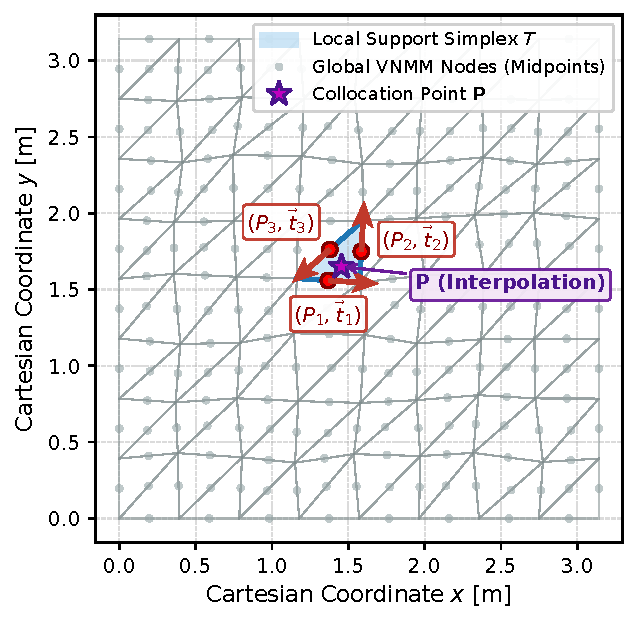
\includegraphics[width=0.52\linewidth]{figura_malha_conforme_vnmm_L1.pdf}
    \caption{Conforming dual topology for Whitney EFEM and VNMM $\mathcal{L}^1$ over $\Omega = [0, \pi]^2$. Underlying triangular mesh overlaid with dual vector nodes placed at edge midpoints $M_k$ with tangent directors $\vec{t}_k$.}
    \label{fig:malha_conforme_vnmm_L1}
\end{figure}

\subsubsection{Numerical Identity and Asymptotic Convergence Rates}
The asymptotic convergence behavior comparing the VNMM 2D $\mathcal{L}^1$ and Whitney EFEM formulations across the seven conforming mesh levels is presented in Fig.~\ref{fig:convergencia_efem_vs_vnmm_L1}.

As demonstrated in Fig.~\ref{fig:convergencia_efem_vs_vnmm_L1}a, the electric field RMS error, defined over the $M$ sampling points as
\begin{equation}
    \|\vec{E} - \vec{E}^h\|_{\mathrm{RMS}} = \sqrt{\frac{1}{M}\sum_{p=1}^M \|\vec{E}(\mathbf{x}_p) - \vec{E}^h(\mathbf{x}_p)\|_2^2},
    \label{eq:rms_error_def}
\end{equation}
displays an identical first-order asymptotic decay rate of $\mathcal{O}(h^{1.00})$ for both formulations. The point-by-point field difference between the two methods remains strictly bounded by double-precision floating-point machine precision, satisfying $\|\vec{E}^{\mathrm{VNMM}} - \vec{E}^{\mathrm{EFEM}}\|_{\mathrm{RMS}} \le 1.6 \times 10^{-16}$.

Similarly, Fig.~\ref{fig:convergencia_efem_vs_vnmm_L1}b illustrates the curl operator RMS error $\|(\nabla \times \vec{E})_z - (\nabla \times \vec{E}^h)_z\|_{\mathrm{RMS}}$, which exhibits an identical fitted convergence rate of $\mathcal{O}(h^{0.96})$ for both formulations. The mutual curl field difference is likewise bounded by machine precision, satisfying $\|(\nabla \times \vec{E})^{\mathrm{VNMM}} - (\nabla \times \vec{E})^{\mathrm{EFEM}}\|_{\mathrm{RMS}} \le 2.5 \times 10^{-15}$. These log-log convergence curves empirically confirm the theoretical demonstration of Theorem~\ref{thm:dual_equivalence} in Section~\ref{subsubsec:formal_proof_dual_whitney}, establishing that under conforming midpoint/tangent placement on triangular cells, the VNMM 2D $\mathcal{L}^1$ formulation and Whitney edge finite elements reproduce identical discrete approximations down to double-precision floating-point roundoff.

\begin{figure}[!htbp]
    \centering
    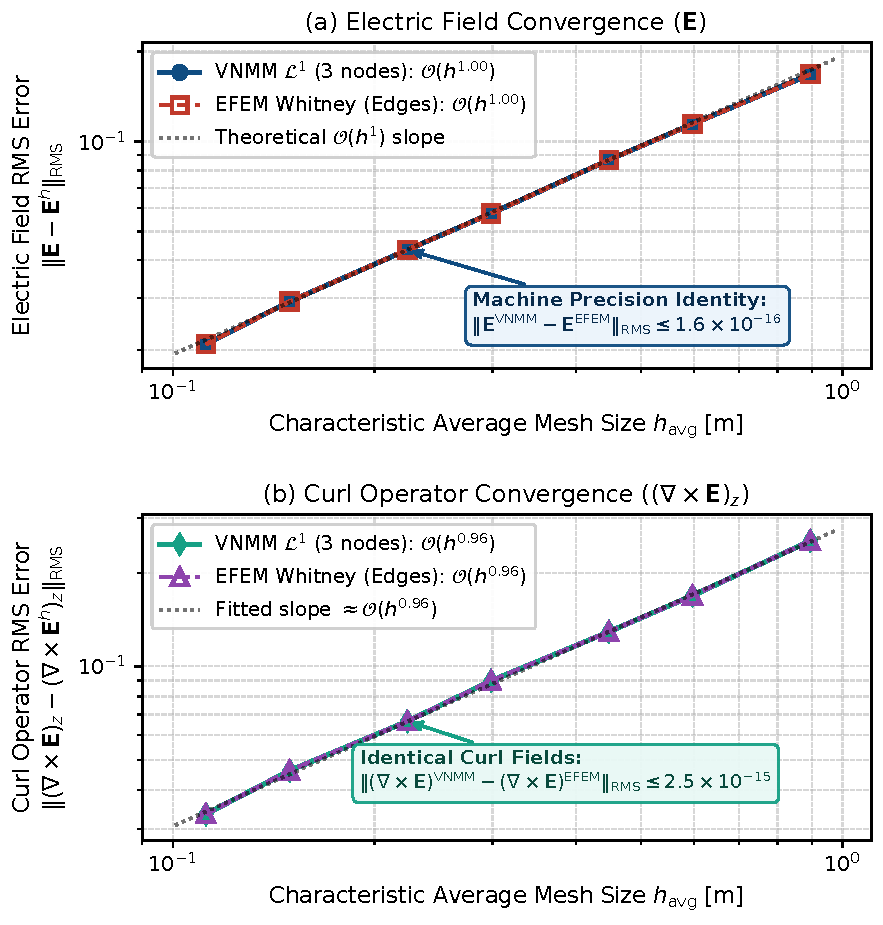
\includegraphics[width=0.62\linewidth]{figura_convergencia_efem_vs_vnmm_L1.pdf}
    \caption{Convergence comparison between Whitney EFEM and VNMM $\mathcal{L}^1$ on conforming triangular meshes.
        (a) Electric field RMS error $\|\vec{E} - \vec{E}^h\|_{\mathrm{RMS}}$ showing identical $\mathcal{O}(h^{1.00})$ convergence;
        (b) Curl operator RMS error displaying identical $\mathcal{O}(h^{0.96})$ convergence down to machine precision, confirming numerical identity.}
    \label{fig:convergencia_efem_vs_vnmm_L1}
\end{figure}

It should be emphasized that this machine-precision equivalence holds strictly under conforming cell topologies where support triads match element midpoints with edge-tangent directors. On arbitrary point clouds, the VNMM ceases to be equivalent to a Whitney element, as arbitrary node coordinates, non-tangential director orientations, and dynamically shifting support stencils destroy simplex conformity, leading to the derivative stagnation examined next.


\subsection{Vector Field Interpolation and Derivative Convergence in Arbitrary Meshless Clouds}
\label{subsec:arbitrary_meshless_interpolation}

To evaluate performance in practical meshless settings where nodes do not coincide with triangulation midpoints, we assess convergence across unconstrained point distributions. This validates the modal aliasing analysis of Section~\ref{subsec:L1_aliasing_analysis} and confirms its resolution through the complete linear space $\mathcal{P}^1$.
\subsubsection{Experimental Setup on Unconstrained Point Clouds}
The interpolation performance is assessed for the analytical $TE_{11}$ cavity mode specified in Eq.~\eqref{eq:analytical_te11_field} over unstructured, non-conforming nodal distributions covering $\Omega = [0, \pi] \times [0, \pi]$. Boundary nodes are placed uniformly along the domain perimeter with counterclockwise unit tangent vectors, whereas internal nodes are generated via a stratified Cartesian grid with $25\%$ stochastic spatial perturbation (\textit{jitter}) and random directional vector orientations $\vec{t}_k = [\cos\theta_k, \sin\theta_k]^T$, where each angle $\theta_k$ is sampled independently from a uniform distribution over the interval $[0, 2\pi)$ ($\theta_k \sim \mathcal{U}(0, 2\pi)$).

To ensure spatial evaluation consistency, all field and derivative errors are evaluated across a fixed, invariant Cartesian grid of $1{,}600$ internal sampling points ($40 \times 40$) distributed uniformly in $[0.04\pi, 0.96\pi]^2$. The computational domain is discretized over six refinement levels, with total node counts $N_{\mathrm{total}} \in \{84, 186, 416, 884, 1{,}928, 4{,}192\}$ and nominal unperturbed boundary spacings ranging from $h_{\mathrm{nom}} = 4\pi / N_{\mathrm{bnd}} = 0.5236$~m down to $0.0654$~m ($h_{\mathrm{nom}} \in \{0.52, 0.35, 0.22, 0.15, 0.10, 0.07\}$~m), where $N_{\mathrm{bnd}} \in \{24, 36, 56, 84, 128, 192\}$ denotes the number of boundary nodes along the perimeter $\partial\Omega$ of length $4\pi$.

\subsubsection{Empirical Validation of Curl Stagnation in \texorpdfstring{$\mathcal{L}^1$}{L1}}
When evaluated on unconstrained meshless clouds, the 3-node solenoidal basis $\mathcal{L}^1$ exhibits the fundamental breakdown in derivative convergence predicted theoretically in Section~\ref{subsec:L1_aliasing_analysis}. As illustrated by the log-log curves in Fig.~\ref{fig:convergencia_interpolacao_L1_vs_P1}a, the electric field RMS error $\|\vec{E} - \vec{E}^h\|_{\mathrm{RMS}}$ under $\mathcal{L}^1$ decreases monotonically at a first-order rate of $\mathcal{O}(h^{0.97})$, dropping from $1.91 \times 10^{-1}$ ($h_{\mathrm{nom}} = 0.5236$~m) down to $2.46 \times 10^{-2}$ ($h_{\mathrm{nom}} = 0.0654$~m).

However, as revealed in Fig.~\ref{fig:convergencia_interpolacao_L1_vs_P1}b, the RMS error of the curl operator $\|(\nabla \times \vec{E})_z - (\nabla \times \vec{E}^h)_z\|_{\mathrm{RMS}}$ \textbf{stagnates at an $\mathcal{O}(1)$ error plateau} ($\approx 0.85$, varying between $8.33 \times 10^{-1}$ and $8.88 \times 10^{-1}$, asymptotic rate $\mathcal{O}(h^{-0.01}) \approx \mathcal{O}(1)$), failing to converge under spatial refinement ($N_{\mathrm{total}} = 4{,}192$). This persistent noise floor confirms the modal aliasing mechanism derived in Section~\ref{subsec:L1_aliasing_analysis}, wherein unrepresented normal field derivatives leak into the rotational coefficient via the inverted placement matrix $\mathbf{A}^{-1}$.
\begin{figure}[!htbp]
    \centering
    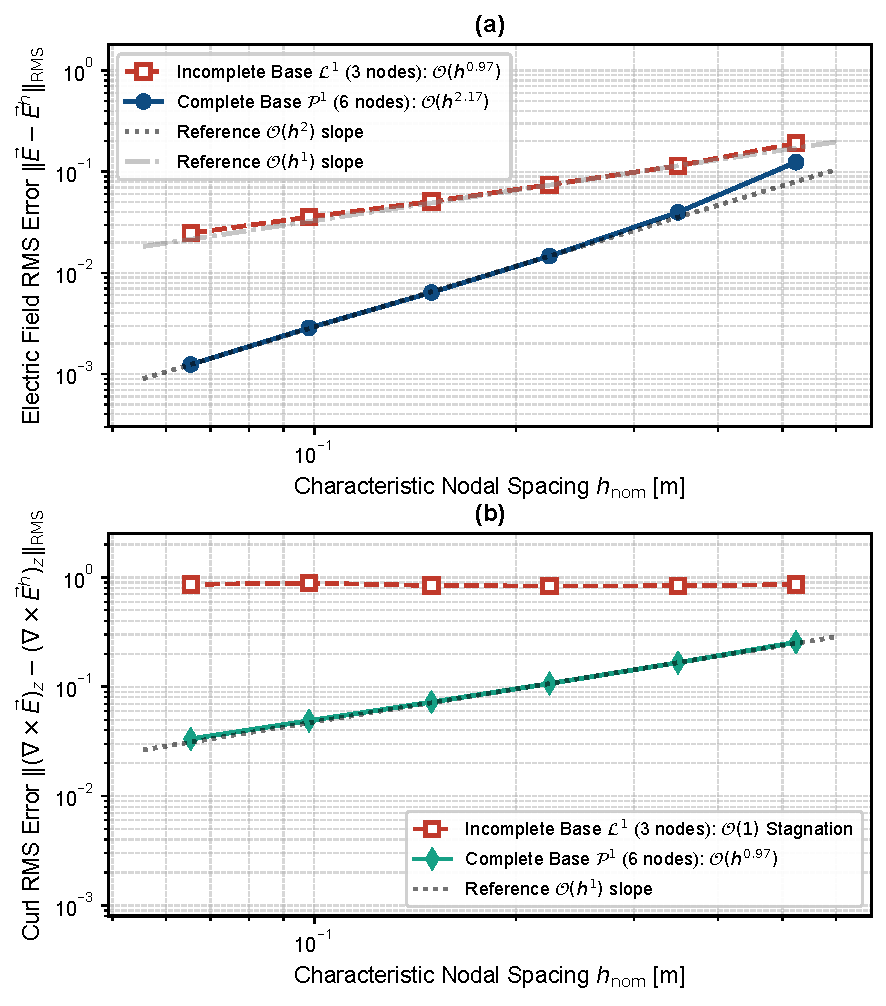
\includegraphics[width=0.62\linewidth]{figura_convergencia_interpolacao_L1_vs_P1.pdf}
    \caption{Convergence of $\mathcal{L}^1$ and $\mathcal{P}^1$ bases on unconstrained point clouds for the $TE_{11}$ mode.
        (a) Electric field RMS error showing $\mathcal{O}(h^{0.97})$ ($\mathcal{L}^1$) versus $\mathcal{O}(h^{2.17})$ ($\mathcal{P}^1$);
        (b) Curl operator RMS error highlighting $\mathcal{O}(1)$ stagnation for $\mathcal{L}^1$ and restored $\mathcal{O}(h^{0.97})$ convergence for $\mathcal{P}^1$.}
    \label{fig:convergencia_interpolacao_L1_vs_P1}
\end{figure}

\subsubsection{Restoration of Asymptotic Convergence via Complete \texorpdfstring{$\mathcal{P}^1$}{P1} Basis}
Expanding the local approximation space to the complete linear polynomial vector space $\mathcal{P}^1$ introduced in Section~\ref{subsec:complete_P1_basis} provides six independent degrees of freedom, capturing all four components of the local Jacobian tensor $\nabla\vec{E}^h$. Local support domains (averaging $K_{\mathrm{avg}} \approx 11.0$ neighbors, ranging from $10.7$ to $11.2$) are selected via $k$-d tree spatial searches subject to the scale-invariant dimensionless determinant threshold developed in Section~\ref{sec:support_selection_algorithm}, evaluated with the normalization scale set to the nominal spacing $h_{\mathrm{local}} = h_{\mathrm{nom}}$ and operating at the calibrated dimensionless threshold $\widehat{\mathrm{Tol}} = 0.80$.

As demonstrated in Fig.~\ref{fig:convergencia_interpolacao_L1_vs_P1}, transitioning to $\mathcal{P}^1$ removes derivative modal aliasing and achieves two major performance gains:
\begin{enumerate}
    \item \textbf{Observed Convergence for Field $\vec{E}^h$ (Fig.~\ref{fig:convergencia_interpolacao_L1_vs_P1}a):} Completing the linear polynomial space elevates the observed electric field convergence rate from $\mathcal{O}(h^{0.97})$ under $\mathcal{L}^1$ to an observed fitted slope of $\mathcal{O}(h^{2.17})$ under $\mathcal{P}^1$. At the finest discretization ($h_{\mathrm{nom}} = 0.0654$~m), the field RMS error drops from $2.46 \times 10^{-2}$ ($\mathcal{L}^1$) down to $1.24 \times 10^{-3}$ ($\mathcal{P}^1$), representing a \textbf{$19.8\times$ precision gain}. This empirical convergence acceleration highlights the substantial accuracy benefit of resolving the complete local Jacobian, in contrast to the incomplete $\mathcal{L}^1$ formulation whose missing longitudinal polynomial terms restrict error reduction.
    \item \textbf{Restoration of Asymptotic $\mathcal{O}(h^1)$ Curl Convergence (Fig.~\ref{fig:convergencia_interpolacao_L1_vs_P1}b):} By accommodating normal derivatives in the Taylor expansion, the complete $\mathcal{P}^1$ basis restores first-order convergence $\mathcal{O}(h^{0.97})$ for the curl operator. The curl RMS error decreases monotonically from $2.55 \times 10^{-1}$ down to $3.33 \times 10^{-2}$ at $h_{\mathrm{nom}} = 0.0654$~m, delivering a \textbf{$25.9\times$ error reduction} over the stagnated $\mathcal{L}^1$ formulation ($8.63 \times 10^{-1}$).
\end{enumerate}

Consequently, while $\mathcal{L}^1$ is suitable for conforming triangular meshes where circulation cancellation holds (Section~\ref{subsec:conforming_dual_equivalence}), adopting the complete $\mathcal{P}^1$ vector space is sufficient to eliminate the derivative-aliasing mechanism and restore first-order curl convergence across unconstrained, arbitrary meshless point clouds. The quantitative performance comparison between the two bases across all six refinement levels is detailed in Table~\ref{tab:interpolacao_L1_vs_P1}.

\begin{table}[!htbp]
    \centering
    \caption{Comparative interpolation and curl error metrics between $\mathcal{L}^1$ and $\mathcal{P}^1$ bases on perturbed point clouds for the $TE_{11}$ mode across six refinement levels.}
    \label{tab:interpolacao_L1_vs_P1}
    \resizebox{\columnwidth}{!}{%
        \begin{tabular}{@{} c c c c c c c c c @{}}
            \toprule
            $N_{\mathrm{total}}$                     & $h_{\mathrm{nom}}$ [m]  & \multicolumn{3}{c}{\textbf{Electric Field RMS Error}} & \multicolumn{3}{c}{\textbf{Curl Operator RMS Error}} & $K_{\mathrm{avg}}$                                                                                                              \\
            \cmidrule(lr){3-5} \cmidrule(lr){6-8}
                                                     &                         & $\mathcal{L}^1$                                       & $\mathcal{P}^1$                                      & \textbf{Gain}            & $\mathcal{L}^1$                  & $\mathcal{P}^1$       & \textbf{Gain}         & ($\mathcal{P}^1$) \\
            \midrule
            84                                       & 0.5236                  & $1.91 \times 10^{-1}$                                 & $1.24 \times 10^{-1}$                                & $\mathbf{1.5\times}$     & $8.61 \times 10^{-1}$            & $2.55 \times 10^{-1}$ & $\mathbf{3.4\times}$  & 11.1              \\
            186                                      & 0.3491                  & $1.15 \times 10^{-1}$                                 & $3.97 \times 10^{-2}$                                & $\mathbf{2.9\times}$     & $8.38 \times 10^{-1}$            & $1.66 \times 10^{-1}$ & $\mathbf{5.0\times}$  & 11.2              \\
            416                                      & 0.2244                  & $7.44 \times 10^{-2}$                                 & $1.47 \times 10^{-2}$                                & $\mathbf{5.1\times}$     & $8.34 \times 10^{-1}$            & $1.07 \times 10^{-1}$ & $\mathbf{7.8\times}$  & 11.2              \\
            884                                      & 0.1496                  & $5.08 \times 10^{-2}$                                 & $6.39 \times 10^{-3}$                                & $\mathbf{7.9\times}$     & $8.43 \times 10^{-1}$            & $7.24 \times 10^{-2}$ & $\mathbf{11.6\times}$ & 10.9              \\
            1{,}928                                  & 0.0982                  & $3.56 \times 10^{-2}$                                 & $2.86 \times 10^{-3}$                                & $\mathbf{12.5\times}$    & $8.88 \times 10^{-1}$            & $4.89 \times 10^{-2}$ & $\mathbf{18.1\times}$ & 10.9              \\
            4{,}192                                  & 0.0654                  & $2.46 \times 10^{-2}$                                 & $1.24 \times 10^{-3}$                                & $\mathbf{19.8\times}$    & $8.63 \times 10^{-1}$            & $3.33 \times 10^{-2}$ & $\mathbf{25.9\times}$ & 10.7              \\
            \midrule
            \multicolumn{2}{c}{\textbf{Fitted Rate}} & $\mathcal{O}(h^{0.97})$ & $\mathbf{\mathcal{O}(h^{2.17})}$                      & ---                                                  & $\mathcal{O}(h^{-0.01})$ & $\mathbf{\mathcal{O}(h^{0.97})}$ & ---                   & ---                                       \\
            \bottomrule
        \end{tabular}%
    }
\end{table}

% ---------------------------------------------------------
% SUBSECTION 5.3: NUMERICAL STABILITY UNDER STOCHASTIC PERTURBATIONS
% ---------------------------------------------------------
\subsection{Numerical Robustness in the Tested Stochastic Realization Under Spatial-Directional Perturbations}
\label{subsec:stochastic_perturbations}

While the benchmark in Section~\ref{subsec:arbitrary_meshless_interpolation} adopted a fixed, calibrated threshold ($\widehat{\mathrm{Tol}} = 0.80$) to demonstrate the restoration of asymptotic convergence via the complete $\mathcal{P}^1$ basis, it did not examine how the choice of $\widehat{\mathrm{Tol}}$ itself governs stencil qualification. On unconstrained point clouds with spatial and directional disorder, arbitrary node-director arrangements can induce localized geometric pathologies (such as clusters of near-parallel directors or near-collinear nodes; Section~\ref{subsec:singularities_P1}) that severely degrade the conditioning of the local placement matrix $\mathbf{A} \in \mathbb{R}^{6 \times 6}$. Retaining the exact same stochastically perturbed point cloud sequence ($25\%$ spatial jitter and uniform random director orientations $\theta_k \sim \mathcal{U}(0, 2\pi)$ across $N_{\mathrm{total}} = 84$ to $4{,}192$), this section systematically investigates how the value of $\widehat{\mathrm{Tol}}$ influences algebraic stability, support size, and solution accuracy, addressing two concrete objectives:
\begin{enumerate}
    \item \textbf{Demonstration of Numerical Degradation Under Permissive Support Filtering:} Analyze the failure mechanism that occurs when an overly relaxed selection threshold is used ($\widehat{\mathrm{Tol}} \le 0.05$), showing how accepting ill-conditioned immediate neighbor sextets inflates the condition number ($\kappa_2(\widehat{\mathbf{A}}) > 13$, unscaled $\kappa_2(\mathbf{A}) > 180$) and degrades fine-mesh derivative convergence.
    \item \textbf{Parametric Robustness and Operating Window of $\widehat{\mathrm{Tol}}$:} Demonstrate that the scale-invariant threshold criterion $|\det(\widehat{\mathbf{A}})| \ge \widehat{\mathrm{Tol}}$ (Eq.~\eqref{eq:dimensionless_threshold_criterion}) reliably detects and filters degenerate configurations, empirically bounding placement matrix conditioning ($\kappa_2(\widehat{\mathbf{A}}) \le 5.9$) while preserving compact local supports ($K_{\mathrm{avg}} \approx 10\text{--}11$), and conduct a systematic parametric sweep over $\widehat{\mathrm{Tol}} \in [0.05, 6.00]$ on the finest point cloud ($N_{\mathrm{total}} = 4{,}192$) to identify the optimal operating regime for the 2D VNMM.
\end{enumerate}

Although extensive Monte Carlo characterization across multi-seed ensembles remains future work, this single-realization sequence provides a representative stress test for the automated qualification pipeline, assessing whether the scale-invariant determinant threshold can dynamically detect and bypass localized pathological candidate sextets without manual intervention. Figure~\ref{fig:robustez_perturbacao_estocastica} and Table~\ref{tab:stochastic_sensitivity_ultradense} summarize the resulting convergence behavior, placement matrix conditioning, and parametric sensitivity analysis for this benchmark sequence.

\begin{figure}[!htbp]
    \centering
    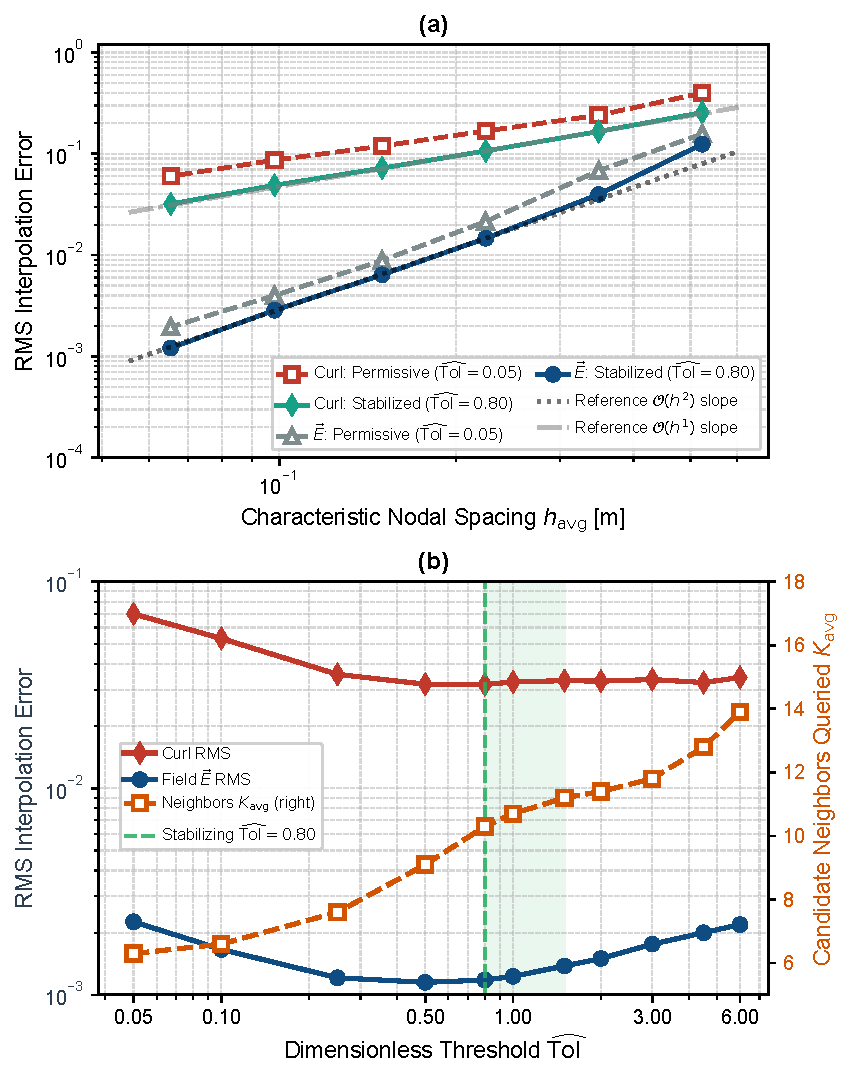
\includegraphics[width=0.62\linewidth]{figura_robustez_perturbacao_estocastica.pdf}
    \caption{Conditioning and robustness of the VNMM $\mathcal{P}^1$ basis under spatial-directional perturbations.
    (a) Electric field and curl RMS errors versus nominal spacing $h_{\mathrm{nom}}$, comparing a permissive threshold ($\widehat{\mathrm{Tol}} = 0.05$) against the calibrated threshold ($\widehat{\mathrm{Tol}} = 0.80$);
    (b) Error metrics and average support size $K_{\mathrm{avg}}$ versus $\widehat{\mathrm{Tol}}$ on the fine cloud ($N_{\mathrm{total}} = 4{,}192$), identifying the stable window $\widehat{\mathrm{Tol}} \in [0.80, 1.50]$.}
    \label{fig:robustez_perturbacao_estocastica}
\end{figure}

\subsubsection{Degradation Under Overly Permissive Thresholds (\texorpdfstring{$\widehat{\mathrm{Tol}} \ll 1$}{Tol << 1})}
\label{subsubsec:permissive_threshold_degradation}

To demonstrate the critical role of scale-invariant support filtering, we first examine the behavior of the qualification algorithm when an excessively relaxed dimensionless threshold is applied (e.g., $\widehat{\mathrm{Tol}} \le 0.05$).

Under stochastic spatial-directional noise, an overly permissive threshold causes numerical stagnation:
\begin{itemize}
    \item At $\widehat{\mathrm{Tol}} \le 0.05$, the early-stopping qualification accepts the immediate 6 nearest spatial neighbors ($K_{\mathrm{avg}} \approx 6.3$).
    \item Because node coordinates and directors are stochastically perturbed, these immediate spatial neighbors frequently form ill-conditioned sextets approaching the singularity modes analyzed in Section~\ref{subsec:singularities_P1} (such as 4 near-parallel directors or 5 near-collinear nodes), elevating the intrinsic condition number to $\kappa_2(\widehat{\mathbf{A}}) > 13$ (corresponding to unscaled $\kappa_2(\mathbf{A}) > 180$).
    \item Because spatial derivatives scale analytically as $\mathcal{O}(h^{-1})$ via Eq.~\eqref{eq:curl_hat_eval}, the ill-conditioned inverted matrix $\widehat{\mathbf{A}}^{-1}$ amplifies local projection errors. As shown by the dashed crimson curve in Fig.~\ref{fig:robustez_perturbacao_estocastica}a, this causes the curl operator RMS error to flatten and stagnate as $h_{\mathrm{nom}} \to 0.0654$~m, remaining elevated at an RMS error plateau of $\approx 6.01 \times 10^{-2}$ to $8.66 \times 10^{-2}$ for $(\nabla \times \vec{E}^h)_z$.
\end{itemize}

\subsubsection{Restoration of Monotonic Convergence via Scale-Invariant Thresholding}
\label{subsubsec:restoration_via_thresholding}

Enforcing a scale-invariant lower bound $\widehat{\mathrm{Tol}} \ge 0.80$ completely eliminates this derivative instability.

As demonstrated by the solid curves (teal for curl and navy for field) in Fig.~\ref{fig:robustez_perturbacao_estocastica}a, requiring $|\det(\widehat{\mathbf{A}})| \ge 0.80$ systematically rejects candidate sextets afflicted by directional parallelism or near-collinear alignments. This prompts the candidate search to expand its local sampling radius moderately ($K_{\mathrm{avg}}$ expands from $6.3$ to $10.3$), automatically identifying well-conditioned support sextets with balanced angular diversity. By dynamically identifying an admissible support via the 4-phase selection algorithm (Section~\ref{subsec:4phase_pipeline}), the method restores strict monotonic error reduction across the tested refinement range for both field $\vec{E}^h$ and curl $(\nabla \times \vec{E}^h)_z$, reducing fine-mesh curl error to $3.18 \times 10^{-2}$ on $N_{\mathrm{total}} = 4{,}192$.

Because this criterion is formulated directly on the dimensionless placement matrix $\widehat{\mathbf{A}}$, the threshold $\widehat{\mathrm{Tol}}$ is intrinsically scale-invariant across all refinement levels. Unlike any dimensional determinant threshold, which decays as $\mathcal{O}(h^4)$ under grid refinement, the dimensionless criterion preserves compact supports ($K_{\mathrm{avg}} \approx 6.0$ on regular grids, $K_{\mathrm{avg}} \approx 10\text{--}11$ on perturbed clouds) down to arbitrarily fine grid scales.

\subsubsection{Parametric Neighborhood Trade-off and Stable Operating Window}
\label{subsubsec:parametric_tradeoff}

To identify the best-performing compromise between conditioning, curl error, and neighborhood size on $\Omega = [0, \pi]^2$, a systematic parametric sweep was conducted on the stochastically perturbed fine point cloud ($N_{\mathrm{total}} = 4{,}192, h_{\mathrm{nom}} = 0.0654$~m) across clean, round dimensionless thresholds ranging from $\widehat{\mathrm{Tol}} = 0.05$ up to $\widehat{\mathrm{Tol}} = 6.00$. Following the uniform convention $h_{\mathrm{local}} = h_{\mathrm{nom}}$ established in Section~\ref{sec:numerical_results} and the point-cloud sequence of Section~\ref{subsec:arbitrary_meshless_interpolation}, the nominal characteristic spacing on this fine point cloud ($N_{\mathrm{total}} = 4{,}192$) is $h_{\mathrm{nom}} = 0.0654$~m ($N_{\mathrm{bnd}} = 192$) across all evaluation points, guaranteeing exact numerical reproducibility of the placement matrices. Notably, support domain determinations were executed with total success across all tested thresholds ($\widehat{\mathrm{Tol}} \in [0.05, 6.00]$): in every case, $100\%$ of the $1{,}600$ evaluation points identified an admissible support sextet without encountering search starvation or requiring fallback procedures. As discussed in Section~\ref{subsec:scale_invariant_criterion}, because a lower bound on the determinant does not mathematically control the condition number without a bounded proximity hypothesis ($\|\hat{\mathbf{x}}_k\| \le C$), Table~\ref{tab:stochastic_sensitivity_ultradense} provides the direct empirical qualification data evaluating $|\det(\widehat{\mathbf{A}})|$ versus $\kappa_2(\widehat{\mathbf{A}})$: it systematically reports how varying the threshold criterion $|\det(\widehat{\mathbf{A}})| \ge \widehat{\mathrm{Tol}}$ influences the candidate query size $K_{\mathrm{avg}}$, the condition number $\kappa_2(\widehat{\mathbf{A}})$ (and unscaled $\kappa_2(\mathbf{A})$), and the resulting interpolation errors.

\begin{table}[!htbp]
    \centering
    \caption{Sensitivity of error metrics, support neighborhood $K_{\mathrm{avg}}$, and conditioning to the dimensionless threshold $\widehat{\mathrm{Tol}}$ on the fine point cloud ($N_{\mathrm{total}} = 4{,}192$).}
    \label{tab:stochastic_sensitivity_ultradense}
    \resizebox{\columnwidth}{!}{%
        \begin{tabular}{@{} c c c c c @{}}
            \toprule
            \textbf{Dimensionless Threshold}                                                            & \textbf{Neighbors} & \multicolumn{2}{c}{\textbf{RMS Error}} & \textbf{Conditioning}                                                                                                                     \\
            \cmidrule(lr){3-4}
            $\widehat{\mathrm{Tol}}$                                                                    & $K_{\mathrm{avg}}$ & $\vec{E}^h$                            & $(\nabla\times\vec{E}^h)_z$    & $\kappa_2(\widehat{\mathbf{A}}) \; [\kappa_2(\mathbf{A})]$                                               \\
            \midrule
            \begin{tabular}[c]{@{}c@{}} 0.05 \\ \scriptsize(Permissive) \end{tabular}                   & 6.3                & $2.26 \times 10^{-3}$                  & $6.98 \times 10^{-2}$          & \begin{tabular}[c]{@{}c@{}} $\approx 13.4 \; [186]$ \\ \scriptsize(Ill-cond.) \end{tabular}              \\
            0.10                                                                                        & 6.6                & $1.66 \times 10^{-3}$                  & $5.31 \times 10^{-2}$          & $\approx 11.8 \; [162]$                                                                                  \\
            0.25                                                                                        & 7.6                & $1.21 \times 10^{-3}$                  & $3.56 \times 10^{-2}$          & $\approx 9.0 \; [124]$                                                                                   \\
            0.50                                                                                        & 9.1                & $1.15 \times 10^{-3}$                  & $3.19 \times 10^{-2}$          & $\approx 6.9 \; [94]$                                                                                    \\
            \begin{tabular}[c]{@{}c@{}} \textbf{0.80} \\ \scriptsize\textbf{(Stable)} \end{tabular}     & \textbf{10.3}      & $\mathbf{1.18 \times 10^{-3}}$         & $\mathbf{3.18 \times 10^{-2}}$ & \begin{tabular}[c]{@{}c@{}} $\mathbf{\approx 5.9 \; [80]}$ \\ \scriptsize\textbf{(Stable)} \end{tabular} \\
            1.00                                                                                        & 10.7               & $1.23 \times 10^{-3}$                  & $3.27 \times 10^{-2}$          & $\approx 5.6 \; [75]$                                                                                    \\
            \begin{tabular}[c]{@{}c@{}} \textbf{1.50} \\ \scriptsize\textbf{(Compromise)} \end{tabular} & \textbf{11.2}      & $\mathbf{1.38 \times 10^{-3}}$         & $\mathbf{3.32 \times 10^{-2}}$ & \begin{tabular}[c]{@{}c@{}} $\mathbf{\approx 5.1 \; [66]}$ \\ \scriptsize\textbf{(Stable)} \end{tabular} \\
            2.00                                                                                        & 11.4               & $1.50 \times 10^{-3}$                  & $3.30 \times 10^{-2}$          & $\approx 4.6 \; [59]$                                                                                    \\
            3.00                                                                                        & 11.8               & $1.76 \times 10^{-3}$                  & $3.36 \times 10^{-2}$          & $\approx 4.0 \; [50]$                                                                                    \\
            \begin{tabular}[c]{@{}c@{}} 6.00 \\ \scriptsize(Over-constrained) \end{tabular}             & 13.9               & $2.19 \times 10^{-3}$                  & $3.44 \times 10^{-2}$          & $\approx 3.3 \; [39]$                                                                                    \\
            \bottomrule
        \end{tabular}%
    }
\end{table}

As illustrated in Fig.~\ref{fig:robustez_perturbacao_estocastica}b:
\begin{enumerate}
    \item \textbf{Stabilization Zone ($\widehat{\mathrm{Tol}} \ge 0.80$):} Increasing $\widehat{\mathrm{Tol}}$ from $0.05$ to $0.80$ produces a sharp, monotonic reduction in curl interpolation error (a $2.2\times$ precision gain from $6.98 \times 10^{-2}$ down to $3.18 \times 10^{-2}$), while bounding the intrinsic dimensionless conditioning to $\kappa_2(\widehat{\mathbf{A}}) \le 5.9$ (unscaled $\kappa_2(\mathbf{A}) \le 80$) and decreasing to $\kappa_2(\widehat{\mathbf{A}}) \approx 5.1$ at the compromise threshold $\widehat{\mathrm{Tol}} = 1.50$.
    \item \textbf{Compact Support Locality and Trade-off ($K_{\mathrm{avg}} \le 11.2$):} This precision gain requires expanding the candidate search neighborhood from $K_{\mathrm{avg}} = 6.3$ to only $K_{\mathrm{avg}} = 10.3$ (at $\widehat{\mathrm{Tol}} = 0.80$) and $11.2$ (at the compromise threshold $\widehat{\mathrm{Tol}} = 1.50$). While larger thresholds ($\widehat{\mathrm{Tol}} \ge 3.00$) further reduce $\kappa_2(\widehat{\mathbf{A}})$ to $\approx 3.3\text{--}4.0$, they do so at the cost of wider candidate search pools ($K_{\mathrm{avg}} \to 13.9$ at $\widehat{\mathrm{Tol}} = 6.00$) and elevated field interpolation errors ($2.19 \times 10^{-3}$ vs. $1.18 \times 10^{-3}$, an $85\%$ increase), establishing $\widehat{\mathrm{Tol}} \in [0.80, 1.50]$ as the best-performing compromise between conditioning, curl error, and neighborhood size. Significantly, this compact neighborhood size matches that of unperturbed clouds ($K_{\mathrm{avg}} \approx 11.0$, Table~\ref{tab:interpolacao_L1_vs_P1}), demonstrating that scale-invariant thresholding effectively suppresses directional collinearities without scale-induced support dilation, thereby preserving spatial search efficiency and compact support locality without combinatorial overhead (Section~\ref{subsubsec:computational_complexity}).
\end{enumerate}

In summary, this benchmark confirms the mechanical efficacy of scale-invariant thresholding in preventing derivative stagnation across perturbed point clouds with arbitrary director orientations.


% ---------------------------------------------------------
% SUBSECTION 5.4: RESONANT CAVITY SPECTRAL ANALYSIS AND DIV-CURL REGULARIZATION
% ---------------------------------------------------------
\subsection{Spectral Validation: Resonant Cavity Analysis and Div-Curl Regularization}
\label{subsec:cavity_eigenvalues}
Having established the variational framework for the electromagnetic vector eigenvalue problem in Section~\ref{sec:variational_formulation}, this experiment evaluates the spectral accuracy of the Vector Nodal Meshless Method and verifies the suppression of non-physical spurious modes across the operational frequency band. Numerical simulations are conducted for Transverse Electric ($TE_z$) modes over the square PEC cavity using the complete $\mathcal{P}^1$ basis, comparing discrete spectra against the analytical reference eigenvalues defined in Eq.~\eqref{eq:analytical_eigenvalues}.

Numerical evaluations are conducted on the base-case discretization with $N_x = 21, N_y = 21$ ($N_{\mathrm{total}} = 441$ nodes, yielding $N_{\mathrm{DoF}} = (N_x - 2)^2 = 361$ active internal degrees of freedom after enforcing homogeneous tangential PEC boundary conditions $e_k = 0$ on $\partial\Omega$). Over the domain $\Omega = [0, L_x] \times [0, L_y] = [0, \pi]^2$, the nominal characteristic nodal spacing is defined as $h_{\mathrm{nom}} = \frac{L_x}{N_x - 1} = \frac{\pi}{20} \approx 0.1571$~m. Interior nodes are placed on a regular Cartesian grid:
\begin{equation}
    \mathbf{x}_{i,j} = \left(i \, h_{\mathrm{nom}}, \; j \, h_{\mathrm{nom}}\right), \quad i = 1, \dots, N_x - 2, \quad j = 1, \dots, N_y - 2.
    \label{eq:regular_grid_coords}
\end{equation}
To eliminate geometric director ambiguity at sharp $90^\circ$ corners and prevent corner node starvation, boundary nodes are generated via a \textbf{staggered face-centered distribution} (centered at subsegment midpoints along each wall, consistent with the methodology of Sections~\ref{subsec:arbitrary_meshless_interpolation} and~\ref{subsec:stochastic_perturbations}), placing $N_x - 1 = 20$ nodes along each of the four walls ($N_{\mathrm{bnd}} = 80$ boundary nodes, preserving $N_{\mathrm{total}} = 441$):
\begin{align}
    \text{Horizontal walls } (y \in \{0, L_y\}): \quad & \mathbf{x}_k = \left( \left(k + \frac{1}{2}\right) h_{\mathrm{nom}}, \; y \right), \quad \vec{t}_k = \begin{bmatrix} 1 \\ 0 \end{bmatrix}, \label{eq:staggered_bnd_horiz} \\
    \text{Vertical walls } (x \in \{0, L_x\}): \quad   & \mathbf{x}_k = \left( x, \; \left(k + \frac{1}{2}\right) h_{\mathrm{nom}} \right), \quad \vec{t}_k = \begin{bmatrix} 0 \\ 1 \end{bmatrix}, \label{eq:staggered_bnd_vert}
\end{align}
for $k = 0, \dots, N_x - 2$. By construction, this staggered placement ensures that all boundary nodes lie strictly in the open interior of each domain edge, maintaining a distance of at least $\frac{h_{\mathrm{nom}}}{2} = \frac{\pi}{40} \approx 0.0785$~m from every corner $(0,0), (\pi,0), (0,\pi), (\pi,\pi)$, completely freeing the four cavity vertices from co-located nodal degrees of freedom. Homogeneous tangential PEC boundary conditions ($\vec{E}^h(\mathbf{x}_k) \cdot \vec{t}_k = 0$) are enforced via nodal elimination ($e_k = 0$).

For interior nodes ($i \in \{1, \dots, N_x-2\}$, $j \in \{1, \dots, N_y-2\}$), unit director vectors $\vec{t}_{i,j}$ are assigned following an alternating orientation pattern, governed by the exact mathematical rule:
\begin{equation}
    \vec{t}_{i,j} = \begin{cases}
        \begin{bmatrix} \cos(45^\circ) \\ \sin(45^\circ) \end{bmatrix} = \begin{bmatrix} \frac{\sqrt{2}}{2} \\ \frac{\sqrt{2}}{2} \end{bmatrix},      & \text{if } (i + j) \text{ is even}, \\[10pt]
        \begin{bmatrix} \cos(135^\circ) \\ \sin(135^\circ) \end{bmatrix} = \begin{bmatrix} -\frac{\sqrt{2}}{2} \\ \frac{\sqrt{2}}{2} \end{bmatrix}, & \text{if } (i + j) \text{ is odd}.
    \end{cases}
    \label{eq:alternating_directors_def}
\end{equation}
This checkerboard alternating pattern guarantees local orthogonal angular diversity: every internal node is surrounded by nearest neighbors whose assigned directors are mutually orthogonal ($\vec{t}_{45^\circ} \cdot \vec{t}_{135^\circ} = 0$), preventing directional parallelism and ensuring that any candidate 6-node stencil contains balanced projection moments.

The weak form integrals are computed over a background grid of $10 \times 10$ quadrilateral cells ($N_c = 100$) using $2 \times 2$ Gauss-Legendre quadrature (400 Gauss points), maintaining a suitable quadrature-to-DoF ratio ($N_g / N_{\mathrm{DoF}} \approx 1.11$) \cite{belytschko1994element, liu2005introduction, liu2009mesh}. At each Gauss integration point $P_g$, active support sextets are determined via the scale-invariant qualification criterion $|\det(\widehat{\mathbf{A}})| \ge \widehat{\mathrm{Tol}}$ (Section~\ref{subsec:scale_invariant_criterion}), with the local normalization scale set to the nominal spacing $h_{\mathrm{local}} = h_{\mathrm{nom}} = 0.1571$~m (Section~\ref{sec:numerical_results}) and the threshold set to the stabilized operating value $\widehat{\mathrm{Tol}} = 0.80$ identified in Section~\ref{subsec:stochastic_perturbations}. On this structured lattice with the alternating unit directors defined in Eq.~\eqref{eq:alternating_directors_def}, the geometric symmetry and orthogonal angular diversity of immediate neighbors generate well-conditioned placement matrices across all 400 quadrature points (mean $|\det(\widehat{\mathbf{A}})| \approx 3.43$). Consequently, the selection algorithm identifies compact nearest-neighbor stencils ($K_{\mathrm{avg}} = 6.99 \approx 7.00$) without support dilation, ensuring that the discrete system matrices $\mathbf{K}$ and $\mathbf{M}$ remain identically invariant across the entire stable threshold range $\widehat{\mathrm{Tol}} \le 1.00$ (such as $\widehat{\mathrm{Tol}} \in [0.10, 0.80]$).

\subsubsection{Spectral Contamination in the Unregularized Curl-Curl Formulation (\texorpdfstring{$s_{\mathrm{div}} = 0.0$}{s(div) = 0.0})}
\label{subsubsec:unregularized_formulation}

As established in Section~\ref{subsec:weak_form_regularization}, unregularized meshless discretizations lack discrete de Rham exactness, allowing discrete gradient fields to produce non-vanishing numerical curl residues ($\nabla_h \times \nabla_h \phi_h \neq \mathbf{0}$) at Gauss quadrature points.

Importantly, the algebraic structure of the unregularized operator $\mathbf{K}_{\mathrm{curl}}$ demonstrates that this contamination is not an artifact of background quadrature under-integration. In the coarse baseline discretization ($10 \times 10$ cells, $2 \times 2$ Gauss points, $N_g = 400$, $N_g/N_{\mathrm{DoF}} \approx 1.11$), $\mathbf{K}_{\mathrm{curl}}$ exhibits an artificial numerical nullspace of dimension $\dim\ker(\mathbf{K}_{\mathrm{curl}}) = 140$, caused by Gauss points under-sampling the gradient space. However, when the background quadrature is fully refined to node-conforming cells with high-order integration ($20 \times 20$ cells, $3 \times 3$ Gauss points, $N_g = 3600$, $N_g/N_{\mathrm{DoF}} \approx 10.0$), this artificial nullspace vanishes entirely ($\dim\ker(\mathbf{K}_{\mathrm{curl}}) = 0$). Instead of static zero states, the unconstrained discrete gradient subspace leaks completely into the positive spectrum, generating a dense ladder of non-physical spurious eigenvalues $\lambda \in (0.05, 0.90)$ strictly below the fundamental physical resonance ($TE_{10}, \lambda = 1.0$).

The empirical impact of this nullspace leakage is illustrated in Fig.~\ref{fig:espectro_cavidade_regularizacao}a. Without volumetric divergence regularization ($s_{\mathrm{div}} = 0.0$), these non-physical gradient modes densely infiltrate the physical $TE_z$ spectrum, completely corrupting analytical modal ordering and elevating the mean relative cutoff wavenumber error to unacceptable levels ($17.96\%$ in Table~\ref{tab:s_div_sensitivity}, extending above $34\%$ for higher modes).

\begin{figure}[!htbp]
    \centering
    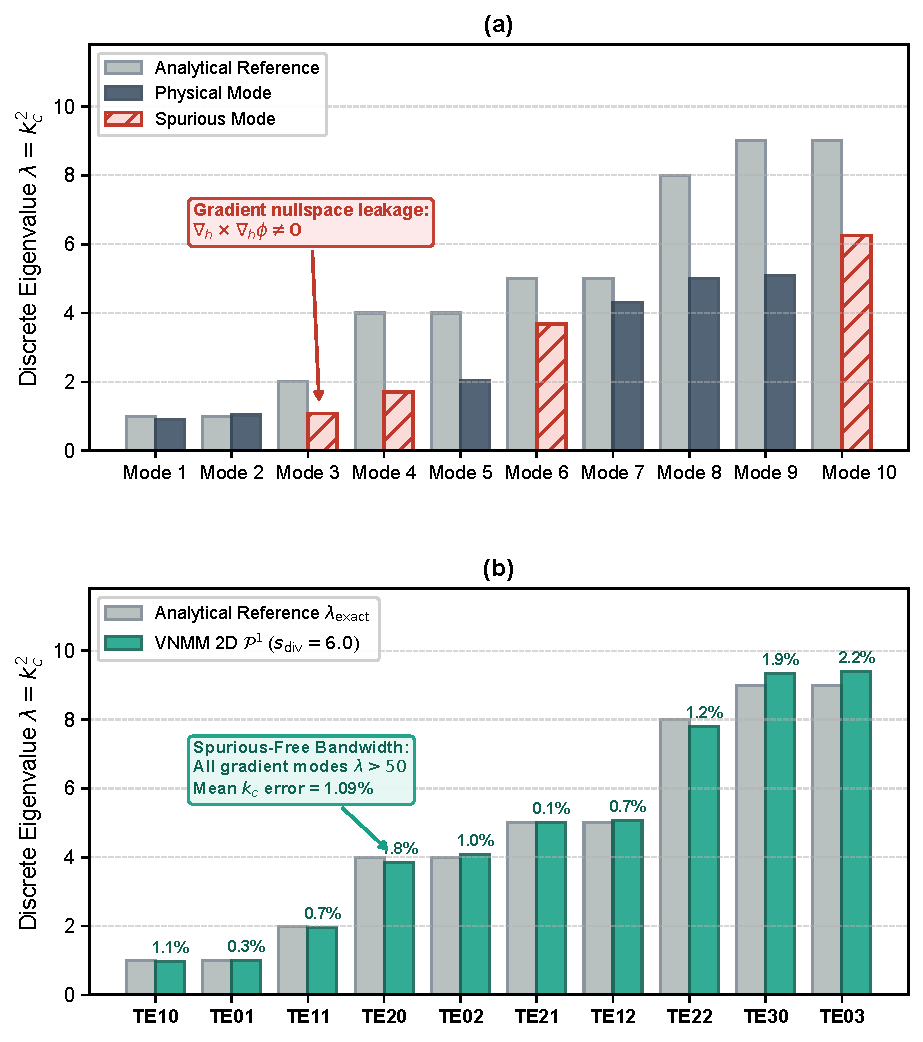
\includegraphics[width=0.62\linewidth]{figura_espectro_cavidade_com_sem_regularizacao.pdf}
    \caption{Discrete eigenvalue spectrum $\lambda = k_c^2$ for the $TE_z$ square PEC cavity.
        (a) Unregularized curl-curl formulation ($s_{\mathrm{div}} = 0.0$), showing spectral contamination from spurious gradient modes;
        (b) Div-curl regularized formulation ($s_{\mathrm{div}} = 6.0$), displaying a purified spectrum matching analytical modes within the operational bandwidth ($\lambda \le 10$).}
    \label{fig:espectro_cavidade_regularizacao}
\end{figure}

\subsubsection{Spectral Purification via Div-Curl Penalty Regularization (\texorpdfstring{$s_{\mathrm{div}} = 6.0$}{s(div) = 6.0})}
\label{subsubsec:regularized_formulation}

To suppress the non-physical spurious gradient modes identified in Section~\ref{subsubsec:unregularized_formulation} within the operational band without introducing auxiliary Lagrange multipliers or expanding the system matrix, the div-curl variational penalty parameter is activated with $s_{\mathrm{div}} = 6.0$ in Eq.~\eqref{eq:regularized_weak_form}. In accordance with the selective mechanism established in Section~\ref{subsec:weak_form_regularization}, this penalty selectively stiffens non-physical gradient states, shifting them past the 10th physical cavity mode ($\lambda_{\mathrm{spur}} = 10.16 > 9.39$), thereby clearing the operational spectrum of interest ($\lambda \le 10$) of detected non-physical states, while leaving solenoidal physical modes practically unaffected ($R_{\mathrm{div}} \le 10^{-2}$). As analyzed in Section~\ref{subsubsec:s_div_sensitivity}, larger penalty parameters (such as $s_{\mathrm{div}} = 50.0$) can further elevate spurious modes to $\lambda_{\mathrm{spur}} > 50$, though at the expense of increased matrix conditioning and locking tendencies.

The experimental confirmation of this selective purification is demonstrated in Fig.~\ref{fig:espectro_cavidade_regularizacao}b. Activating $s_{\mathrm{div}} = 6.0$ ensures that no spurious modes are detected among the first ten computed resonances within the tested operational spectral window ($\lambda \le 10$), removing non-physical gradient branches from the low-frequency discrete spectrum and restoring 1-to-1 modal correspondence with the analytical reference eigenvalues defined in Eq.~\eqref{eq:analytical_eigenvalues}.

\subsubsection{Modewise Validation and Cutoff Wavenumber Precision}
\label{subsubsec:modewise_validation}

The numerical performance of the regularized VNMM 2D ($\mathcal{P}^1$, $s_{\mathrm{div}} = 6.0$, $\widehat{\mathrm{Tol}} = 0.80$) for the first 10 physical $TE_{nm}$ cavity modes is detailed in Table~\ref{tab:cavity_eigenvalues_base_case}.

\begin{table}[!htbp]
    \centering
    \caption{Comparison of the first 10 physical $TE_{nm}$ resonant modes in the square PEC cavity against analytical references ($361$ active DoFs).}
    \label{tab:cavity_eigenvalues_base_case}
    \resizebox{\columnwidth}{!}{%
        \begin{tabular}{@{} c c c c c c c c @{}}
            \toprule
            \textbf{Mode ($TE_{nm}$)} & $\lambda_{\mathrm{analytical}}$ & $k_{c, \mathrm{analytical}}$ & $\lambda_{\mathrm{VNMM}}$ & $k_{c, \mathrm{VNMM}}$ & \textbf{Error $\lambda$ (\%)} & \textbf{Error $k_c$ (\%)} & $R_{\mathrm{div}}$ (\%) \\
            \midrule
            $TE_{10}$                 & $1.00$                          & $1.000$                      & $0.9788$                  & $0.989$                & $2.12\%$                      & $\mathbf{1.07\%}$         & $0.14\%$                \\
            $TE_{01}$                 & $1.00$                          & $1.000$                      & $0.9940$                  & $0.997$                & $0.60\%$                      & $\mathbf{0.30\%}$         & $0.06\%$                \\
            $TE_{11}$                 & $2.00$                          & $1.414$                      & $1.9706$                  & $1.404$                & $1.47\%$                      & $\mathbf{0.74\%}$         & $0.09\%$                \\
            $TE_{20}$                 & $4.00$                          & $2.000$                      & $3.8566$                  & $1.964$                & $3.59\%$                      & $\mathbf{1.81\%}$         & $0.19\%$                \\
            $TE_{02}$                 & $4.00$                          & $2.000$                      & $4.0798$                  & $2.020$                & $1.99\%$                      & $\mathbf{0.99\%}$         & $0.09\%$                \\
            $TE_{21}$                 & $5.00$                          & $2.236$                      & $5.0120$                  & $2.239$                & $0.24\%$                      & $\mathbf{0.12\%}$         & $0.09\%$                \\
            $TE_{12}$                 & $5.00$                          & $2.236$                      & $5.0666$                  & $2.251$                & $1.33\%$                      & $\mathbf{0.66\%}$         & $0.11\%$                \\
            $TE_{22}$                 & $8.00$                          & $2.828$                      & $7.8063$                  & $2.794$                & $2.42\%$                      & $\mathbf{1.22\%}$         & $0.13\%$                \\
            $TE_{30}$                 & $9.00$                          & $3.000$                      & $9.3389$                  & $3.056$                & $3.77\%$                      & $\mathbf{1.87\%}$         & $0.17\%$                \\
            $TE_{03}$                 & $9.00$                          & $3.000$                      & $9.3929$                  & $3.065$                & $4.37\%$                      & $\mathbf{2.16\%}$         & $0.87\%$                \\
            \midrule
            \textbf{Global Mean}      & ---                             & ---                          & ---                       & ---                    & $\mathbf{2.19\%}$             & $\mathbf{1.09\%}$         & $\mathbf{0.20\%}$       \\
            \bottomrule
        \end{tabular}%
    }
\end{table}

The regularized VNMM 2D achieves a global mean cutoff wavenumber error of $1.09\%$ (with a maximum error of $2.16\%$ for the $TE_{03}$ mode), faithfully preserving analytical degenerate pairings ($TE_{10}/TE_{01}$, $TE_{20}/TE_{02}$, $TE_{21}/TE_{12}$, $TE_{30}/TE_{03}$) with minor directional splitting ($\le 1.5\%$) induced by the alternating director lattice, with no spurious modes detected in the investigated operational band ($\lambda \le 10$).

In particular, the final column of Table~\ref{tab:cavity_eigenvalues_base_case} reports the discrete divergence-to-curl energy quotient $R_{\mathrm{div}} = \frac{\mathbf{e}^T \mathbf{K}_{\mathrm{div}} \mathbf{e}}{\mathbf{e}^T \mathbf{K}_{\mathrm{curl}} \mathbf{e}}$ defined in Section~\ref{subsec:weak_form_regularization}. For all ten physical cavity modes, $R_{\mathrm{div}}$ remains strictly bounded between $0.06\%$ (for $TE_{01}$) and $0.87\%$ (for $TE_{03}$), with a global mean of only $0.20\%$ ($R_{\mathrm{div}} \ll 1$), confirming that solenoidal physical states incur negligible penalty stiffening. In sharp contrast, evaluating this energy quotient for the unregularized non-physical spurious gradient modes identified in Section~\ref{subsubsec:unregularized_formulation} ($s_{\mathrm{div}} = 0$) yields $R_{\mathrm{div}} \approx 20\text{--}180$, where numerical divergence energy dominates curl energy by two orders of magnitude. Consequently, activating $s_{\mathrm{div}} = 6.0$ selectively elevates these gradient states ($\lambda \approx \mathbf{e}^T \mathbf{K}_{\mathrm{curl}} \mathbf{e} + s_{\mathrm{div}} \mathbf{e}^T \mathbf{K}_{\mathrm{div}} \mathbf{e} > 10$), shifting them outside the operational bandwidth ($\lambda \le 10$) while leaving physical resonances essentially unperturbed.

\subsubsection{Parametric Sensitivity to the Div-Curl Penalty Parameter (\texorpdfstring{$s_{\mathrm{div}}$}{s(div)})}
\label{subsubsec:s_div_sensitivity}

To systematically demonstrate the parametric tuning and stability window referenced in Section~\ref{subsubsec:div_curl_weak_form}, Table~\ref{tab:s_div_sensitivity} details the spectral response of the base cavity discretization ($N_x \times N_y = 21 \times 21$, $361$ active DoFs) across penalty values ranging from $s_{\mathrm{div}} = 0.0$ to $s_{\mathrm{div}} = 50.0$.

\begin{table}[!htbp]
    \centering
    \caption{Parametric sensitivity of cavity spectral purity, cutoff wavenumber error, and stiffness matrix conditioning to the div-curl penalty parameter $s_{\mathrm{div}}$ ($361$ active DoFs, $10 \times 10$ cells, $2 \times 2$ Gauss points).}
    \label{tab:s_div_sensitivity}
    \resizebox{\columnwidth}{!}{%
        \begin{tabular}{@{} c c c c c c c @{}}
            \toprule
            $s_{\mathrm{div}}$ & \textbf{Spurious Modes}     & \textbf{Lowest Spurious}                        & \multicolumn{2}{c}{\textbf{Cutoff Error $k_c$}} & $\mathrm{cond}_2(\mathbf{K}_{\mathrm{red}})$ & \textbf{Max $R_{\mathrm{div}}$}                           \\
            \cmidrule(lr){4-5}
                               & \textbf{in Band ($\le 10$)} & \textbf{Eigenvalue ($\lambda_{\mathrm{spur}}$)} & \textbf{Mean (\%)}                              & \textbf{Max (\%)}                            &                                  & \textbf{Physical (\%)} \\
            \midrule
            $0.0$              & $10$                        & $0.91$                                          & $17.96\%$                                       & $34.63\%$                                    & Singular ($8.47 \times 10^{17}$) & ---                    \\
            $1.0$              & $5$                         & $1.81$                                          & $13.03\%$                                       & $30.41\%$                                    & $7.69 \times 10^2$               & $2.12\%$               \\
            $2.0$              & $2$                         & $3.53$                                          & $5.24\%$                                        & $20.78\%$                                    & $1.43 \times 10^3$               & $0.79\%$               \\
            $4.0$              & $1$                         & $6.86$                                          & $2.20\%$                                        & $7.37\%$                                     & $2.76 \times 10^3$               & $0.31\%$               \\
            $6.0$              & $\mathbf{0}$                & $\mathbf{10.16}$                                & $\mathbf{1.09\%}$                               & $\mathbf{2.16\%}$                            & $4.09 \times 10^3$               & $0.87\%$               \\
            $8.0$              & $0$                         & $13.36$                                         & $1.11\%$                                        & $2.47\%$                                     & $5.41 \times 10^3$               & $0.18\%$               \\
            $10.0$             & $0$                         & $16.54$                                         & $1.12\%$                                        & $2.62\%$                                     & $6.73 \times 10^3$               & $0.12\%$               \\
            $20.0$             & $0$                         & $32.72$                                         & $1.14\%$                                        & $2.97\%$                                     & $1.33 \times 10^4$               & $0.04\%$               \\
            $50.0$             & $0$                         & $> 50$                                          & $1.15\%$                                        & $3.24\%$                                     & $3.31 \times 10^4$               & $0.01\%$               \\
            \bottomrule
        \end{tabular}%
    }
\end{table}

The parametric sweep reveals three distinct physical and algebraic regimes:
\begin{enumerate}
    \item \textbf{Under-Penalization ($s_{\mathrm{div}} < 6.0$):} When the divergence penalty is absent ($s_{\mathrm{div}} = 0.0$), the static gradient nullspace $\ker(\nabla \times)$ leaks into the discrete spectrum, generating $10$ spurious modes within the operational window ($\lambda \le 10$) and corrupting modal ordering (mean error $17.96\%$), while $\mathbf{K}_{\mathrm{red}}$ is numerically singular ($8.47 \times 10^{17}$). As $s_{\mathrm{div}}$ increases from $1.0$ to $4.0$, non-physical gradient modes are progressively stiffened, monotonically shifting the lowest spurious eigenvalue upwards ($\lambda_{\mathrm{spur}} = 0.91 \to 1.81 \to 3.53 \to 6.86$).
    \item \textbf{Optimal Stable Window ($s_{\mathrm{div}} \in [6.0, 10.0]$):} At $s_{\mathrm{div}} = 6.0$, the lowest spurious eigenvalue is shifted past the 10th physical cavity mode ($\lambda_{\mathrm{spur}} = 10.16 > 9.39$), advancing to $13.36$ ($s_{\mathrm{div}} = 8.0$) and $16.54$ ($s_{\mathrm{div}} = 10.0$). In this window, no spurious modes are detected within the evaluated operational bandwidth ($\lambda \le 10$), yielding the minimal global mean wavenumber error of $1.09\%$ with well-conditioned discrete matrices ($\mathrm{cond}_2(\mathbf{K}_{\mathrm{red}}) = 4.09 \times 10^3 \text{--} 6.73 \times 10^3$).

          Notice that the maximum physical divergence energy ratio in Table~\ref{tab:s_div_sensitivity} exhibits a localized bump at $s_{\mathrm{div}} = 6.0$ ($\operatorname{Max} R_{\mathrm{div}} = 0.87\%$, corresponding to the $TE_{03}$ mode), compared to $0.31\%$ at $s_{\mathrm{div}} = 4.0$ and $0.18\%$ at $s_{\mathrm{div}} = 8.0$. This is caused by two complementary numerical effects: first, at $s_{\mathrm{div}} = 4.0$, the remaining spurious mode resides at index 8 ($\lambda = 6.86$), displacing $TE_{03}$ ($R_{\mathrm{div}} = 0.48\%$) outside the 10 lowest computed states; second, at $s_{\mathrm{div}} = 6.0$, the lowest spurious mode shifts to $\lambda_{\mathrm{spur}} = 10.16$, placing it in close spectral proximity to $TE_{03}$ ($\lambda = 9.39$, modal separation $\Delta\lambda \approx 0.76$). The weak avoided-crossing interaction between these adjacent discrete eigenvectors temporarily elevates the divergence residue of $TE_{03}$. As $s_{\mathrm{div}}$ increases to $8.0$ and $10.0$, the spurious branch is driven farther into the higher spectrum ($\lambda_{\mathrm{spur}} \ge 13.36$), eliminating modal contamination and restoring strictly monotonic decay ($0.18\% \to 0.12\% \to 0.04\%$).
    \item \textbf{Over-Penalization and Locking Tendency ($s_{\mathrm{div}} > 10.0$):} For larger penalty values, spurious modes are pushed further away ($\lambda_{\mathrm{spur}} = 32.72$ at $s_{\mathrm{div}} = 20.0$, exceeding $\lambda_{\mathrm{spur}} > 50$ only at $s_{\mathrm{div}} = 50.0$). However, because discrete divergence residuals are non-zero on meshless stencils ($\nabla \cdot \vec{E}^h \sim \mathcal{O}(h)$), excessive penalization induces artificial volumetric stiffening, gradually increasing the physical wavenumber error ($1.09\% \to 1.15\%$) and linearly inflating the matrix condition number to $\mathrm{cond}_2(\mathbf{K}_{\mathrm{red}}) = 3.31 \times 10^4$ at $s_{\mathrm{div}} = 50.0$ (leading toward numerical locking for $s_{\mathrm{div}} \gg 50$, Section~\ref{subsec:limitations_scope}).
\end{enumerate}

\paragraph{Theoretical Scaling and A Priori Calibration Criterion for $s_{\mathrm{div}}$}
The scaling of the lowest spurious eigenvalue can be directly derived from the continuous regularized variational problem~\eqref{eq:regularized_weak_form}. For pure gradient fields $\vec{E} = \nabla\phi$ with homogeneous tangential Dirichlet conditions ($\phi = 0$ on $\partial\Omega$), the curl vanishes identically ($\nabla \times \vec{E} \equiv \mathbf{0}$), reducing the continuous regularized operator to:
\begin{equation}
    -s_{\mathrm{div}}\nabla(\nabla \cdot \vec{E}) = -s_{\mathrm{div}}\nabla(\nabla^2\phi) = s_{\mathrm{div}}\mu \nabla\phi = s_{\mathrm{div}}\mu \vec{E},
    \label{eq:analytical_spurious_scaling}
\end{equation}
where $\mu$ denotes the eigenvalues of the scalar Dirichlet Laplacian ($-\nabla^2\phi = \mu\phi$ in $\Omega$, $\phi=0$ on $\partial\Omega$). For the square cavity $\Omega = [0, \pi]^2$, the Dirichlet Laplacian eigenvalues are $\mu_{m,n} = m^2 + n^2$ ($m,n \ge 1$), with the fundamental eigenvalue given by $\mu_{1,1} = 1^2 + 1^2 = 2.0$. Consequently, the lowest non-trivial gradient mode scales analytically as:
\begin{equation}
    \lambda_{\mathrm{spur}} \approx \mu_1 \cdot s_{\mathrm{div}} = 2.0 \cdot s_{\mathrm{div}}.
    \label{eq:spurious_eigenvalue_estimate}
\end{equation}
Under converged node-conforming quadrature ($20 \times 20$ cells, $3 \times 3$ Gauss points), numerical evaluation confirms this continuous scaling law down to $1.5\%$ discretization error: $\lambda_{\mathrm{spur}}/s_{\mathrm{div}} = 1.989$ ($s_{\mathrm{div}}=2.0$), $1.983$ ($s_{\mathrm{div}}=4.0$), $1.974$ ($s_{\mathrm{div}}=6.0$), $1.973$ ($s_{\mathrm{div}}=8.0$), and $1.967$ ($s_{\mathrm{div}}=10.0$). On the coarser $10 \times 10, 2 \times 2$ baseline of Table~\ref{tab:s_div_sensitivity}, slight quadrature under-integration softening yields the empirical ratio $\lambda_{\mathrm{spur}}/s_{\mathrm{div}} \approx 1.65\text{--}1.70$.

Equation~\eqref{eq:spurious_eigenvalue_estimate} provides a rigorous, predictive \emph{a priori} calibration rule: to ensure complete spectral clearance up to a target physical eigenvalue $\lambda_{\max}$ (here $\lambda_{\max} \approx 9.39\text{--}10.0$ for the first 10 physical cavity modes), the regularization parameter must satisfy:
\begin{equation}
    s_{\mathrm{div}} > \frac{\lambda_{\max}}{\mu_1} = \frac{10.0}{2.0} = 5.0.
    \label{eq:a_priori_s_div_rule}
\end{equation}
This directly justifies the calibrated threshold $s_{\mathrm{div}} \ge 6.0$ from continuous operator theory, confirming that spurious modes are not eliminated from the continuous operator but are predictably shifted above the operational frequency band of interest.

It is essential to contextualize the operational scope of these benchmark findings. The absence of detected spurious modes in the operational band achieved at $s_{\mathrm{div}} = 6.0$ ($\lambda_{\mathrm{spur}} = 10.16 > 9.39$) applies strictly to the evaluated operational bandwidth ($\lambda \le 10$, encompassing the first 10 physical cavity modes) in the canonical simply connected PEC cavity. While this benchmark demonstrates that the div-curl regularizer effectively purges discrete gradient nullspace leakage in practice without numerical locking, it provides sound empirical validation within a defined operational window rather than an unconstrained mathematical guarantee of spurious-free spectra across arbitrary frequencies, geometries, or topologies (Section~\ref{subsec:limitations_scope}).

\subsubsection{Sensitivity to Background Cell Density and Gauss Quadrature Order}
\label{subsubsec:quadrature_sensitivity}

To address the dependency on background integration scaffolding and assess the sensitivity of spectral predictions to quadrature resolution, we conduct a parametric sensitivity analysis over the base cavity discretization ($N_x \times N_y = 21 \times 21$, $361$ active DoFs). Table~\ref{tab:quadrature_sensitivity} details the resulting mean and maximum cutoff wavenumber errors, relative Frobenius matrix differences against an ultra-refined reference integration ($\mathbf{K}_{\mathrm{ref}}, \mathbf{M}_{\mathrm{ref}}$ computed on $40 \times 40$ cells with $4 \times 4$ Gauss points, $N_g = 25{,}600$), and global assembly times.

\begin{table}[!htbp]
    \centering
    \caption{Sensitivity of cavity spectral accuracy, discrete matrix operators, and assembly time to background cell density and Gauss quadrature order ($361$ active DoFs).}
    \label{tab:quadrature_sensitivity}
    \resizebox{\columnwidth}{!}{%
        \begin{tabular}{@{} c c c c c c c c @{}}
            \toprule
            \textbf{Background Grid}      & \textbf{Gauss Rule}     & \textbf{Gauss Pts} & \multicolumn{2}{c}{\textbf{Wavenumber Error}} & \multicolumn{2}{c}{\textbf{Relative Matrix Difference}} & \textbf{Assembly}                                                                                                                                                                                             \\
            \cmidrule(lr){4-5} \cmidrule(lr){6-7}
            ($N_{cx} \times N_{cy}$)      & ($p \times p$)          & ($N_g$)            & \textbf{Mean $k_c$ (\%)}                      & \textbf{Max $k_c$ (\%)}                                 & $\frac{\|\mathbf{K} - \mathbf{K}_{\mathrm{ref}}\|_F}{\|\mathbf{K}_{\mathrm{ref}}\|_F}$ & $\frac{\|\mathbf{M} - \mathbf{M}_{\mathrm{ref}}\|_F}{\|\mathbf{M}_{\mathrm{ref}}\|_F}$ & \textbf{Time (s)}           \\
            \midrule
            $10 \times 10$ ($100$ cells)  & $2 \times 2$ ($4$ pts)  & $400$              & $\mathbf{1.09\%}$                             & $\mathbf{2.16\%}$                                       & $1.36 \times 10^0$                                                                     & $9.33 \times 10^{-1}$                                                                  & $\mathbf{0.02\,\mathrm{s}}$ \\
            $10 \times 10$ ($100$ cells)  & $3 \times 3$ ($9$ pts)  & $900$              & $1.65\%$                                      & $4.78\%$                                                & $5.22 \times 10^{-1}$                                                                  & $4.18 \times 10^{-1}$                                                                  & $0.06\,\mathrm{s}$          \\
            $10 \times 10$ ($100$ cells)  & $4 \times 4$ ($16$ pts) & $1600$             & $2.29\%$                                      & $5.93\%$                                                & $4.17 \times 10^{-1}$                                                                  & $4.65 \times 10^{-1}$                                                                  & $0.09\,\mathrm{s}$          \\
            \midrule
            $20 \times 20$ ($400$ cells)  & $2 \times 2$ ($4$ pts)  & $1600$             & $2.35\%$                                      & $5.97\%$                                                & $3.16 \times 10^{-1}$                                                                  & $3.65 \times 10^{-1}$                                                                  & $0.08\,\mathrm{s}$          \\
            $20 \times 20$ ($400$ cells)  & $4 \times 4$ ($16$ pts) & $6400$             & $2.82\%$                                      & $6.31\%$                                                & $8.42 \times 10^{-2}$                                                                  & $5.31 \times 10^{-2}$                                                                  & $0.36\,\mathrm{s}$          \\
            \midrule
            $30 \times 30$ ($900$ cells)  & $4 \times 4$ ($16$ pts) & $14400$            & $2.66\%$                                      & $5.80\%$                                                & $8.87 \times 10^{-2}$                                                                  & $1.03 \times 10^{-1}$                                                                  & $0.83\,\mathrm{s}$          \\
            $40 \times 40$ ($1600$ cells) & $2 \times 2$ ($4$ pts)  & $6400$             & $2.78\%$                                      & $6.07\%$                                                & $7.20 \times 10^{-2}$                                                                  & $5.95 \times 10^{-2}$                                                                  & $0.36\,\mathrm{s}$          \\
            $40 \times 40$ ($1600$ cells) & $4 \times 4$ ($16$ pts) & $25600$            & $2.94\%$                                      & $6.05\%$                                                & Reference                                                                              & Reference                                                                              & $1.55\,\mathrm{s}$          \\
            \bottomrule
        \end{tabular}%
    }
\end{table}

The parametric results in Table~\ref{tab:quadrature_sensitivity} reveal an apparent paradox that warrants careful physical and numerical interpretation: while refining the background quadrature reduces the relative Frobenius errors in both the stiffness matrix $\mathbf{K}$ and mass matrix $\mathbf{M}$ toward zero (e.g., from $\approx 52\text{--}136\%$ at $10 \times 10, 2 \times 2$ down to $\approx 6\text{--}7\%$ at $40 \times 40, 2 \times 2$), the global cutoff wavenumber error increases from $1.09\%$ to an asymptotic plateau of $\approx 2.94\%$.

This behavior is governed by four coupled mechanisms:
\begin{enumerate}
    \item \textbf{True Spatial Discretization Error Floor:} On a fixed nodal discretization ($N_x \times N_y = 21 \times 21$, $h_{\mathrm{nom}} = \pi/20 \approx 0.1571$\,m), the spatial polynomial interpolation and the div-curl penalty parameter ($s_{\mathrm{div}} = 6.0$) render the continuous variational formulation slightly over-stiff. In the fully converged quadrature limit ($N_{cx} = N_{cy} \ge 30, p \ge 4$), the computed numerical eigenvalues are systematically higher than the analytical reference eigenvalues across all modes (e.g., $\lambda_1 = 1.011 > 1.000$, $\lambda_3 = 2.041 > 2.000$, and $\lambda_{10} = 10.122 > 9.000$), unmasking an intrinsic spatial discretization error floor of $2.94\%$ for cutoff wavenumbers $k_c = \sqrt{\lambda}$.

    \item \textbf{Fortuitous Error Cancellation and Pre-Asymptotic Softening:} At the coarse background grid of $10 \times 10$ cells with $2 \times 2$ Gauss points ($N_g = 400$, $N_g / N_{\mathrm{DoF}} \approx 1.11$), the cell size $dx = 2h_{\mathrm{nom}}$ exceeds the nodal spacing. In accordance with classical under-integrated Galerkin theory \cite{belytschko1994element, dolbow1999numerical}, numerical under-integration across support boundaries exerts an artificial softening effect on the discrete operators, shifting the numerical eigenvalues downward (e.g., $\lambda_1 = 0.979 < 1.000$, $\lambda_3 = 1.971 < 2.000$, and $\lambda_4 = 3.857 < 4.000$, while higher modes also experience downward shifts relative to the converged spatial limit, e.g., $\lambda_{10} = 9.393$ compared to $10.122$). Because the positive spatial discretization bias ($\lambda > \lambda_{\mathrm{exact}}$) and the negative quadrature under-integration bias ($\lambda < \lambda_{\mathrm{exact}}$) have opposing signs, they partially cancel each other at $10 \times 10, 2 \times 2$, producing an artificially low, pre-asymptotic global error of $1.09\%$. As quadrature is refined, this softening vanishes, uncovering the genuine $2.94\%$ spatial discretization error.

    \item \textbf{Point-Based Support Stencil Variation:} Because the point-based EFG formulation queries the $k$-d tree at each individual Gauss evaluation point $P_g$, refining the quadrature points alters the spatial locations at which stencils are constructed. For $10 \times 10, 2 \times 2$, exactly $261$ unique support sextets are formed across the $400$ Gauss points, whereas $10 \times 10, 4 \times 4$ samples $756$ unique stencils across $1{,}600$ points.

    \item \textbf{Non-Polynomial Integrand Jumps and Intra-Cell Support Discontinuities:} In point-based meshless methods, support node sextets $\{P_k, \vec{t}_k\}_{k=1}^6$ are selected independently at each evaluation point based on $k$-d tree spatial proximity and algebraic determinant qualification. Importantly, support changes do not merely occur across background cell boundaries; rather, they occur whenever the evaluation point shifts sufficiently to alter the set of nearest admissible nodes. Consequently, different Gauss integration points within the \emph{very same} background cell frequently employ distinct support sextets (as evidenced by Mechanism~3, where $400$ Gauss points across $100$ cells activate $261$ unique stencils, averaging nearly $2.6$ distinct stencils per cell). This means that the weak form integrands inherently exhibit non-polynomial jumps and gradient discontinuities cutting directly through the interior of background cells \cite{belytschko1994element, dolbow1999numerical}. Gauss-Legendre quadrature achieves its nominal convergence behavior for sufficiently smooth integrands within each integration cell; internal support transitions reduce this regularity and can therefore degrade quadrature accuracy, behaving as an under-integrator that softens the discrete operators. While this softening fortuitously balances spatial stiffness at $10 \times 10, 2 \times 2$, refining background cells in tandem with the nodal density ($N_{cx} = N_{cy} = N_x - 1$) alongside higher-order rules ($3 \times 3$) effectively controls this artificial softening. Nevertheless, because stencils can still change internally across integration points within a single cell, aligning cells with nodes does not guarantee that cells conform to regions of integrand smoothness; thus, the $3 \times 3$ Gauss rule substantially mitigates, but does not mathematically eliminate, the quadrature error. A rigorous, mathematically exact elimination of background integration errors would require specialized schemes such as stabilized conforming nodal integration (SCNI) \cite{chen2001stabilized} or meshless local Petrov-Galerkin (MLPG) subdomains \cite{atluri2002meshless}.
\end{enumerate}
Consequently, the baseline choice of $10 \times 10$ cells with $2 \times 2$ Gauss points ($N_g = 400$, $N_g / N_{\mathrm{DoF}} \approx 1.11$) represents an economical engineering compromise ($t_{\mathrm{ass}} = 0.02$\,s) for single-mesh calculations, preserving clean spectral pairing without spurious mode infiltration. However, because the low error ($1.09\%$) in this coarse configuration is pre-asymptotic and assisted by under-integration softening, it is unsuited for multi-level convergence studies: freezing a coarse $10 \times 10$ cell grid while refining the nodal discretization would cause background quadrature errors to dominate and distort the observed convergence rates. Therefore, for all subsequent systematic refinement and convergence analyses (Sections~\ref{subsec:convergence_comparison} and \ref{subsec:spectral_irregular_clouds}), the background quadrature scaffolding is systematically refined in tandem with the nodal density ($N_{cx} = N_{cy} = N_v - 1$, where $N_v$ denotes the edge-equivalent nodal density formalized in Section~\ref{subsec:convergence_comparison}) and integrated using a high-order $3 \times 3$ Gauss-Legendre rule ($9$ points per cell). This ensures that the observed multi-level convergence trend faithfully reflects the spatial discretization properties of the meshless vector basis rather than quadrature artifacts.

% ---------------------------------------------------------
% SUBSECTION 5.5: COMPARATIVE CONVERGENCE: PURE VNMM 2D VS. EDGE FEM
% ---------------------------------------------------------
\subsection{Comparative Convergence: Pure VNMM 2D vs. Edge FEM}
\label{subsec:convergence_comparison}

To validate the asymptotic convergence of the proposed Vector Nodal Meshless Method against the canonical standard in computational electromagnetics, this section evaluates the resonant frequencies of the Transverse Electric ($TE_z$) cavity across six successive discretization levels over $\Omega = [0, \pi]^2$:
\begin{enumerate}
    \item \textbf{Pure Edge FEM (Whitney 1-Forms):} Canonical conforming finite element solver on structured triangular meshes \cite{monk2003finite}, associating exactly one tangential circuital degree of freedom with each interior triangle edge ($N_{\mathrm{DoF}} = N_{\mathrm{edges, int}}$).
    \item \textbf{Pure VNMM 2D ($\mathcal{P}^1$ Complete Basis):} Full meshless point-collocation solver over $\Omega$ using the 6-node linear polynomial basis with div-curl regularization ($s_{\mathrm{div}} = 6.0$) and scale-invariant support selection ($\widehat{\mathrm{Tol}} = 0.80$, Eq.~\eqref{eq:dimensionless_threshold_criterion}). The regular nodal lattice across all six refinement levels ($N_v \in \{15, 22, 29, 36, 43, 49\}$) follows the configuration defined in Section~\ref{subsec:cavity_eigenvalues}: tangential alignment on $\partial\Omega$ via the staggered face-centered distribution (clearing all four cavity corners), checkerboard alternating directors ($\theta_{i,j} \in \{45^\circ, 135^\circ\}$, Eq.~\eqref{eq:alternating_directors_def}) for interior nodes, and nominal spacing $h_{\mathrm{nom}} = h_{\mathrm{local}} = \pi / (N_v - 1)$. Each active internal node supports exactly one directional projection degree of freedom ($N_{\mathrm{DoF}} = (N_v - 2)^2$).

          In accordance with Section~\ref{subsubsec:quadrature_sensitivity}, weak form integrals are computed on background cells aligned with the nodal resolution ($N_{cx} = N_{cy} = N_v - 1$) using a $3 \times 3$ Gauss-Legendre quadrature rule ($9$ points per cell, $N_g / N_{\mathrm{DoF}} \approx 9.4\text{--}10.4$), preventing quadrature under-integration from dominating the spatial convergence trend. Due to lattice symmetry and orthogonal director diversity, immediate candidate neighbors satisfy $|\det(\widehat{\mathbf{A}})| \ge 1.00$ (mean $3.00\text{--}3.69$) across all quadrature points, robustly selecting compact nearest-neighbor stencils ($K_{\mathrm{avg}} \approx 6.5$) for any $\widehat{\mathrm{Tol}} \le 1.00$.
\end{enumerate}

\subsubsection{Resolution Metric and Degree-of-Freedom Equivalence}
In Sections~\ref{subsec:arbitrary_meshless_interpolation} and \ref{subsec:cavity_eigenvalues}, the notation $N_x \times N_y$ denoted the underlying geometric Cartesian grid of points. However, when comparing edge-based finite elements against node-based meshless formulations, a direct identification of geometric vertex count introduces an artificial discrepancy.

In a two-dimensional structured triangular mesh generated by bisecting rectangular cells, the number of edges $E$ scales with the number of vertices $V$ according to Euler's planar graph formula \cite{deberg2008computational}:
\begin{equation}
    E \approx 3V.
    \label{eq:euler_edge_vertex}
\end{equation}
Consequently, an Edge FEM mesh of $N \times N$ vertices generates approximately $N_{\mathrm{DoF}} \approx 3(N-1)^2$ active degrees of freedom. Conversely, a node-based meshless method generates exactly one degree of freedom per internal node, $N_{\mathrm{DoF}} = (N - 2)^2 \approx V$. Comparing both methods using identical vertex grids would compare an Edge FEM problem with three times as many degrees of freedom as the meshless solver, skewing both the linear system size and the spatial resolution.

To establish a physically and computationally fair benchmark, we define an edge-equivalent nodal discretization parameter $N_v$ for the meshless domain such that the VNMM nodal density $\rho_{\mathrm{node}} = N_{\mathrm{nodes}} / |\Omega|$ matches the active Edge FEM DoF density $\rho_{\mathrm{edge}} = N_{\mathrm{edges}} / |\Omega|$:
\begin{equation}
    N_v = \operatorname{round}\bigl(\sqrt{3}\,(N - 1)\bigr) + 1.
    \label{eq:edge_equivalent_nv}
\end{equation}
Furthermore, to eliminate geometric grid-topology bias across both methods, convergence is tracked as a function of the characteristic degree-of-freedom spacing:
\begin{equation}
    h_{\mathrm{DoF}} = \sqrt{\frac{|\Omega|}{N_{\mathrm{DoF}}}}.
    \label{eq:h_dof_definition}
\end{equation}

\begin{figure}[!htbp]
    \centering
    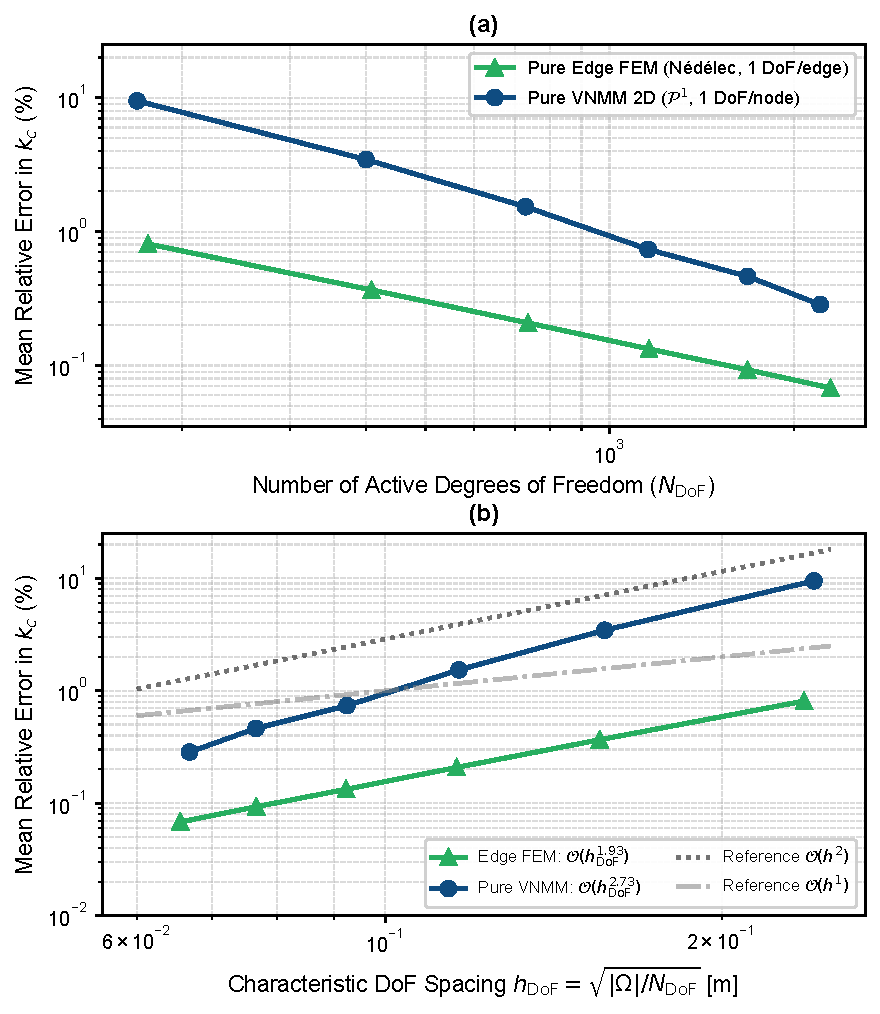
\includegraphics[width=0.62\linewidth]{figura_convergencia_vnmm_vs_fem.pdf}
    \caption{Spectral convergence comparison between Edge FEM and VNMM $\mathcal{P}^1$ for cavity $TE_z$ modes.
        (a) Mean relative error in cutoff wavenumber $k_c$ versus degrees of freedom $N_{\mathrm{DoF}}$;
        (b) Convergence versus characteristic spacing $h_{\mathrm{DoF}}$, showing fitted rates of $\mathcal{O}(h_{\mathrm{DoF}}^{1.93})$ (Edge FEM) and $\mathcal{O}(h_{\mathrm{DoF}}^{2.73})$ (VNMM).}
    \label{fig:convergence_vnmm_fem}
\end{figure}

\subsubsection{Convergence and Accuracy Comparison}
Table~\ref{tab:convergence_6_meshes} and Fig.~\ref{fig:convergence_vnmm_fem} report the convergence history across 6 successive mesh levels ($N \in \{9, 13, 17, 21, 25, 29\}$).

\begin{table}[!htbp]
    \centering
    \caption{Comparative convergence of resonant wavenumber $k_c$ for cavity $TE_z$ modes between Edge FEM and VNMM $\mathcal{P}^1$ across six refinement levels.}
    \label{tab:convergence_6_meshes}
    \resizebox{\columnwidth}{!}{%
        \begin{tabular}{@{} c *{3}{c} *{3}{c} @{}}
            \toprule
            \textbf{Mesh} & \multicolumn{3}{c}{\textbf{Edge FEM (N\'ed\'elec 1st-kind)}} & \multicolumn{3}{c}{\textbf{Pure VNMM 2D ($\mathcal{P}^1$ Complete Basis)}}                                                                         \\
            \cmidrule(lr){2-4} \cmidrule(lr){5-7}
            $N$           & $N_{\mathrm{DoF}}$                                           & $h_{\mathrm{DoF}}$ [m]                                                     & Error (\%) & $N_{\mathrm{DoF}}$ & $h_{\mathrm{DoF}}$ [m] & Error (\%) \\
            \midrule
            9             & 176                                                          & 0.2368                                                                     & 0.810      & 169                & 0.2417                 & 9.484      \\
            13            & 408                                                          & 0.1555                                                                     & 0.367      & 400                & 0.1571                 & 3.454      \\
            17            & 736                                                          & 0.1158                                                                     & 0.208      & 729                & 0.1164                 & 1.534      \\
            21            & 1160                                                         & 0.0922                                                                     & 0.133      & 1156               & 0.0924                 & 0.737      \\
            25            & 1680                                                         & 0.0766                                                                     & 0.093      & 1681               & 0.0766                 & 0.463      \\
            29            & 2296                                                         & 0.0656                                                                     & 0.068      & 2209               & 0.0668                 & 0.285      \\
            \bottomrule
        \end{tabular}%
    }
\end{table}

Inspection of the benchmark results reveals several noteworthy numerical properties:
\begin{itemize}
    \item \textbf{Strict Monotonicity and Quadrature Harmonization:} With the formulation of the scale-invariant dimensionless placement matrix $\widehat{\mathbf{A}}$ (Section~\ref{subsec:scale_invariant_criterion}), the support selection criterion $|\det(\widehat{\mathbf{A}})| \ge \widehat{\mathrm{Tol}}$ (operating at the stabilized value $\widehat{\mathrm{Tol}} = 0.80$) naturally preserves compact nearest-neighbor stencils ($K_{\mathrm{avg}} \approx 6.5$) on regular grids without requiring scale-dependent parameter tuning, preventing unphysical support dilation as $h \to 0$. Furthermore, employing node-conforming background cells ($N_{cx} = N_{cy} = N_v - 1$) with $3 \times 3$ Gauss points mitigates the artificial under-integration softening identified in the coarse $10 \times 10, 2 \times 2$ baseline of Section~\ref{subsubsec:quadrature_sensitivity}. Under the refined $3 \times 3$ quadrature employed here, the corresponding level $N = 21$ ($N_v = 36$, $1156$ DoFs, $35 \times 35$ cells) yields an error of $0.737\%$, and both Edge FEM and VNMM converge strictly monotonically toward the continuum limit as $h_{\mathrm{DoF}} \to 0$.
    \item \textbf{Theoretical Error Hierarchy and Absolute Precision:} Throughout all six refinement levels, Edge FEM delivers lower absolute errors ($0.810\%\text{--}0.068\%$ vs. $9.484\%\text{--}0.285\%$ for VNMM), reflecting the exact boundary circulation cancellation guaranteed by conforming edge spaces \cite{nedelec1980mixed, monk2003finite}.
    \item \textbf{Observed Convergence Slopes:} While Edge FEM consistently exhibits the canonical second-order rate across all levels ($\mathcal{O}(h_{\mathrm{DoF}}^{1.93})$, with local consecutive slopes tightly bounded between $1.88$ and $2.02$), the Pure VNMM solver displays an observed fitted slope of $\mathcal{O}(h_{\mathrm{DoF}}^{2.73})$ across the six tested refinement levels, steepening to $\mathcal{O}(h_{\mathrm{DoF}}^{2.97})$ on the four finest meshes (consecutive two-level slopes progressing from $2.34$ on $N=9 \to 13$, to $2.70$, $3.18$, $2.49$, and $3.54$).
    \item \textbf{Mesh-Free Discretization Advantage:} While Edge FEM maintains superior absolute accuracy for an identical DoF count on the evaluated regular geometry, the VNMM operates entirely without triangular mesh generation. This eliminates mesh quality degradation, element inversion, and remeshing bottlenecks in geometrically complex or topologically evolving electromagnetic domains.
\end{itemize}

\paragraph{Pre-Asymptotic Penalty Relief and Rayleigh Decomposition}
However, this steep fitted slope ($\mathcal{O}(h_{\mathrm{DoF}}^{2.73})$) must be interpreted with caution and should \emph{not} be construed as the theoretical asymptotic convergence order of the method. For conforming first-order affine polynomial representations $\mathcal{P}^1 \times \mathcal{P}^1$, standard conforming Galerkin variational theory bounds the asymptotic eigenvalue error by $\mathcal{O}(h^2)$ \cite{monk2003finite, boffi1999computational, boffi2013mixed}. In the present meshless setting, however, the global discrete space is non-conforming on unconstrained distributions ($V_h \not\subset H(\mathbf{curl};\Omega)$) due to dynamic stencil switching, meaning that conforming spectral estimates cannot be directly invoked as predictive guarantees.

This empirical rate acceleration is quantitatively explained by decomposing the discrete Rayleigh quotient into pure curl and penalty contributions: $\lambda = \lambda_{\mathrm{curl}} + s_{\mathrm{div}} \lambda_{\mathrm{div}}$, where $\lambda_{\mathrm{curl}} = \mathbf{e}^T \mathbf{K}_{\mathrm{curl}} \mathbf{e} / (\mathbf{e}^T \mathbf{M} \mathbf{e})$ and $\lambda_{\mathrm{penalty}} = s_{\mathrm{div}} \mathbf{e}^T \mathbf{K}_{\mathrm{div}} \mathbf{e} / (\mathbf{e}^T \mathbf{M} \mathbf{e})$. As reported in Table~\ref{tab:rayleigh_error_decomposition}, systematic tracking across all six refinement levels demonstrates that on the coarsest mesh ($N=9$, $169$ DoFs, $h_{\mathrm{DoF}} = 0.2417$\,m), the mean eigenvalue error ($20.16\%$) is strongly dominated by the penalty bias ($+24.94\%$), while the pure curl discretization error contributes only $-4.78\%$. Under progressive spatial refinement, discrete pointwise divergence rapidly vanishes ($\nabla \cdot \vec{E}^h \to 0$), causing the penalty bias to dissipate from $+24.94\%$ ($N=9$) down to $+5.79\%$ ($N=13$), $+2.44\%$ ($N=17$), $+1.41\%$ ($N=21$), and $+0.64\%$ ($N=29$), scaling with an empirical decay rate of $\approx \mathcal{O}(h_{\mathrm{DoF}}^{2.57})$. Concurrently, the pure curl discretization error converges monotonically toward the continuum limit ($-1.14\%$ at $N=29$). This measured partition confirms that the steep fitted slope ($\mathcal{O}(h_{\mathrm{DoF}}^{2.73})$) represents pre-asymptotic relief of coarse-grid penalty stiffening coupled with dynamic stencil consolidation, rather than an asymptotic super-convergence rate of the vector basis, while progressively narrowing, but not closing, the accuracy gap with Edge FEM (error ratio $\approx 11.7\times$ at $N=9$ and $\approx 4.2\times$ at $N=29$).

\begin{table}[!htbp]
    \centering
    \caption{Decomposition of discrete eigenvalue error into pure curl discretization error and divergence penalty bias across six refinement levels ($s_{\mathrm{div}} = 6.0$, $3 \times 3$ Gauss quadrature).}
    \label{tab:rayleigh_error_decomposition}
    \resizebox{\columnwidth}{!}{%
        \begin{tabular}{@{} c c c c c c c @{}}
            \toprule
            \textbf{Mesh} & $N_{\mathrm{DoF}}$ & $h_{\mathrm{DoF}}$ [m] & \textbf{Mean Error $k_c$ (\%)} & \textbf{Mean Error $\lambda$ (\%)} & \textbf{Curl Bias (\%)} & \textbf{Penalty Bias (\%)} \\
            \midrule
            9             & 169                & 0.2417                 & 9.484                          & 20.16                              & $-4.78$                 & $+24.94$                   \\
            13            & 400                & 0.1571                 & 3.454                          & 7.08                               & $+1.29$                 & $+5.79$                    \\
            17            & 729                & 0.1164                 & 1.534                          & 3.10                               & $+0.66$                 & $+2.44$                    \\
            21            & 1156               & 0.0924                 & 0.737                          & 1.48                               & $+0.03$                 & $+1.41$                    \\
            25            & 1681               & 0.0766                 & 0.463                          & 0.93                               & $-0.89$                 & $+1.42$                    \\
            29            & 2209               & 0.0668                 & 0.285                          & 0.57                               & $-1.14$                 & $+0.64$                    \\
            \bottomrule
        \end{tabular}%
    }
\end{table}

In summary, this benchmark demonstrates that the stabilized VNMM 2D achieves robust, monotonic spectral convergence that closely tracks canonical Edge FEM as the degree-of-freedom spacing decreases, while completely circumventing the topological meshing and geometric conformality requirements of edge-based simplicial methods. The unified scale-invariant threshold $|\det(\widehat{\mathbf{A}})| \ge \widehat{\mathrm{Tol}}$ and div-curl penalty ($s_{\mathrm{div}} = 6.0$) simultaneously guarantee compact support locality on regular lattices and prevent spurious gradient contamination within the evaluated operational bandwidth.

% ---------------------------------------------------------
% SUBSECTION 5.6: SPECTRAL VALIDATION ON IRREGULAR POINT CLOUDS WITH ARBITRARY DIRECTORS
% ---------------------------------------------------------
\subsection{Spectral Validation on Irregular Point Clouds with Arbitrary Vector Directors}
\label{subsec:spectral_irregular_clouds}

While Sections~\ref{subsec:cavity_eigenvalues} and \ref{subsec:convergence_comparison} validated spectral accuracy and benchmarked convergence against canonical Edge FEM using regular Cartesian grids with alternating directors (Eq.~\eqref{eq:alternating_directors_def}), assessing the practical utility of a meshless method demands solving the continuous vector boundary-value problem directly on \textbf{genuinely irregular point clouds with arbitrary unit vector directors}.

To appraise the numerical performance and robustness of the stabilized VNMM 2D ($\mathcal{P}^1$ complete basis, $s_{\mathrm{div}} = 6.0$) in the tested stochastic realization under simultaneous spatial and directional disorder, we discretize the square PEC resonant cavity $\Omega = [0, \pi]^2$ across six progressive refinement levels ($N \in \{9, 13, 17, 21, 25, 29\}$). To guarantee a strictly consistent comparison against the benchmark in Section~\ref{subsec:convergence_comparison}, the point clouds are constructed using the edge-equivalent nodal resolution parameter $N_v \in \{15, 22, 29, 36, 43, 49\}$ defined in Eq.~\eqref{eq:edge_equivalent_nv}, with nominal unperturbed generator grid spacing $h_{\mathrm{nom}} = L / (N_v - 1) = \pi / (N_v - 1) \in [0.2244, 0.0654]$\,m, active interior degrees of freedom $N_{\mathrm{DoF}} = (N_v - 2)^2 \in \{169, 400, 729, 1156, 1681, 2209\}$, and characteristic DoF spacings $h_{\mathrm{DoF}} = \sqrt{|\Omega|/N_{\mathrm{DoF}}} \in [0.2417, 0.0668]$\,m (Eq.~\eqref{eq:h_dof_definition}). The stochastic perturbation follows the protocol established in Section~\ref{subsec:stochastic_perturbations}:
\begin{enumerate}
    \item \textbf{Spatial Node Jitter ($25\%$):} Interior node coordinates are perturbed as $\mathbf{x}_k \leftarrow \mathbf{x}_k + [\delta x_k, \delta y_k]^T$, with independent random displacements $\delta x_k, \delta y_k \sim \mathcal{U}(-0.25\,h_{\mathrm{nom}}, 0.25\,h_{\mathrm{nom}})$, breaking Cartesian symmetry and producing a genuinely irregular spatial cloud.
    \item \textbf{Arbitrary Director Orientations:} Interior nodes are assigned unit vector directors with fully random azimuthal angles $\theta_k \sim \mathcal{U}(0, 2\pi)$, setting $\vec{t}_k = [\cos\theta_k, \sin\theta_k]^T$.
    \item \textbf{Boundary PEC Enforcement without Corner Nodes:} Boundary nodes are placed along the four cavity edges using the staggered face-centered configuration of Section~\ref{subsec:cavity_eigenvalues} (Eqs.~\eqref{eq:staggered_bnd_horiz}--\eqref{eq:staggered_bnd_vert}) at $(k + 0.5)\,h_{\mathrm{nom}}$, completely clearing the four domain corners/vertices by $h_{\mathrm{nom}}/2$. They strictly retain tangential alignment ($\vec{t}_k \parallel \partial\Omega$), enabling direct nodal collocation of homogeneous Dirichlet conditions ($\vec{E}^h(\mathbf{x}_k) \cdot \vec{t}_k = 0$) via $e_k = 0$.
\end{enumerate}

To ensure complete numerical parity with the structured benchmarks of Section~\ref{subsec:convergence_comparison}, numerical integration is executed under identical operational conditions: background cells aligned with the nodal spacing ($N_{cx} = N_{cy} = N_v - 1$), $3 \times 3$ Gauss-Legendre quadrature ($9$ points per cell), div-curl penalty $s_{\mathrm{div}} = 6.0$, and scale-invariant dimensionless thresholding $|\det(\widehat{\mathbf{A}})| \ge \widehat{\mathrm{Tol}}$ with $\widehat{\mathrm{Tol}} = 0.80$ and local normalization scale $h_{\mathrm{local}} = h_{\mathrm{nom}}$ (Section~\ref{sec:numerical_results}).

Table~\ref{tab:convergencia_cavidade_aleatoria} compiles the comparative convergence history across all six discretization levels between the structured Cartesian grid and the irregular point cloud, while Fig.~\ref{fig:convergencia_cavidade_aleatoria} illustrates the convergence trajectory and scaling behavior as functions of $N_{\mathrm{DoF}}$ and $h_{\mathrm{DoF}}$.

\begin{table}[!htbp]
    \centering
    \caption{Comparative spectral convergence of resonant wavenumber $k_c$ for cavity $TE_z$ modes on regular versus irregular point clouds across six refinement levels.}
    \label{tab:convergencia_cavidade_aleatoria}
    \resizebox{\columnwidth}{!}{%
        \begin{tabular}{@{} c *{3}{c} *{3}{c} @{}}
            \toprule
            \textbf{Mesh} & \multicolumn{3}{c}{\textbf{Regular Grid (Alternating Directors)}} & \multicolumn{3}{c}{\textbf{Irregular Cloud (25\% Jitter, Random $\theta_k$)}}                                                                         \\
            \cmidrule(lr){2-4} \cmidrule(lr){5-7}
            $N$           & $N_{\mathrm{DoF}}$                                                & $h_{\mathrm{DoF}}$ [m]                                                        & Error (\%) & $N_{\mathrm{DoF}}$ & $h_{\mathrm{DoF}}$ [m] & Error (\%) \\
            \midrule
            9             & 169                                                               & 0.2417                                                                        & 9.484      & 169                & 0.2417                 & 24.669     \\
            13            & 400                                                               & 0.1571                                                                        & 3.454      & 400                & 0.1571                 & 11.489     \\
            17            & 729                                                               & 0.1164                                                                        & 1.534      & 729                & 0.1164                 & 5.940      \\
            21            & 1156                                                              & 0.0924                                                                        & 0.737      & 1156               & 0.0924                 & 3.102      \\
            25            & 1681                                                              & 0.0766                                                                        & 0.463      & 1681               & 0.0766                 & 1.960      \\
            29            & 2209                                                              & 0.0668                                                                        & 0.285      & 2209               & 0.0668                 & 1.635      \\
            \bottomrule
        \end{tabular}%
    }
\end{table}

\begin{figure}[!htbp]
    \centering
    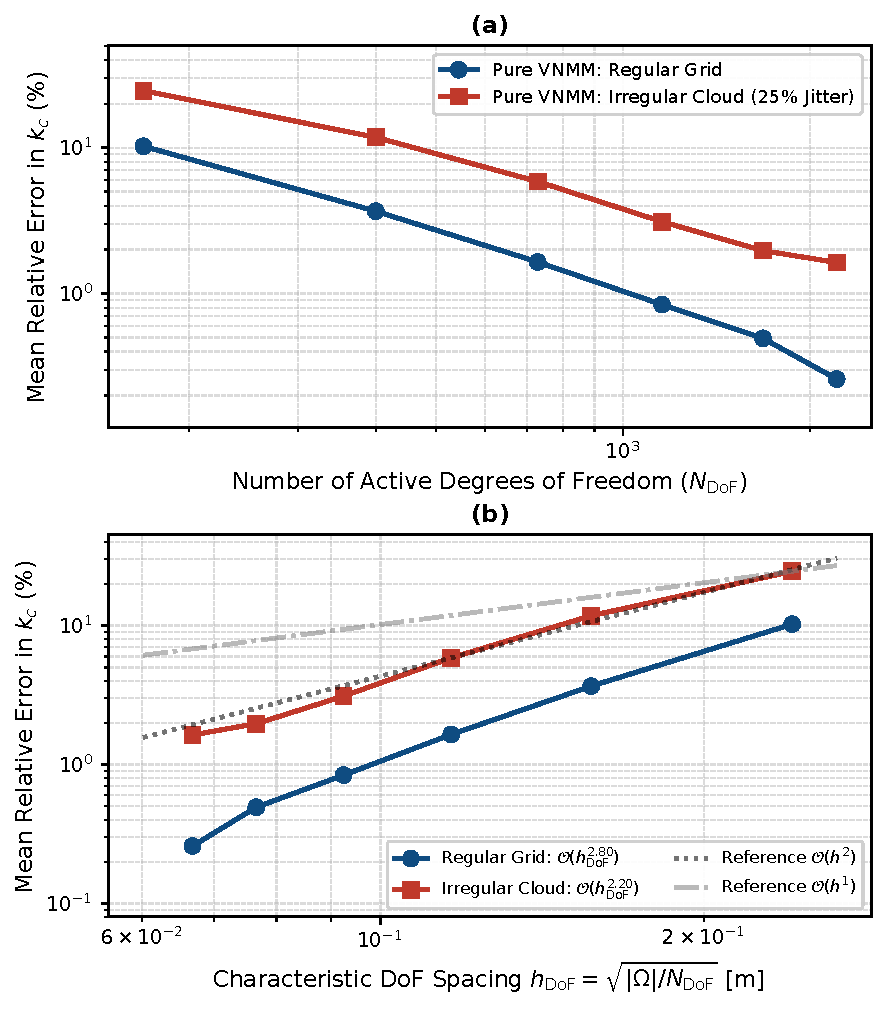
\includegraphics[width=0.62\linewidth]{figura_convergencia_cavidade_aleatoria.pdf}
    \caption{Spectral convergence of VNMM $\mathcal{P}^1$ on regular versus irregular point clouds.
        (a) Mean relative error in cutoff wavenumber $k_c$ versus degrees of freedom $N_{\mathrm{DoF}}$;
        (b) Convergence versus characteristic spacing $h_{\mathrm{DoF}}$, showing fitted slopes of $\mathcal{O}(h_{\mathrm{DoF}}^{2.73})$ (regular grid) and $\mathcal{O}(h_{\mathrm{DoF}}^{2.20})$ (irregular cloud).}
    \label{fig:convergencia_cavidade_aleatoria}
\end{figure}

Several critical findings emerge from the irregular point cloud eigenvalue benchmark:
\begin{enumerate}
    \item \textbf{Strict Monotonic Convergence under Spatial Disorder:} As evidenced in Table~\ref{tab:convergencia_cavidade_aleatoria} and Fig.~\ref{fig:convergencia_cavidade_aleatoria}a, the regularized VNMM converges strictly monotonically across all six refinement levels, with the mean cutoff wavenumber error decreasing from $24.67\%$ ($N = 9$, $h_{\mathrm{DoF}} = 0.2417$\,m) down to $1.64\%$ ($N = 29$, $h_{\mathrm{DoF}} = 0.0668$\,m). Across the tested resolutions, linear regression yields an observed fitted slope of $\mathcal{O}(h_{\mathrm{DoF}}^{2.20})$ as a function of the characteristic DoF spacing (Fig.~\ref{fig:convergencia_cavidade_aleatoria}b). As established in Section~\ref{subsec:convergence_comparison}, this empirical slope represents an observed rate in a non-conforming setting ($V_h \not\subset H(\mathbf{curl}; \Omega)$) rather than a universal theoretical guarantee. Significantly, the preservation of an empirical rate near $\mathcal{O}(h_{\mathrm{DoF}}^2)$ confirms that, for the evaluated stochastic sequence, the introduced spatial disorder and random director orientations do not trigger spectral stagnation or numerical locking, demonstrating monotonic convergence along the tested refinement path consistent with the complete linear polynomial space $\mathcal{P}^1$.

    \item \textbf{Error Hierarchy: Irregular vs. Regular Clouds:} Comparing the irregular cloud against the regular grid with alternating directors (Table~\ref{tab:convergencia_cavidade_aleatoria} and Fig.~\ref{fig:convergencia_cavidade_aleatoria}) reveals an expected error elevation on coarse discretizations ($24.67\%$ vs. $9.48\%$ at $N = 9$, and $3.10\%$ vs. $0.74\%$ at $N = 21$). This discrepancy stems from two coupled physical effects: (i) regular grids benefit from symmetry-induced partial cancellation of first-order Taylor truncation residuals, which is lost on irregular stencils; and (ii) coarse-cloud director misalignments generate localized non-zero divergence residuals ($\nabla \cdot \vec{E}^h \sim \mathcal{O}(h)$) that temporarily amplify penalty stiffening under $s_{\mathrm{div}} = 6.0$. As $h_{\mathrm{DoF}} \to 0$, this residual divergence vanishes, and the irregular cloud error converges monotonically toward the continuum limit, reaching $1.64\%$ at $N = 29$.

    \item \textbf{Spectral Purity and Absence of Spurious Modes in the Operational Band:} Table~\ref{tab:espectro_cavidade_aleatoria_fina} details the first 10 computed physical $TE_{nm}$ cavity modes for the fine irregular cloud ($N = 29$, $N_v = 49$, $N_{\mathrm{total}} = 2401$ nodes, $2209$ active DoFs). Despite the complete absence of grid symmetry and random director orientations, the div-curl formulation maintains clean spectral purity, shifting non-physical gradient nullspace branches outside the operational band ($\lambda \le 10$). All 10 lowest eigenvalues correspond strictly to physical cavity modes in exact 1-to-1 order with analytical references, yielding a global mean cutoff wavenumber error of $1.64\%$ (with individual mode errors ranging from $0.09\%$ for $TE_{02}$ to $2.71\%$ for $TE_{03}$).

    \item \textbf{Compact Support Locality and Search Efficiency:} Automated support selection preserves compact stencils across all irregular point clouds. Across the six evaluated refinement levels, the average number of candidate neighbors queried per Gauss point remains tightly bounded between $K_{\mathrm{avg}} = 6.34$ and $6.73$ (with the absolute maximum never exceeding $K_{\mathrm{max}} = 12$). This demonstrates that enforcing the scale-invariant threshold $|\det(\widehat{\mathbf{A}})| \ge 0.80$ enables the $k$-d tree early-stopping search to identify well-conditioned, regular sextets from immediate spatial neighbors, preventing support dilation and avoiding combinatorial overhead even under severe spatial-directional perturbations.
\end{enumerate}

\begin{table}[!htbp]
    \centering
    \caption{First 10 physical $TE_{nm}$ resonant cavity modes computed on the fine irregular point cloud against analytical references ($2{,}209$ active DoFs).}
    \label{tab:espectro_cavidade_aleatoria_fina}
    \resizebox{\columnwidth}{!}{%
        \begin{tabular}{@{} c c c c c c c @{}}
            \toprule
            \textbf{Mode ($TE_{nm}$)} & $\lambda_{\mathrm{analytical}}$ & $\lambda_{\mathrm{VNMM}}$ & \textbf{Error $\lambda$ (\%)} & $k_{c, \mathrm{analytical}}$ & $k_{c, \mathrm{VNMM}}$ & \textbf{Error $k_c$ (\%)} \\
            \midrule
            $TE_{10}$                 & 1.00                            & 0.9511                    & 4.89\%                        & 1.000                        & 0.975                  & \textbf{2.48\%}           \\
            $TE_{01}$                 & 1.00                            & 0.9544                    & 4.56\%                        & 1.000                        & 0.977                  & \textbf{2.31\%}           \\
            $TE_{11}$                 & 2.00                            & 1.9424                    & 2.88\%                        & 1.414                        & 1.394                  & \textbf{1.45\%}           \\
            $TE_{20}$                 & 4.00                            & 3.9493                    & 1.27\%                        & 2.000                        & 1.987                  & \textbf{0.64\%}           \\
            $TE_{02}$                 & 4.00                            & 3.9930                    & 0.17\%                        & 2.000                        & 1.998                  & \textbf{0.09\%}           \\
            $TE_{21}$                 & 5.00                            & 5.0366                    & 0.73\%                        & 2.236                        & 2.244                  & \textbf{0.37\%}           \\
            $TE_{12}$                 & 5.00                            & 5.1316                    & 2.63\%                        & 2.236                        & 2.265                  & \textbf{1.31\%}           \\
            $TE_{22}$                 & 8.00                            & 8.4144                    & 5.18\%                        & 2.828                        & 2.901                  & \textbf{2.56\%}           \\
            $TE_{30}$                 & 9.00                            & 8.5648                    & 4.84\%                        & 3.000                        & 2.927                  & \textbf{2.45\%}           \\
            $TE_{03}$                 & 9.00                            & 9.4952                    & 5.50\%                        & 3.000                        & 3.081                  & \textbf{2.71\%}           \\
            \midrule
            \textbf{Global Mean}      & ---                             & ---                       & \textbf{3.27\%}               & ---                          & ---                    & \textbf{1.64\%}           \\
            \bottomrule
        \end{tabular}%
    }
\end{table}

In summary, while these convergence results along the evaluated refinement sequence ($N = 9$ to $29$) confirm that the formulation maintains consistent $\mathcal{O}(h_{\mathrm{DoF}}^{2.20})$ accuracy without spectral corruption under the introduced spatial and directional disorder, they represent a specific stochastic realization. A formal discussion of the statistical scope and transferability of these irregular cloud benchmarks is presented next in Section~\ref{subsec:limitations_scope}.

% ---------------------------------------------------------
% SUBSECTION 5.7: LIMITATIONS AND SCOPE OF APPLICABILITY
% ---------------------------------------------------------
\subsection{Limitations and Scope of Applicability}
\label{subsec:limitations_scope}

While the numerical benchmarks in Sections~\ref{subsec:conforming_dual_equivalence}--\ref{subsec:spectral_irregular_clouds} confirm the accuracy, stability, and spectral purity of the proposed VNMM 2D formulation within the tested configurations, a rigorous computational framework requires delineating its operational boundaries and potential failure modes:

\begin{enumerate}
    \item \textbf{Background Quadrature Dependency:}
          Although local vector shape functions require no topological connectivity, evaluating the global Ritz-Galerkin weak form (Section~\ref{sec:variational_formulation}) currently relies on background integration cells with Gauss-Legendre quadrature. Because support stencils switch dynamically across and within integration cells, the resulting integrands exhibit piecewise non-polynomial jumps \cite{dolbow1999numerical}. As demonstrated in Section~\ref{subsubsec:quadrature_sensitivity} and Table~\ref{tab:quadrature_sensitivity}, capturing the true spatial discretization floor requires adequate cell refinement and integration density ($3 \times 3$ Gauss points), which reintroduces a geometric scaffolding burden in complex domains. Truly cell-free integration schemes (such as SCNI \cite{chen2001stabilized} or MLPG \cite{atluri2002meshless}) are discussed in Section~\ref{subsec:future_works}.

    \item \textbf{Global Non-Conformity and Trace Discontinuities:}
          Because support stencils are assembled independently across evaluation points, tangential traces between adjacent neighborhoods satisfy continuity only in a weak, approximate sense ($V_h \not\subset H(\mathbf{curl}; \Omega)$). Computationally, this lack of strong inter-element trace conformity produces non-vanishing curl residuals on discrete gradient fields ($\nabla_h \times \nabla_h \phi_h \neq \mathbf{0}$), requiring explicit volumetric div-curl penalty stabilization to prevent non-physical static states from contaminating discrete eigenvalue spectra.

    \item \textbf{Pathological Stencils, Boundary Starvation, and Geometric Curvature:}
          Automated support qualification assumes sufficient angular and spatial diversity in the candidate neighborhood. As cataloged in Section~\ref{subsec:singularities_P1} and Fig.~\ref{fig:vnmm_singularities_matrix_A}, local degeneracies arise primarily from near-parallel directors, near-collinear node distributions, or extreme aspect ratios ($\Delta x / \Delta y \gg 10$). In boundary layers or acute convex corners, geometric truncation restricts the accessible angular half-space, which can force the $k$-d tree search to query wider neighborhoods ($K > 12$), leading to localized support dilation and elevated conditioning. Furthermore, on non-orthogonal or curved boundaries, continuously rotating boundary tangents ($\vec{t}_k = \hat{\tau}(\mathbf{x}_k)$) introduce inter-element trace mismatch along adjacent boundary segments, yielding small residual tangential errors $[\hat{n} \times \vec{E}^h] \neq \mathbf{0}$ across background integration cells unless boundary stencils are geometrically enriched or aligned.

    \item \textbf{Transferability and Statistical Scope on Irregular Clouds:}
          While the scale-invariant criterion $|\det(\widehat{\mathbf{A}})| \ge \widehat{\mathrm{Tol}}$ successfully stabilizes the evaluated stochastically perturbed sequence under uniform nominal spacing (Section~\ref{subsec:stochastic_perturbations}), the observed convergence rate ($\mathcal{O}(h_{\mathrm{DoF}}^{2.20})$) and bounded conditioning are demonstrated for specific representative realizations. These findings should not be generalized as an absolute guarantee of robustness for arbitrary point clouds with multiscale clustering, acute boundary geometries, or alternative random seeds without systematic multi-seed statistical qualification.

    \item \textbf{Topological and Parametric Scope of Div-Curl Regularization:}
          While the div-curl regularizer effectively shifts non-solenoidal gradient modes outside the operational band, its applicability has clear theoretical boundaries (Section~\ref{subsubsec:div_curl_weak_form}):
          (i) it provides volumetric energy regularization rather than restoring point-to-point tangential trace conformity;
          (ii) it is restricted to simply connected, convex domains: in multiply connected geometries, harmonic 1-forms are divergence-free and require explicit topological cuts or circulation constraints \cite{bossavit1998computational, monk2003finite, gross2004electromagnetic}; and in non-convex domains with re-entrant corners, where singular fields lie outside $H^1$, penalty regularizations of this type are known to converge to a spectrum different from the Maxwell one unless weighted regularization is used \cite{costabel1991coercive, costabel2002weighted}; and
          (iii) the penalty parameter $s_{\mathrm{div}}$ is problem-specific, requiring calibration to ensure spectral clearance without inducing volumetric locking or ill-conditioning (Section~\ref{subsubsec:s_div_sensitivity}).

    \item \textbf{High-Frequency Electromagnetics and Phase Dispersion:}
          The present spectral validation focuses on the lower cavity resonant modes ($\lambda \le 20$). In high-frequency, short-wavelength regimes ($kh \gg 1$), numerical dispersion and phase lag (pollution effect) \cite{jin2014finite} require dense spatial sampling ($h \le \lambda_{\mathrm{EM}} / 10$). In electrically large domains, the penalty parameter $s_{\mathrm{div}}$ may require frequency-dependent scaling to preserve consistent spectral separation.

    \item \textbf{Dimensional Scope and Material Discontinuities:}
          The mathematical formulation is developed for two-dimensional electromagnetic fields ($xy$-plane, $TE_z$ polarization) in piecewise homogeneous PEC cavities. Extending the complete polynomial basis to 3D requires a 12-node stencil ($\mathcal{P}_1^3$), which significantly expands candidate search combinations (Section~\ref{subsec:future_works}). Furthermore, domains featuring sharp material interfaces ($\epsilon_{r1} \neq \epsilon_{r2}$) require subdomain-partitioned stencils to avoid unphysical smoothing across constitutive jumps.
\end{enumerate}

% =========================================================
% SECTION 6: CONCLUSION AND FUTURE WORKS
% =========================================================
\section{Conclusion and Future Works}
\label{sec:conclusion}

This work established a stabilized Vector Nodal Meshless Method (VNMM 2D) for electromagnetic vector field interpolation and eigenvalue analysis on unstructured point clouds without mesh connectivity. By resolving both the local polynomial incompleteness of early formulations and the global variational instabilities arising from mesh-free discretization, the proposed framework establishes the following core findings:

\subsection{Summary of Findings and Methodological Conclusions}
\label{subsec:summary_conclusions}

\begin{enumerate}
    \item \textbf{Resolution of Local Incompleteness ($\mathcal{L}^1 \to \mathcal{P}^1$):}
          Transitioning from the incomplete solenoidal basis $\mathcal{L}^1$ to the complete linear affine space $\mathcal{P}^1 = \mathcal{P}_1 \times \mathcal{P}_1$ resolves all independent entries of the first-order Jacobian $\nabla \vec{E}^h$. This overcomes the $\mathcal{O}(1)$ derivative noise floor observed on unconstrained clouds, restoring consistent $\mathcal{O}(h)$ curl convergence and accelerating electric field convergence to $\mathcal{O}(h^{2.17})$.

    \item \textbf{Scale-Invariant Support Selection ($\widehat{\mathbf{A}} + \text{$k$-d tree}$):}
          Formulating support qualification via the dimensionless placement matrix $\widehat{\mathbf{A}}$ removes the quartic scaling $\mathcal{O}(h^4)$, decoupling stencil geometry from absolute grid refinement. Enforcing $|\det(\widehat{\mathbf{A}})| \ge \widehat{\mathrm{Tol}}$ together with early-stopping $k$-d tree search preserves compact stencils ($K_{\mathrm{avg}} \approx 6\text{--}11$) down to the finest resolutions and empirically bounds local conditioning ($\kappa_2(\widehat{\mathbf{A}}) \le 5.9$) under $25\%$ spatial disorder.

    \item \textbf{Delineation of Topological Conformity vs. Mesh-Free Non-Conformity:}
          The formal proof of the Local Dual Equivalence Theorem establishes that VNMM reproduces lowest-order Whitney edge elements on conforming simplices down to machine precision ($\approx 10^{-16}$). On arbitrary clouds, however, moving support stencils destroy global trace continuity ($V_h \not\subset H(\mathbf{curl}; \Omega)$) and discrete de Rham sequence exactness, explaining why unregularized meshless vector eigenvalue problems inevitably suffer from gradient nullspace leakage.

    \item \textbf{Variational Div-Curl Regularization ($\mathbf{K}_{\mathrm{curl}} + s_{\mathrm{div}} \mathbf{K}_{\mathrm{div}}$):}
          Volumetric div-curl regularization provides effective spectral stabilization without expanding system dimensions. Within the calibrated operating window ($s_{\mathrm{div}} \in [6.0, 10.0]$), spurious gradient modes are shifted past the operational spectrum ($\lambda_{\mathrm{spur}} = 10.16 > 9.39$) while solenoidal physical resonances remain practically unperturbed ($R_{\mathrm{div}} \le 0.87\%$). Systematic multi-level tests show empirical refinement slopes of $\mathcal{O}(h_{\mathrm{DoF}}^{2.73})$ on regular lattices and $\mathcal{O}(h_{\mathrm{DoF}}^{2.20})$ across the evaluated stochastic sequence down to $1.64\%$ cutoff error.

    \item \textbf{Operational Scope and Canonical Validation Boundaries:}
          The present results validate the foundational mathematical framework, algebraic singularity elimination, and spectral stabilization on 2D canonical PEC cavities under $TE_z$ polarization. These benchmark findings demonstrate consistent empirical convergence and bounded conditioning along the tested regular and stochastically perturbed sequences, but should not be extrapolated as universal guarantees for arbitrary point distributions or complex engineering problems. Extending the method to real-world electromagnetic devices requires addressing the open practical challenges identified in Section~\ref{subsec:limitations_scope}: non-orthogonal curved boundaries, multi-seed statistical qualification, subdomain-partitioned stencils for sharp dielectric interfaces, and frequency-adaptive stabilization.
\end{enumerate}

\subsection{Promising Directions for Future Research}
\label{subsec:future_works}

Building upon this 2D stabilized vector formulation, several key avenues remain for future investigation:
\begin{enumerate}
    \item \textbf{Extension to 3D Vector Formulations:}
          Extending the complete polynomial vector basis to three dimensions ($\mathcal{P}_1 \times \mathcal{P}_1 \times \mathcal{P}_1$, requiring $M_{\mathrm{supp}} = 12$ nodes per stencil) to model 3D resonant cavities, waveguiding structures, and radiation problems \cite{goncalves2023vector}.

    \item \textbf{Cell-Free Quadrature and Complex Boundaries:}
          Replacing background integration cells with cell-free schemes---such as Stabilized Conforming Nodal Integration (SCNI) \cite{chen2001stabilized} or MLPG subdomains \cite{atluri2002meshless}---to eliminate background quadrature scaffolding and better accommodate moving, multi-scale, or curved domain boundaries.

    \item \textbf{Multi-Seed Statistical Characterization:}
          Conducting extensive Monte Carlo campaigns across multiple independent random cloud realizations per refinement level to compute statistical error distributions (mean and standard deviation), worst-case condition numbers, and stencil qualification failure rates across diverse cloud generation algorithms and boundary geometries.

    \item \textbf{Subdomain-Partitioned Stencils for Material Interfaces:}
          Developing multi-tree spatial data structures \cite{parreira2006efficient} to restrict candidate stencils to homogeneous subdomains, preserving sharp constitutive parameter jumps ($\epsilon_{r1} \neq \epsilon_{r2}$) and weakly enforcing normal flux continuity across material discontinuities.

    \item \textbf{Weak Trace Enforcement and Discontinuous Galerkin Frameworks:}
          Investigating interior penalty Discontinuous Galerkin (IP-DG) \cite{hesthaven2004high, houston2004mixed} or hybridized discontinuous Galerkin (HDG) trace formulations \cite{nguyen2011hybridizable} evaluated across background cell interfaces to penalize tangential trace jumps $[\hat{n} \times \vec{E}^h]$ between adjacent support domains, weakly restoring discrete de Rham exactness as an alternative to volumetric div-curl penalty regularization.

    \item \textbf{Hybrid EFEM--VNMM Coupling:}
          Developing hybrid domain-decomposition formulations that couple canonical Edge Finite Elements (EFEM) with the stabilized VNMM. In this multi-paradigm framework, EFEM is deployed in bulk regions where conformal simplicial or hexahedral meshes are straightforwardly generated, while VNMM discretizes regions characterized by geometric complexity, severe spatial variations, or narrow gaps where meshing is burdensome. Interface coupling between edge circulations and meshless directional degrees of freedom can be directly established through the constructive Whitney equivalence proved in Section~\ref{subsec:conforming_dual_equivalence}, providing seamless transition and exact tangential compatibility without auxiliary interface variables.

    \item \textbf{Non-Linear Media and Electrical Machine Motion Modeling:}
          Building directly upon the hybrid EFEM--VNMM framework, coupling the formulation with non-linear Newton-Raphson iterations and time-stepping algorithms to model electromagnetic devices with moving parts. In rotating electrical machines, for instance, EFEM can model stationary slotted stator and rotor magnetic cores under ferromagnetic saturation ($B\text{--}H$ curves), while VNMM discretizes the intervening air gap, naturally accommodating continuous rotor motion and geometric eccentricity without remeshing, sliding-surface interpolation artifacts, or mesh distortion \cite{coppoli2012induction}.
\end{enumerate}


\section*{Declaration of Generative AI and AI-Assisted Technologies in the Writing Process}
During the preparation of this work, the authors used Google Antigravity / Gemini in order to assist with English language editing, LaTeX code formatting, script automation for numerical data consistency, and cross-referencing verification. After using this tool, the authors carefully reviewed, verified, and edited all resulting content and take full responsibility for the integrity and accuracy of the publication.

\section*{CRediT Authorship Contribution Statement}
\textbf{Renato C. Mesquita}: Conceptualization, Methodology, Software, Formal analysis, Investigation, Writing -- original draft, Writing -- review \& editing, Visualization, Supervision, Funding acquisition.
\textbf{Elson J. da Silva}: Conceptualization, Formal analysis, Writing -- review \& editing.
\textbf{Bárbara M. F. Gonçalves}: Methodology, Software, Validation, Investigation, Formal analysis, Writing -- review \& editing.
\textbf{Luilly A. G. Ortiz}: Methodology, Software, Validation, Data curation, Writing -- review \& editing.

\section*{Declaration of Competing Interest}
The authors declare that they have no known competing financial interests or personal relationships that could have appeared to influence the work reported in this paper.

\section*{Data and Code Availability}
The source code, simulation scripts, benchmark datasets, and point-cloud generation algorithms supporting the findings of this study are publicly available on GitHub at \url{https://github.com/rencmbr/vnmm2d-eabe}.

% --- AGRADECIMENTOS ---
\section*{Acknowledgements}
The authors would like to thank the Brazilian research funding agencies CAPES, CNPq, and FAPEMIG for their financial support during the development of this research project. In particular, R.~C.~Mesquita acknowledges financial support from CNPq through the Senior Research Productivity Fellowship (Process: 305185/2026-8).

% --- REFERÊNCIAS BIBLIOGRÁFICAS ---
\bibliographystyle{elsarticle-num}
\bibliography{references-longversion}

\end{document}

\endinput
%%
%% End of file `elsarticle-template-num.tex'.